% AER-Article.tex for AEA last revised 22 June 2011
\documentclass[reviewmode,AEJ]{AEA}

% The mathtime package uses a Times font instead of Computer Modern.
% Uncomment the line below if you wish to use the mathtime package:
\usepackage{mathptmx}

% Note that miktex, by default, configures the mathtime package to use commercial fonts
% which you may not have. If you would like to use mathtime but you are seeing error
% messages about missing fonts (mtex.pfb, mtsy.pfb, or rmtmi.pfb) then please see
% the technical support document at http://www.aeaweb.org/templates/technical_support.pdf
% for instructions on fixing this problem.

% Note: you may use either harvard or natbib (but not both) to provide a wider
% variety of citation commands than latex supports natively. See below.

% Uncomment the next line to use the natbib package with bibtex 
\usepackage{natbib}

% Uncomment the next line to use the harvard package with bibtex
%\usepackage[abbr]{harvard}

\usepackage[hidelinks]{hyperref}
\usepackage{booktabs}
\usepackage{enumitem}
\usepackage{tabularx}
\usepackage[input-symbols = ()]{siunitx}
\usepackage{lscape}
\usepackage{graphicx}
\usepackage{placeins}
\usepackage{setspace}
\usepackage{amsmath}
\usepackage{float}

\usepackage[title]{appendix}

% \usepackage{fullpage}

\renewcommand{\floatpagefraction}{1}
\renewcommand*{\bibfont}{\footnotesize}

\raggedbottom

% This command determines the leading (vertical space between lines) in draft mode
% with 1.5 corresponding to "double" spacing.
% \draftSpacing{1.5}

% break up long URL at hyphens
\def\UrlBreaks{\do\/\do-}

\sisetup{
	detect-all,
	round-integer-to-decimal = true,
	group-digits             = true,
	group-minimum-digits     = 3,
	round-mode				 = off, 
	round-precision			 = 3,
	group-separator          =  {,},
	table-align-text-pre     = false,
	table-align-text-post    = false,
	group-digits			 = integer,
	input-signs              = + -,
	input-symbols            = {*} {**} {***},
	input-open-uncertainty   = ,
	input-close-uncertainty  = ,
	retain-explicit-plus
}

\newtheorem{proposition}{Proposition}

\begin{document}
% \onehalfspacing

\title{Making Lemonade from Lemons: Taxi Drivers' Response to Cancellations and No-shows}
\shortTitle{Making lemonade from lemons}
\author{Hai Long Duong, Junhong Chu and Dai Yao\thanks{Duong: NUS Business School, Business Link 1, Singapore, bizdhl@nus.edu.sg. Chu: NUS Business School, 15 Kent Ridge Drive, Singapore, bizcj@nus.edu.sg. Yao: NUS Business School, 15 Kent Ridge Drive, Singapore, dai.yao@nus.edu.sg. We gratefully acknowledge funding from Singapore Ministry of Education Social Science Research Thematic Grant, MOE2016-SSRTG-059, SPIRE. We are very grateful to one of the leading taxi companies in Singapore for providing us with the data for this research, and deeply indebted to its management team for sharing with us their insights on the taxi industry.}}
%\date{\today}
%\author{}
%\pubMonth{}
%\pubYear{}
%\pubVolume{}
%\pubIssue{}
\JEL{J22, J24, D91}
%\Keywords{labor supply, productivity, cancellation, no-show, taxi driver, sharing economy, big data}


\begin{abstract}
	%We study the impact of booking cancellations and passenger no-shows on taxi drivers' labor supply and productivity. We employ a novel large dataset that covers three months of taxi bookings and street hail trips for one major taxi operator in Singapore. We find that drivers work longer and earn more per hour following cancellations or no-shows, as if they strive to make up for the loss from such adverse actions. Working longer and increasing productivity are substitutable rather than complementary devices, and are chosen by taxi drivers in their own favor: More experienced drivers tend to increase productivity, and solo drivers tend to work more hours. 
	\citet{kHoszegi2006model} show that workers with endogenous income targets respond differently
	to anticipated changes and unanticipated shocks in their earnings, and only the latter generates
	behaviors that contradict the neoclassical model of labor supply. In this paper, we study the
	impact of booking cancellations and passenger no-shows---a source of unanticipated negative 
	income shocks---on Singaporean taxi drivers' labor supply and productivity. We find that 
	drivers work longer and earn more per hour following cancellations or no-shows. This provides 
	compelling evidence for income targeting labor supply, even in the presence of endogenous 
	reference point. In addition, we find that drivers respond more strongly to more recent 
	cancellations and no-shows, suggesting a dynamic nature of the reference point. Moreover, 
	working longer and increasing productivity are substitutable rather than complementary devices, 
	and are chosen by taxi drivers in their own favor: More experienced drivers tend to increase 
	productivity, and solo drivers tend to work more hours. 
\end{abstract}

\maketitle



\section{Introduction}
\label{sec:intro}

Despite being a building block for many economic models and playing an imperative role in the 
design of numerous public policies and industrial practices, labor supply is still a controversial 
topic in economics. The two competing theories are the neoclassical labor supply model, which 
predicts temporal substitution of leisure for labor when wage rises, and the income target model, 
which predicts that workers have a target level of income, which, together with loss aversion, 
motivates them to work harder when wage is low. Empirical studies have shown mixed results not 
only in different settings, but sometimes even in the same setting using different methodologies.
A prominent example is the taxi industry, in which seminal work by \citet{camerer1997labor} and 
later papers, such as \citet{crawford2011new}, \citet{martin2017quit}, and \citet{thakral2018daily}, 
find evidence for drivers' daily income target. Other studies, such as 
\citet{farber2005tomorrow,farber2015you}, find stronger support for the neoclassical model.

To reconcile these mixed results, \citet{kHoszegi2006model} propose a model of reference-dependent 
preference that formalizes the notion of income targeting while allowing for neoclassical behaviors 
to exist under certain circumstances. The model's key insight is that sophisticated workers can 
form their target rationally; for them, reference dependence only matters if the variation in wages 
is \textit{unanticipated}, because they will adjust their target in response to anticipated 
changes in a manner that is consistent with the neoclassical model.

Empirical studies of daily labor supply have largely overlooked this distinction between 
anticipated changes and unanticipated shocks\footnote{ Only a few papers explicitly consider this 
distinction: \citet{agarwal2017anticipated} investigate the effects of a large anticipated one-time 
income shock due to a pension withdrawal at age 55, while \citet{andersen2014toward} conduct field 
experiments  introducing expected and unexpected earnings shocks to vendors in an Indian 
open air market.}. A common test of reference-dependent labor supply is to show a relationship 
between intra-day income---either in the form of cumulative earnings up to a point in time, or 
total earnings during a specific time interval of the day---and subsequent labor supply decisions. 
However, an insignificant result of this test does not entirely reject reference dependence; it may 
simply reflect the low level of unanticipated shocks experienced by workers within that specific time 
and context, or an anticipation formation process that is extremely adaptive to new shocks. 
For instance, \citet{farber2015you} finds a marginal effect of income on stopping decisions in day 
shifts, but positive wage elasticity due to negligible variation in transitory unanticipated hourly 
wage changes among New Year City (NYC) taxi drivers. \citet{thakral2018daily} point out that if the 
reference point adjusts to recent earnings at a sufficiently fast speed, a reference-dependent worker 
may act in a manner similar to a neoclassical worker. Several papers use structural models to 
explicitly account for a worker's anticipation, but this approach requires strong assumptions about 
how the reference point is formed---and since the reference point is unobserved, these assumptions 
are difficult to test. As a result, using variation in realized daily earnings constitutes, at best, 
only a weak test for reference dependence, and at worst, can be misleading about the nature of the 
labor supply response.

We propose the use of an alternative approach, by exploiting \textit{unanticipated} sources of external 
income shocks that workers encounter repeatedly over time and examining how these shocks affect workers' 
subsequent labor decisions. We focus on Singapore's taxi industry, and the income shocks we use are 
booking cancellations and passenger no-shows---i.e., in which a passenger makes a booking but fails 
to follow through with the trip, resulting in the loss of time, mileage, and potential earning 
opportunities for the driver. Passengers' decisions to cancel a booking or not show up are made with 
little interaction with the driver, and hence are unlikely to be predicted by drivers and factored 
into their daily income target prior to the booking. Since the subsequent wage rate is not affected 
by these idiosyncratic events, the neoclassical model would predict no relationship between cancellations 
and no-shows (C\&NS hereafter) and the subsequent supply of labor. In contrast, under reference-dependent 
preference, we would expect drivers to work harder because after C\&NS, their realized earnings will fall 
below the typical level they can achieve with the same amount of worked hours but without C\&NS. 
Essentially, we single out a source of income shocks that is reliably unanticipated, which enables 
us to construct a transparent test for reference-dependent preference and a straightforward 
interpretation of the results.


This paper also addresses a growing question in the reference dependence literature: How is the 
reference point determined? If the reference point is fixed, wage elasticity of the labor supply will be
close to $-1$ and there will be little variation in daily income---an outcome that is easily rejected 
in most contexts that involve flexible-hour workers. To explain the high variation in daily income among 
these workers, some form of the reference point's ability to adapt to market conditions must be present. 
In the context of the NYC taxi industry, \citet{thakral2018daily} show that the reference point can even 
respond to within-day earning variation, and more recent earnings have a greater effect on labor supply 
than earlier earnings. Our approach of using unanticipated income shocks complements this line of research. 
C\&NS, our source of income variation, are random events that can occur anytime during the day, and their
timing can be used to test the dynamic nature of the reference point. A recent C\&NS and a C\&NS that 
occurred early in the shift, given similar characteristics, cost drivers the same amount of potential 
earnings---and hence, under a static reference point, would have the same effect on subsequent labor 
decisions. On the other hand, if drivers continually adjust the reference point when new shocks come in, 
we would expect the effects of recent and earlier C\&NS to be different. This constitutes a complementary, 
albeit more direct and transparent, alternative to  \citeauthor{thakral2018daily}'s test of adaptive 
reference dependence.

\paragraph{Settings} The taxi industry has been of great interest to economists due to its special work 
arrangement, which enables empirical tests of various competing economic theories. In particular, 
Singapore's taxi market has attracted considerable attention from researchers \citep{Ho3074,chou2002testing,agarwal2015singaporean,agarwal2017anticipated,agarwal2018fickle}, 
thanks to not only data availability but also several unique features of the market. The typical 
arrangement in Singapore is for the taxi operator to lease cabs to drivers using specific rate schemes,
and drivers freely choose how long to work each day.
%Put another way, the taxi operator has “sold the firm” to drivers, and each driver plays the 
%role of a self-employed entrepreneur, internalizing in his own venture all of the costs and benefits 
%of supplying labor. 
One feature of Singapore's taxi industry that differentiates it from the extensively studied NYC yellow 
cab market is that it is common for customers to book taxi services via telephone, SMS, the internet, 
and mobile apps, whereas in NYC cabs are mostly hailed on the street\footnote{A number of for-hire vehicle
companies in NYC provide prearranged transport service, but the number of trips completed by these companies 
is relatively small compared to yellow cab trips (Taxi and Limousine Commission Factbook, 2016). Recently,
several mobile apps such as Curb have been developed to allow yellow and green cabs in the city to accept
bookings (see https://www.theverge.com/2016/3/23/11294758/curb-app-taxi-hail-uber-nyc-verifone).}. 
With the arrival of ride-hailing services such as Uber and Grab, customers in Singapore are becoming more
accustomed to booking their rides, and taxi operators are increasingly promoting their own booking systems
to remain competitive\footnote{See \citet{agarwal2018fickle} for a study on the interaction between taxi 
bookings and ride-hailing platforms in Singapore.}. In essence, Singapore's taxi industry is a combination 
of traditional taxi services and a modern ride-hailing platform.

%There are two main reasons for our focus on booking cancellations and passenger no-shows as the negative shock of interest in this market. First, conditional on market conditions and drivers' bidding for bookings, C\&NS are \textit{exogenous} events from the drivers' perspective, as these actions are entirely customers' decisions. Moreover, the booking system provides nothing but the estimated time of arrival and the vehicle's plate number to the customer, and hence it is unlikely that customers' actions are influenced by driver characteristics such as gender, race, or age, as is common in other markets \citep{mejia2018transparency,cui2016discrimination,edelman2017racial,NBERw22776}. This enables clean identification of the effects of C\&NS on driver behavior. In our analyses, we use a rich set of control variables and fixed effects to absorb the impacts of aggregate demand and supply conditions, as well as drivers' propensity to bid for a booking, and hence the estimated effects of C\&NS reflect drivers' responses to customers' adverse actions.

%Second, C\&NS are a relatively common phenomenon in many, if not all, services. While a large literature is devoted to them, most studies \citep{moore2001time,liu2010dynamic,feldman2014appointment,zacharias2014appointment} have focused only on operational aspects and have largely ignored the behavioral effects of these actions, such as how they impact workers' morale and motivation. From an operational perspective, it is straightforward to see that C\&NS generate lost sales, and the associated uncertainty entails the use of additional resources such as buffer time, stand-by personnel, rescheduling capacity, etc., which can be costly to service providers. In this paper, we show that C\&NS can also induce behavioral changes from agents on the supply side, and these changes may not always go in the same direction as operational effects.

%This paper focuses on two dimensions of labor behavior: labor supply and productivity. First, we ask how C\&NS affect drivers' propensity to end their shifts. Second, we ask how the rate of earnings change after experiencing a C\&NS. Third, we investigate the dynamics of these effects, i.e., how drivers' responses change over time. Specifically, we examine how a C\&NS in the current hour affects driver behavior, not only in the current hour but also in each of the subsequent hours. Fourth, we examine the interrelationship between the two behavioral adjustments, labor supply versus productivity, by examining heterogeneous effects among groups of drivers who have a comparative advantage in one type of adjustment. Specifically, we look at how solo drivers, who do not share their taxi with another driver and therefore have an advantage in terms of prolonging their working hours, adjust their labor supply and how more experienced drivers, who have an advantage in terms of skill---and hence tend to be better at managing their productivity---adjust their productivity. Analysis of these dynamics and heterogeneous effects will yield suggestive evidence about the underlying mechanisms that drive these behavioral responses.

\paragraph{Data and Methodology} We exploit a novel dataset provided by a major taxi operator in Singapore,
which covers 3 months of street hail trips and taxi bookings by more than 30,000 drivers and comprises 34
million observations for the period December 1, 2016--February 28, 2017. To the best of our knowledge, 
this is the first taxi dataset of this size used in a research study that contains detailed information 
about not only street hail trips and taxi bookings, but also C\&NS. 

We employ fixed-effect regression as our main methodology, utilizing multiple sets of fixed effects 
to absorb unobserved market conditions and driver characteristics. We also leverage the rich set of 
features present in our dataset to address various endogeneity concerns. Our estimates are robust, 
in terms of both direction and magnitude, across a wide range of specifications. We conduct a placebo 
test to further confirm that our results are not driven by unobserved market factors or selection. Lastly, 
although our main specification is linear, we have conducted extensive specification checks that allow for
various forms of non-linearity to confirm that our results are not driven by functional assumptions.

As a robustness check, we also employ instrumental variable approach, using the free taxicab count nearby 
the pickup location and around the booking time as exogenous source of variation to vary C\&NS rate.
The rationale and the results of this approach are discussed in Appendix \ref{apx:iv}. 
Since the exogeneity test fails to reject the exogeneity of C\&NS, 
we choose to use fixed-effect linear regression as our main approach.


\paragraph{Main results} Our analysis shows that drivers work longer and earn more per hour following 
C\&NS, apparently seeking to compensate for the loss and to reach the income target. Longer work hours 
and increased productivity can reverse the negative impact of cancellations, leading to higher income 
for the shift. However, they can only fully offset the negative impact of no-shows on shift income, 
due to more time wasted by no-shows. Interestingly, working longer and increasing productivity are 
substitutable rather than complementary devices, and are chosen by taxi drivers in their own favor: 
More experienced drivers, with better job search skills than less experienced ones, tend to work more 
diligently to increase their productivity; solo drivers, with a more flexible schedule than sharing 
drivers, tend to work more hours. Furthermore, these effects are strong in the first hour after a 
C\&NS and fade away afterward. Interestingly, the C\&NS effects are strongest when cumulative income 
is moderate and close to the average shift income, and become weaker and insignificant when the income 
level is too high or too low. 

\paragraph{Interpretation} Our results, collectively, suggest income targeting behavior to be the explanation
for the C\&NS effects on labor supply. The alternative explanation that C\&NS effects are driven by lower
fatigue or lower disutility of work after a C\&NS is unlikely because cumulative income level has a significant 
moderating effect on the C\&NS effects. There is no reason for the effect of fatigue to be different at 
different cumulative income levels. On the contrary, the income target theory provides a consistent explanation
for such phenomenon: If the driver is too far below the target, a small earnings shock from a C\&NS may not
meaningfully change the chance of achieving the target as much as when the driver is very close to the target; 
if the driver is too far above the target, a C\&NS will not move him from the gain domain to the loss domain
and thus he has no incentive to change his behavior. Moreover, according to our conversations with drivers 
and the feedback from the taxi operator, C\&NS are commonly viewed as a nuisance rather than an opportunity
for a breather. Vehicle utilization and earnings rate increase after C\&NS, and hence it is unlikely that
the drivers catch a short break following C\&NS. We also rule out the possibility of immediate pickups or
other events immediately following C\&NS, rather than the C\&NS themselves, causing the change in labor 
supply. The most plausible interpretation of the C\&NS effects is income targeting: C\&NS lower the 
driver's total earnings given the same duration of work, which motivates him to work longer and harder
to reach the daily target. 

\paragraph{Economic significance} The magnitude of the C\&NS effects is economically significant: A C\&NS
is associated with 31\% to 33\% reduction from the mean hazard rate of stopping work at a given time. 
This is equivalent to the effects of additional 55 minutes of work, or additional 48 Singapore dollars 
(SGD, 1 SGD = 0.7 USD during the data period) of realized earnings having on the decision to stop 
(Table \ref{tb:robustquit}, Column (7)). From our personal interactions with drivers and the taxi 
operator,  C\&NS are frequent enough, with an average occurrence rate of between once or twice every
week, to be a significant concern in their work. More importantly, our paper uses C\&NS as an example
for unanticipated earnings shocks, and C\&NS are far from being the only unanticipated nuisance that 
taxi drivers encounter daily. Even though \cite{farber2015you} claims that  unanticipated earnings only
account for a small proportion of the total variation in NYC taxi drivers' daily income, subsequent 
studies sometimes reach contrary findings. Both \cite{thakral2018daily} and \cite{martin2017quit} 
find evidences in support of income targeting---also among NYC taxi drivers---by employing more flexible
specification. The relevance of unanticipated earnings may depend on context, and drivers at certain time 
and in certain places may experience more of such shocks than others. There are several reasons why 
Singapore's taxi drivers may find unanticipated earnings more prominent: the complex topography of 
the city, the existence of a booking system, the competition from a public transport network that 
regularly expands, etc. Moreover, the proportion of taxi bookings is increasing rapidly over years, 
making C\&NS more important to the drivers day by day. 

\paragraph{Contributions} Our paper makes three contributions to the literature on daily labor supply 
of flexible-hour workers. The first is to provide a new, cleaner testing approach and new, more compelling
evidence for reference-dependent labor supply. Our results provide strong evidence for reference-dependent 
preference among Singapore's taxi drivers, which is not a surprise given the mixed findings from numerous 
studies in similar contexts. The novel aspect of our results is that we obtain such findings by exploiting
an \textit{unanticipated} source of random income shocks, C\&NS, that are naturally encountered by workers
in the market to identify the income reference effect. This constitutes a direct and stronger test for the
class of reference-dependent preference models described by \citet{kHoszegi2006model} or any models that 
allow the reference point to adjust to workers' anticipation. This extends the literature, because the
interpretation of our results is free of concern about the relative strength of anticipated versus 
unanticipated variation in income or the exact process by which the reference point is formed.

In addition, our independent variables, C\&NS, are not only unanticipated, but also \textit{externally} 
determined---since they are passengers', not drivers', decisions---which enables a better identification
strategy. Previous studies use two common approaches to identify reference dependence. The first is to
look for negative correlation between hours of work and average daily wage, as in \citet{camerer1997labor}. \citet{oettinger1999empirical} and \citet{farber2005tomorrow}  criticize this approach on three grounds:
(1) the use of realized earnings, which are an equilibrium outcome, as a proxy for wage rate is questionable; 
(2) wages are not constant within a day, and using average daily wage may constitute a misspecification; and
(3) construction of the wage rate, by dividing total earnings by total hours of work, is prone to measurement
error and division bias. The second approach is to examine the correlation between intra-day earnings and
the hazard of stopping work throughout the day. Although this approach reduces concern about measurement 
error and division bias, and is able to account for the dynamic nature of earnings and labor supply, it is
not entirely free of potential endogeneity issues. Intra-day income, in the form of either cumulative earnings 
up to a certain point in time, or total earnings in a specific hour into the shift, is an outcome variable 
jointly determined by market demand and workers' behaviors, and is likely correlated with unobserved market 
factors and workers' characteristics that may also contribute to workers' decision to stop working. 

In contrast, the shocks we use in this paper---decisions made by agents on the other side of the market without
any direct interaction with workers---are external, and hence unlikely to be subject to confounding factors 
due to unobserved worker heterogeneity. The shocks may still be correlated with market conditions, however, 
and to address this issue we leverage our novel dataset to construct a rich set of control variables---arguably 
the most detailed set of controls in this line of study so far. Even in this regard, our approach still tends
to be more reliable because the set of confounding market factors that pose a threat to our identification 
strategy must be those that influence two different kinds of decisions by two different agents: passengers'
decisions to cancel or not show up and workers' decisions to continue supplying labor. This set is likely
to be much smaller than the set of market factors that influence two related outcomes by the same agent,
workers' earnings and labor supply, that may bias estimates using the intra-day income approach.


Our second contribution is that our results provide clean and convincing evidence for the adaptive nature
of the reference point. This complements findings in the growing literature on the path of reference points
over time \citep{dellavigna2017reference,thakral2018daily}. We find that the timing of income shocks matters:
A recent C\&NS has a stronger effect on labor decisions, and the effect lasts for no more than 2 hours. 
In this regard, our results are most closely related to those of \citet{thakral2018daily}, who find that 
recent earnings have stronger effects on the hazard of stopping work than distant earnings in the same day.
In one of our specifications, we account for \citeauthor{thakral2018daily}'s effects by controlling for
individual earnings during a different time period in the shift, but C\&NS effects persist. Therefore,
though similar in nature, \citeauthor{thakral2018daily}'s model does not entirely explain our results. 
It also shows that different sources of income shocks may change the reference in different ways, or at
a different speed, and more research should be done on this subject.

Our third contribution is that we investigate not only the extensive margin of labor supply---the decision
to stop working---but also the intensive margin: how long to work and how much effort per unit of time. 
Previous studies have treated the intensive margin, especially effort, as a nuisance because it is 
difficult to observe and may constitute a confounding factor. However, if reference dependence motivates
workers to supply more labor to hit their income target, there is no particular reason for them to favor
one dimension of labor supply over the other---and, naturally, increases in both margins are expected.
Because the source of income shocks that we use, C\&NS, is externally determined, it is unlikely that the 
intensive margin will be a confounding factor. Moreover, our novel dataset allows us to construct multiple
measures that directly and indirectly capture different dimensions of effort and investigate the intensive
margin in detail. We first show that subsequent rate of earnings, an outcome that is increasing in effort,
is positively affected by C\&NS, which indicates that C\&NS and income targets also have an effect on the
intensive margin of labor supply. We subsequently examine other proxies for the intensive margin---breaks,
idleness, driving speed, and bidding behavior---and observe similar patterns in all of these dimensions.

Our paper also makes several contributions to other strands of research. Notably, it is the first to study
workers' behavioral responses to C\&NS in the service sector. This is related to the literature on the
impacts of C\&NS \citep{moore2001time,patrick2008reducing,norris2014empirical,feldman2014appointment}, 
but our focus is on the behavioral effects rather than the operational aspects of C\&NS. 
The paper is also related to the literature on service quality management \citep{cohen2018frustration},
but our interest is in how workers cope with C\&NS rather than customer satisfaction and retention. 

The rest of the paper is organized as follows. Section \ref{sec:literature} reviews related literature. 
Section \ref{sec:background} presents the background of Singapore's taxi industry and an overview of the data. 
We develop a stylized model of daily labor supply in Section \ref{sec:theory}, 
report the main results in Section \ref{sec:main}, and conclude in Section \ref{sec:conclude}.

\section{Literature Review}
\label{sec:literature}

Our research is related to several strands of literature. First, the paper contributes to the growing 
literature on productivity and performance under stress and negative shocks. We focus on a common 
source of negative shocks in the service sector, C\&NS, and how they affect service providers---in our
case, taxi drivers. Second, our research complements various studies in operations research and 
management that have examined the operational impacts of C\&NS, especially on hospital and clinic 
appointments. Third, the taxi industry and taxi drivers  have been studied extensively in the labor
supply literature, and our paper draws several connections to this literature.  
% Lastly, among studies on two-sided markets, our paper is one of the first to investigate the implications of adverse interactions between agents from both sides of the market at a micro level.


\subsection{Coping under stress and/or negative shocks}

Negative shocks can generate pressure, frustration, change in motivation, or other emotional responses
and affect performance.  These responses can be negative, which exacerbates the situation even further,
especially if the original impact of the shock is large. For instance, in the context of factory production,
\citet{cai2017recover} find that machine breakdowns decrease worker productivity on the following day, which
is likely to be caused by negative emotions and increased cautiousness. However, if the shock is modest,
it can sometimes be managed and coped with, such that the negative effects can even be reversed. 
In sports, \citet{berger2011can} analyze 18,000 professional basketball games and find that being slightly
behind at half-time actually increases the winning percentage. The authors attribute this phenomenon to 
the goal-setting behaviors and motivational factors that seem to be consistent with prospect theory. 
In a laboratory experiment study, \citet{buser2016impact}  finds that losing a competition tends to 
increase willingness to seek further challenges, and this effect is more prevalent in men than women;
it is worth noting that Singapore's taxi drivers are predominantly male, with only 2\% female drivers.
\citet{cai2016gender} study the gender gap in \emph{gaokao} (China's competitive and high stake national
college entrance examination) and find that male students outperform females on the actual examination
relative to their performance on the mock examination. Interestingly, they also find that male students 
outperform themselves on the actual examination, relative to the mock examination, 
if their mock examination score is slightly lower than the cutoff point. 


The focus of our study is on a commonly encountered negative shock, C\&NS, in a market with a large number
of small independent service providers. Our findings are consistent with the results in this literature:
C\&NS are small negative shocks that taxi drivers encounter throughout the day,
and can actually improve drivers' willingness to take on more job opportunities and increase their productivity.

\subsection{Cancellations and no-shows}

C\&NS have been studied in other contexts, most notably in hospital and clinic appointments. 
A strand of the literature has studied the determinants of C\&NS decisions by customers, 
including weather, age, transportation difficulties, new versus returning patients, 
and modes of scheduling, among others \citep{norris2014empirical}. \citet{moore2001time} quantify the
revenue shortfall due to no-shows at a family practice clinic as 3\%-14\%. The operations research 
literature has examined how to optimize booking and scheduling systems to reduce the effect of C\&NS
\citep{feldman2014appointment,patrick2008reducing}.

Our paper contributes to this literature by providing evidence that the effects of C\&NS can go beyond their
impact on the operational flow of the system; they may even change how human actors in the system behave. 
This also suggests that without taking into account the behavioral responses from human actors, 
any estimates of the operational effects of C\&NS are likely to be biased. For example, 
if taxi drivers try to offset the negative impacts of booking C\&NS, the taxi operator may not be able
to observe any changes in system-wide earnings or utilization, and could underestimate the true operational
impacts of those actions. Our results highlight the need to take into account the behavioral effects 
of cross-side interactions when designing and evaluating platform performance.


\subsection{Labor supply}
The labor supply of taxi drivers has been studied extensively in labor economics. 
The time flexibility that taxi drivers enjoy, coupled with the high fluctuations in daily wages they
experience, makes them ideal subjects for testing the implications of competing labor supply models. 
In their seminal paper, \citet{camerer1997labor} find that the wage elasticity of work hours among NYC 
drivers is negative, which is at odds with neoclassical theory but consistent with income targeting behavior.
\citet{crawford2011new} formalize this idea with a structural model, 
building on \citeauthor{kHoszegi2006model}'s \citeyear{kHoszegi2006model} concept of 
reference-dependent preference, and find the presence of both income targeting and hour targeting
behaviors among NYC drivers. \citet{farber2005tomorrow} criticizes \citeauthor{camerer1997labor}'s
econometrics and proposes a discrete choice stopping-time model for labor supply. 
He finds that hours of work affect decisions to stop work, but---consistent with neoclassical theory---income does not.
\citet{farber2015you} exploits a large dataset with over 100 million taxi trips in NYC and finds that
even though income slightly affects labor supply decisions, hours of work are still the more important factor, 
and neoclassical effects seem to dominate income targeting effects. 
\citet{martin2017quit} uses similar data and finds evidence of not only loss aversion,
but also diminishing sensitivity to loss among taxi drivers in NYC and San Francisco, which is consistent with prospect theory \citep{kahneman1979prospect}. 

The literature has evolved substantially over time  both in methodology and data quality.
The methodology has gradually moved away from ordinary least squares and instrumental variables
regressions of working hours on wage  at shift level \citep{camerer1997labor}, which are prone to
measurement errors, toward discrete choice models of labor supply decisions at trip level \citep{farber2005tomorrow,farber2015you,crawford2011new,martin2017quit}. Researchers also increasingly 
leverage more complete and higher-quality data, thanks to the availability of large administrative 
datasets such as the NYC Taxi and Limousine Commission (TLC) dataset. A number of recent studies
have also looked at app-based ride-hailing services such as Uber, Grab, and Lyft, using the large 
volume of data generated by these platforms and their ability to price trips dynamically. 
\citet{chen2015dynamic} find that U.S. Uber drivers work more during a price surge, 
which is consistent with neoclassical theory; \citet{chen2017value} study the benefits of 
work flexibility among Uber drivers; and \citet{hall2017labor} combine Uber data and TLC yellow
cab taxi data to study short- and long-run effects of fare changes on drivers' wages and labor supply. 
However, since the focus of this literature has been on testing whether taxi drivers' labor supply
decisions are consistent with neoclassical economic theory or income targeting theory, 
it has not investigated how taxi drivers respond to the adverse actions of customers, 
which is the focus of our paper.

Our paper draws on this literature in two ways. First, the data we use are similar to those used 
in the most recent work in this literature, with one notable difference: Our data also include bookings,
cancellations, and no-shows, which enable us to employ similar methodology for data analysis and 
shed new light as well. Second, we also focus on labor supply, and in line with findings from this
literature, we carefully control for neoclassical labor effects and income targeting effects when 
necessary. We also contribute to this literature in two ways. First, we provide more and cleaner
evidence for income targeting effects among taxi drivers in a new context--Singapore's taxi industry.
Second, we identify  additional determinants of taxi drivers' labor supply: booking cancellations and passenger no-shows.

%\subsection{Two-sided markets}

%\citet{armstrong2006competition}, \citet{caillaud2001competing,caillaud2003chicken}, and \citet{rochet2003platform,rochet2006two} provide theoretical frameworks for two-sided markets. A common feature of these studies is the presence of cross-network effects, by which the benefit of participating in the platform depends on the number of agents on the other side of the platform. More recent empirical literature has focused on identifying the presence and magnitude of cross-network effects, investigating platform behavior---such as pricing structure, openness, competition, and innovation, among others---and examining policy implications \citep{rysman2009economics, sriram2015platforms}.

%Our paper contributes to this literature in the following ways.  First, this is one of the few papers that examine the behavior of market participants, in contrast to the usual focus on the intermediary's behaviors.  Second, our paper is also one of the first to study the effects of individual interactions---particularly adverse interactions---in two-sided markets at a micro level. Previous literature has largely focused on aggregate cross-network effects by investigating how the size of one side of the market influences the behavior of agents on the other side. Our paper takes a micro-oriented approach to examine the individual interactions that comprise the network effects. Different from the literature that often  examines successful transactions \citep{zhang2017meet,lin2015home,chintagunta2017quantifying,dai2018multistep} or the literature on the impacts of platform failures (e.g., mobile app failures \citep{narang2018impact}), we instead study failed transactions between the two sides. Surprisingly, we find that failed transactions are not always bad news for all parties involved; they can sometimes induce behavioral changes that improve efficiency and benefit the market.


\section{Industry Background and Data Description}
\label{sec:background}

\subsection{Industry background}

Singapore is a city-state with 721 sq km in land area and 5.6 million residents as of 2017. 
As a popular tourist destination, the city receives more than 15 million visitors each year.
%\footnote{\url{https://www.stb.gov.sg/statistics-and-market-insights/Pages/statistics-Visitor-Arrivals.aspx}}.
Singapore has one of the world's most extensive transportation networks, with 200 km of rail network and
%\footnote{\url{https://data.gov.sg/dataset/rail-length}},
357 bus routes in operation
%\footnote{\url{https://data.gov.sg/dataset/public-transport-capacity-average-daily-km-travelled-and-bus-routes-in-operation?resource_id=77fb71a7-4e7b-4a2b-9b99-83a5770b3e8b}},
and total bus and rail ridership of 7.2 million per day.  
%\footnote{\url{https://www.gov.sg/news/content/the-straits-times---bus-rail-ridership-soars-to-new-high}}
The total number of taxicabs at the end of February 2017 was 26,986, amounting to around 4,820 cabs
per million residents. In contrast, New York City, with 783 sq km in land area and a population of
8.6 million, has 13,237 yellow taxicabs in operation\footnote{NYC added street hail livery service
(Boros Taxi) in 2013, with 7,676 vehicles in operation at the end of 2015, but these taxis can only
pick up passengers in the outer boroughs.}, for an average of 1,540 cabs per million residents.

%The taxi market in Singapore was liberalized in 2003, and new operators are allowed to enter the market. Currently, 
There are seven taxi operators 
%\footnote{\url{https://www.lta.gov.sg/content/ltaweb/en/public-transport/taxis\%20and\%20private\%20hire\%20cars/taxi-operators.html}} 
and two main ride-hailing services (Grab and Uber) in Singapore.\footnote{Grab acquired Uber's
Southeast Asia business in March 2018. %, and the acquisition is pending approval by the Competition Commission of Singapore. 
During the period in our sample, the two companies operated independently.} Only Singaporean citizens
with a Taxi Driver's Vocational License are allowed to work as taxi drivers. Drivers can join either 
as hirer drivers, who lease cabs directly from the operators, or as relief drivers, who arrange the 
lease privately with hirers. Daily rental fee varies with the model and age of the vehicle, 
and typically falls between 70 SGD and 120 SGD.

All cabs in Singapore are fitted with electronic meters. Taxi fare structures are regulated but 
highly variable, with various surcharges based on time and location of the trip. 
For standard taxis, the base fare consists of (1) a flag-down fare of 3.2 to 3.9 SGD, 
%\footnote{One SGD was exchanged at around 0.7 USD during the sample period.}
(2) a variable distance rate of 22 to 25 cents for every 400 m in the first 10 km and for every 350 m thereafter, 
and (3) a waiting time fare of 22 to 25 cents for every 45 seconds. Time-based surcharges can be as high as 50\% 
of the meter fare between midnight and 6:00 a.m. Location surcharges range from 2 to 5 SGD. Bookings incur a fixed
fee, which varies with pick-up time, taxi type, and how far in advance the booking is made. For normal taxis,
the booking fee is 3.3 SGD during peak hours (6:00 p.m. to midnight every day and 6:00 a.m. to 9:30 a.m. 
on weekdays) and 2.3 SGD during non-peak hours; however, it can be as high as 20 SGD for advance booking
with Chrysler cabs. The booking fee is added to the trip bill after the trip is completed. 
Bookings can be made through a number of channels, including mobile app, SMS, hotline, and web portal.
In our sample, mobile apps are by far the most popular way to book a cab, accounting for more than 57\% of bookings.

The booking fee is a nontrivial portion of the total fare. The typical booking fee (3.3 SGD) equals 19\% 
of the total fare for an average booking trip (17.53 SGD, inclusive of the booking fee) or 23\% of the trip 
fare exclusive of the booking fee. Furthermore, there is no penalty for C\&NS, which makes street hail trips 
much more cost effective for passengers, except for the uncertainty of these trips. 
As a result, if a passenger, while waiting for the booking, sees an empty taxi passing by, 
it is likely that she will jump on the taxi and forgo the booking. By doing so, not only does she avoid
paying the nontrivial booking fee, but also shorten the waiting time. Calling back to cancel the booking is optional,
and hence this can result in either a cancellation or a no-show. Taxi drivers operate independently; 
therefore, many C\&NS incidents are due to \textit{random} encounters between the waiting passenger and an
empty taxi on the street.

The taxi operator employs a booking bidding system. The booking process proceeds as follows. 
First, a passenger makes a booking via one of the available channels and provides relevant information 
such as pick-up location, drop-off location (for app bookings only), and requested pick-up time 
(for advance bookings only). Second, the taxi operator broadcasts the booking request to a number of 
nearby drivers. Third, drivers bid for the booking by stating how quickly they can reach the passenger 
by choosing among 4-6 minutes, 6-8 minutes, and 8-10 minutes. The driver with the best bid wins the
booking and drives to the pickup location. During this process, the passenger can cancel the booking
at any time and the driver is informed of the cancellation instantly. Otherwise, the driver proceeds
to the indicated pickup point and, if the passenger shows up, drives him/her to the destination. 
There is no compensation to drivers for C\&NS.

\subsection{Data description and model-free evidence}

\subsubsection{Data description}
Each observation in the data corresponds to either a street hail trip or a booking. For street hail trips, 
we observe the start time and end time, pickup and destination postal code, 
%\footnote{In Singapore, each building has a unique 6-digit postal code and designated pick-up areas.}
travel distance, total fare, vehicle ID, and driver ID. For bookings, we observe the booking time, 
requested pickup time, booking channel, booking status,  ID of the assigned vehicle, and, if the booking
is completed, all information on the trip mentioned above. Bookings, with completed, failed, cancelled, 
or no-show status\footnote{``completed" indicates completed bookings, ``failed" indicates bookings for
which the system failed to find a cab to assign to them, ``cancelled" indicates bookings that are cancelled
by the passenger, either before or after the system assigns a cab to them, and ``no-show" indicates bookings 
in which the passenger did not show up.}, take up 27\% of  total observations: 76\% of all bookings are 
completed, 13\% are cancelled, 10\% are failed, and slightly more than 1\% are no-shows.

The data include 24,828,442 street hail trips and 9,114,421 bookings made between December 1, 2016 and
February 28, 2017. During that period, 33,849 drivers were working and 17,468 vehicles were in operation.
\footnote{A driver can drive multiple vehicles, although the great majority of drivers stick with one vehicle.} 
Of the drivers, 98\% are males, 78\% are over the age of 50, and 84\% have worked for the company for more than
two years. Around 11\%drivers are solo drivers, 35\% share a cab with one other driver, 30\% with two other 
drivers, and 24\% with at least three other drivers.

Following the literature \citep{farber2015you,agarwal2015singaporean,martin2017quit,chen2015dynamic}, we 
cluster trips and bookings into shifts. A shift is defined as a series of trips and bookings less than 6 
hours apart by the same driver. In other words, any gap between two consecutive trips or bookings of more
than 6 hours marks the end of one shift and the beginning of the next. 

We conduct several data-cleaning steps to remove irrelevant or erroneous observations and outliers (see Appendix \ref{apx:DataCleaning}).
%The number of observations that are removed in each step is reported in Table \ref{tb:dropcount}. 
In total, 31,108,572 observations, or 92\% of the original data, survive this procedure. Of these, 76.51\% are
street hail trips, 21.51\% completed bookings, 484,448 (1.56\%) cancelled bookings, and 129,363 (0.42\%) no-show
bookings. An average street hail trip takes 16.02 minutes and earns the driver 12.85 SGD, while an average  
booking trip takes 20.12 minutes and earns 17.57 SGD, inclusive of booking fees (Panel A, Table \ref{tb:sumstat1}).
%; these trips are about 4 minutes longer and earn 5 SGD more.


\begin{center}
	[Insert Table \ref{tb:sumstat1} here]
\end{center}


Summary statistics for shifts are reported in Panel B of Table \ref{tb:sumstat1}. 
We identified 2,122,256 shifts in total. On average, a shift lasts for 8.6 hours and earns the driver 200 SGD. 
During a shift, an average driver is idle (not on fare) around one-half the time, and receives 11.2 street
hail trips and 3.2 bookings.  Singapore taxi drivers' time utilization is on par with Uber and Lyft drivers,
and far above that of traditional taxi drivers in the U.S. \citep{cramer2016disruptive}.
The average number of cancellations and no-shows in a shift is 0.23 and 0.06, respectively---or in equivalent terms,
a driver on average encounters a cancellation once every 4-5 shifts and a no-show once every 16 shifts.
Half of the shifts start between 4:00 a.m. and 10:00 a.m., and around one-third start in the late afternoon 
or early evening (4:00 p.m. to 10:00 p.m.). The other 14\% of shifts start between 10:00 a.m. and 4:00 p.m.,
and a small percentage start in the late evening or early morning (10:00 p.m. to 4:00 a.m.).


We focus on four outcome variables: probability of ending a shift after each trip, remaining time, 
remaining income, and remaining idle percentage. The first two variables measure driver's labor supply, 
and the last two measure driver's productivity. The probability of ending a shift refers to whether the 
current trip is the last trip of a shift. The remaining time is the time drivers stay on the job after
each trip, i.e., the period from the end time of a trip to the end of the corresponding shift. 
The remaining income is the total income drivers receive during the remaining time. 
The remaining idle percentage is the percentage of time the driver is not with a passenger during the remaining time.
The average probability of stopping is 14.6\%; the average remaining time after each trip and booking is 4.73 hours; 
%. This is around one-half of the average shift duration, and is expected since trips are spread out during the shift. 
average remaining earnings are 108.74 SGD; 
%, which is around one-half of average shift earnings.
and the average remaining idle percentage is 53.83\%. 
%; this is slightly higher than the average idle percentage, probably due to the uneven distribution of trips during the shift.


In Figure \ref{fg:trips}, the dashed lines plot the average number of completed trips in each hour by day
of the week. Patterns for the five weekdays are similar to each other, with three peaks: in the morning 
around 8:00 a.m., early afternoon around 2:00 p.m., and evening around 10:00 p.m. The pattern for weekends 
is relatively flat throughout the day after reaching a peak around 10:00 a.m. The solid lines plot the rate 
of C\&NS over total bookings in each hour by day of the week. On weekdays, we observe a small peak in C\&NS 
at 8:00 a.m., and during weekends the peak is at around 3:00 a.m. Throughout the week, the rate of C\&NS 
fluctuates around 8\%.


\begin{center}
	[Insert Figure \ref{fg:trips} here]
\end{center}


We also create a panel of driver-hours by aggregating trips and bookings made by the same driver in the same 
day and hour. For trips and bookings that span multiple hours, the fares and distances are prorated to each
of the hours by the time spent in the respective hour. We refer to this panel as the ``hour-level data."
The advantage of using hour-level data over trip-level data is that the time intervals in this panel are uniform, 
and therefore it is easier to conduct dynamic analysis that relates current behavior to previous states. 
The disadvantage of using hour-level data, compared to trip-level data, is that drivers are constantly moving,
and it is difficult to make use of their location information. Another complication of using hour-level data
is censoring---i.e., the fact that drivers are unlikely to start and stop work exactly at the beginning and
the end of the clock hour, and hence the first and last hours of work are usually shorter than the other hours.
Due to shorter duration, C\&NS are less likely to occur in the first and last hours. By definition, last hours
are highly correlated with drivers' decisions to stop work and, in turn, their earnings. As a result, 
including these hours in the analysis will lead to correlation between C\&NS and drivers' decisions due to
data censoring rather than to any behavioral motive. To avoid this spurious correlation, we drop all censored
observations when using hour-level data. We also use the indicator for last \emph{full} hour of work---rather 
than the indicator for the last hour of work---as the outcome of interest when working with hour-level data.

We also make use of real-time taxi location data to construct additional variables to supplement the above datasets.
All taxis in Singapore are equipped with an in-vehicle unit (IVU) that records the cab's status and GPS 
coordinates every 10 to 15 seconds. This dataset contains over three billion IVU readings. Using real-time
status and location data, we are able to compute the number of nearby vehicles, the time and distance 
to pickups for all bookings, and the duration and timing of all the breaks drivers take.

\subsubsection{Model-free evidence}
Table \ref{tb:evidencefree} shows the relationship between C\&NS and drivers' subsequent labor supply 
decisions and earnings. The first two columns report summary statistics for the hour-level data for hours 
with and without any C\&NS. Without any C\&NS, on average, 15.0\% of drivers will stop work after each hour.
%\footnote{The inverse of this number, $\frac{1}{0.15}=6.67$ is approximately the average number of full hours
%in a shift, which is less than the average shift duration since the first and last hours of the shifts are 
%excluded due to censoring.}. 
If any C\&NS occurs in the hour, the percentage of drivers stopping work after the hour decreases by 3.3
percentage points (ppts) to 11.7\%. The difference is significant at the 1\% level. If they continue to 
work in the hour after a C\&NS, average earnings in the next hour are 26.35 SGD, which are 2.14 SGD
(s.e. 0.017) more than the average earnings of 24.21 SGD in hours when they do not encounter any C\&NS. 

\begin{center}
	[Insert Table \ref{tb:evidencefree} here]
\end{center}

\begin{center}
	[Insert Figure \ref{fg:quitbyhour} and Figure \ref{fg:earningsbyhour} here]
\end{center}


Figures \ref{fg:quitbyhour} and \ref{fg:earningsbyhour} break down the above statistics by clock hour 
f the day (the left panel in both figures) and by hour into the shift (the right panel). 
The left panel of Figure \ref{fg:quitbyhour} shows the proportion of drivers who stop work after each
of the 24 hours in the day, separately for hours with C\&NS (dashed line) and without C\&NS (solid line).
Both lines follow a similar pattern: There is a peak in the early morning around 2:00 a.m.-4:00 a.m., 
probably due to night-shift drivers ending work, and another peak in the afternoon around 3:00 p.m.-5:00 p.m.
when the day-shift drivers end work. Throughout the morning, from 7:00 a.m. to 12:00 p.m., the lines stay
relatively flat and low, since most day-shift drivers have just started their shifts and are unlikely to 
quit so early. What is interesting is that apart from the morning period---when very few drivers quit---the 
dashed line stays consistently below the solid line, which means that throughout  the day, the proportion
of drivers who stop work is lower after the hours with C\&NS. The right panel of Figure \ref{fg:quitbyhour}
shows the proportion of drivers who stop work after each hour since the start of a shift, separately for
hours with C\&NS (dashed line) and without C\&NS (solid line). Similar to the left panel, the dashed line
stays consistently below the solid line, which means that throughout the shift, drivers are less likely to
stop work after they encounter C\&NS.

Figure \ref{fg:earningsbyhour} shows average hourly earnings in each hour of the day (the left panel) and
each hour into the shift (the right panel), separately for hours with C\&NS in the previous hour 
(dashed line) and without any C\&NS (solid line). Earnings are higher between 6:00 p.m. and 10:00 a.m.,
which are the periods with taxi surcharges. In both panels, the dashed line stays consistently 
above the solid line, which means that throughout the day, average earnings in the hours following a 
C\&NS are higher than  average earnings in the hours without a prior C\&NS.

The above statistics and figures demonstrate a significant negative correlation between C\&NS and the 
decision to stop work, as well as a significant positive correlation between C\&NS and subsequent earnings.
In other words, drivers are less likely to stop work and tend to earn more following C\&NS. In subsequent
sections, we will develop regression models  that control for various sources of confounding factors and
potential endogeneity and present evidence to argue that these correlations reflect a causal relationship
between C\&NS and driver behavior.

\section{Theory}
\label{sec:theory}

This section presents a simple discrete-time model of daily labor supply with income targeting behavior,
and discusses its testable implications. The proofs of the propositions are in Appendix \ref{apx:proofs}.

\paragraph{Discrete-time model of labor supply} Suppose that a driver's day of work is divided into two periods.
At the end of the first period, the driver can choose to stop working. If working in period $j$, the driver
receives an anticipated earnings of $a_j$ and experiences a disutility of $c_j$ due to work as well as a
random utility shock $\epsilon_j$. There is also an unanticipated earnings shock of $u$, which is realized 
at the end of the first period. The driver has an income target of $t$ for the day, and exhibits loss 
aversion with respect to this target: Each unit of earnings above the target brings an additional utility
of $\eta$, while each unit of earnings below the target generates a disutility of $\lambda\eta$, 
with $\lambda > 1$. The driver's utility if he stops at the end of the first period and if he continues is, 
respectively, as follows:
\begin{align*}
V^{stop} &= a_1 + u + l(a_1+u-t) - c_1 + \epsilon_1 \\
V^{work} &= a_1 + a_2 + u + l(a_1+a_2+u-t) - c_1 - c_2 + \epsilon_1 + \epsilon_2   
\end{align*}
with $l(\cdot)$ is the loss-gain utility, $l(i) = \eta i$ if $i\geq0$ and $l(i) = \lambda\eta i$ if $i<0$. 
\begin{proposition}
\label{prop:unanticipated}
The probability of stopping work is weakly increasing with the unanticipated earnings $u$.
\end{proposition}


The intuition for the results in Proposition \ref{prop:unanticipated} is as folows: When the earnings of 
the first period are at a level such that the driver will be below target if he stops, but above target if
he continues, an additional unit of unanticipated earnings would increase the stopping utility more than it
increases the continuing utility, reduce the net mean utility of continuing work, and increase the
probability of stopping. Proposition \ref{prop:unanticipated} is the main testable implication of the model.

\paragraph{Endogenous target} We now consider rationally-formed income target, i.e., target that is equal
to the expected earnings during the day. Formally speaking, we define a labor-supply strategy as a pair 
$(t, d(\cdot))$ consisting of an income target $t$ and a decision rule $d(u)$ that specifies whether to quit
given each realization of the unanticipated earnings $u$. A labor-supply strategy is said to be a rational
targeting equilibrium (RTE) if the decision rule  is optimal given the target, and the target is equal to
the expected earnings given the decision rule. We can prove that a RTE exists, but may not be unique. 
\begin{proposition}
\label{prop:anticipated}
If $(t^*, d^*)$ is an RTE under the set of parameters $(a_1, a_2, c_1, c_2)$, then $(t^*+\delta, d^*)$ is
an RTE under the set of parameters  $(a_1+\delta, a_2, c_1, c_2)$.
\end{proposition}


In other words, in response to an anticipated increase in earnings, a driver can increase the target by 
the same amount, leaving him equally far from the target as before, and hence keeping the optimal labor 
supply decision rule unchanged. As a result, variation in anticipated earnings has no effect on the stopping
decision at the end of the first period. This is in stark contrast with the effect of unanticipated earnings, 
as shown in Proposition \ref{prop:unanticipated}.

It should be emphasized that the results in Proposition \ref{prop:anticipated} are meant to be illustrative
rather than comprehensive, and we do not expect them to generalize to other settings. There are at least two 
plausible scenarios where they fail: fixed target and diminishing sensitivity. With fixed target, the target 
does not adjust to offset the increase in anticipated earnings, making it easier for the driver to reach the 
target and stop early. With diminishing sensitivity, marginal utility will depend on the level of income even
within the gain (loss) domain, and hence, an increase in anticipated earnings, which changes the income level,
may change the labor supply decisions. However, Proposition \ref{prop:anticipated} does demonstrate that the 
relationship between anticipated earnings and daily labor supply is difficult to interpret without knowing how
the target is formed. 

\paragraph{Effort} Suppose that, instead of receiving fixed anticipated earnings $a_1$ and $a_2$, the driver 
can choose the effort\footnote{For taxi drivers, effort can be having less break time, paying more attention 
to potential passengers, willing to take more bookings and street hails trips, willing to drive to far-away 
destinations, etc.} level to earn $e_1$ and $e_2$, but pay the cost $c(e_1, e_2)$ that is increasing and convex 
in both $e_1$ and $e_2$. The driver's utility if he stops at the end of the first period and if he continues is,
respectively,
\begin{align*}
V^{stop} &= e_1 + u + l(e_1+u-t) - c(e_1,0) + \epsilon_1 \\
V^{work} &= e_1 + e_2 + u + l(e_1+e_2+u-t) - c(e_1,e_2) + \epsilon_1 + \epsilon_2   
\end{align*}


\begin{proposition}
\label{prop:effort}
The optimal effort in the second period, if the driver chooses to continue working, is decreasing with the
unanticipated earnings $u$.
\end{proposition}


The intuition for the results in Proposition \ref{prop:effort} is as folows: Due to loss-aversion, 
the marginal utility of earnings is higher when the income is below the target, 
while effort cost does not depend on income level. Hence, the driver will exert more effort if
falling short of the target. A big enough unanticipated earnings shock may push the driver
from the loss domain to the gain domain, and as a result, reduce the effort. 
When the unanticipated shock is at a moderate level, the optimal strategy is to spend enough 
effort to reach the target, and the marginal effort cost is between the two marginal earnings utility. 
In such cases, even a small increase in unanticipated shock will push the driver to the gain domain,
where the marginal earnings is lower than the marginal effort cost, and the drivers will have the
incentive to reduce his effort level, creating a negative relationship between effort level 
and unanticipated shock.

\paragraph{The econometrics of earnings and daily labor supply} The previous discussion shows that with income
targeting, daily labor supply can be affected by unanticipated earnings, but not necessarily by anticipated
earnings. If so, how should we interpret the results of a regression of labor decisions on realized earnings, 
a combination of both anticipated and unanticipated earnings, and/or earnings shocks? This section presents 
a reduced form regression model and investigates what its estimates mean. 

Let $y$ denote the labor decision, $u$ and $a$ unanticipated and anticipated earnings, $x$ an observed
unanticipated earnings shock (e.g. C\&NS), $i$ realized earnings, $\epsilon$ and $\omega$ unobserved labor
supply factors and unanticipated earnings shocks. The econometrician observes only $y$, $x$ and $i$.
For the ease of analysis, assume all unobserved shocks are independent, and all variables have zero mean 
and follow the following relationships:
\begin{equation*}
    y = \beta u + \epsilon, \quad u = \gamma x + \omega, \quad i = u + a
\end{equation*}
\begin{proposition}
\label{prop:ols1}
\begin{enumerate}
\item[(a)] The OLS estimate of $y$ on $i$ converges to $\beta\frac{V(u)}{V(u) + V(a)}$
\item[(b)] The OLS estimate of $y$ on $x$ converges to $\beta\gamma$
\item[(c)] The OLS estimates of $y$ on $i$ and $x$ converge to $\beta\frac{V(\omega)}{V(\omega) + V(a)}$ and $\beta\gamma\frac{V(a)}{V(a)+V(\omega)}$
\end{enumerate}
\end{proposition}


Proposition \ref{prop:ols1} implies that the OLS estimate of realized earnings effect on labor supply is
likely to underestimate the causal effect of unanticipated earnings because it is pulled down by the variation 
of anticipated earnings which may not have a causal relationship with labor supply. Moreover, when realized
earnings are included together with a random earnings shock in a regression, the realized earnings effect may
not fully absorb the effect of the earnings shock, even though the earnings shock is part of the realized 
earnings. As a result, it is difficult to interpret the coefficient of the realized earnings: It does not 
capture the effect of unanticipated shocks, nor reflect the influence of anticipated earnings on labor supply.
On the other hand, the coefficient of the random earnings shock is straightforward to interpret: It is a
product of the effect of unanticipated earnings on labor supply and the effect of the shock on earnings.


\section{Models and Results}
\label{sec:main}


In this section, we outline our regression models and discuss the implications of the estimation results.
We first look at labor supply and examine (1) the decision to stop work after a C\&NS and (2) how long drivers
continue to work after a C\&NS. We then study drivers' productivity after a C\&NS by examining (3) the idle
percentage and (4) average hourly wage after each trip. We follow to discuss the dynamics and heterogeneity
of these effects, the net impact on shift income, and possible mechanisms for these effects. 
Competing explanations are discussed and ruled out at the end of the section. For space reasons, we report
results on (1) and (3) in the main text and relegate those on (2) and (4) in Appendix C. 

To identify the effects of C\&NS, we exploit the fact that C\&NS are passengers' decisions and unlikely to be
affected by driver behavior. However, there may still be endogeneity issues if passengers base their decisions 
on driver characteristics, or if unobserved confounding factors are present, such as market conditions,
that affect both the occurrence of C\&NS and drivers' labor supply and productivity decisions. 
We argue that the first scenario is unlikely due to institutional settings. Specifically, passengers have 
access to very little information about the driver during the booking process: After making a booking, 
passengers are informed of only the vehicle's plate number and the estimated time of arrival. 
Since the great majority of the drivers stick with one vehicle, we include driver fixed effects in all
regressions to control for driver-related and vehicle-related factors such as perceived unlucky plate numbers.
Longer estimated time of arrival may lead to more C\&NS, and we use distance and time to pickup point to 
control for this factor. 
%Even in the rare event in which the passenger can infer additional clues about the driver from these limited pieces of data (i.e., the passenger recognizes the vehicle's plate number), since the information does not change over time, it will be captured by the driver fixed effects we use in all regressions. 
Furthermore, as previously discussed, booking fees are nontrivial, and many C\&NS are due to passengers
hailing a random empty taxi that happens to pass by while waiting for the booking. 

To address the second problem---i.e., the existence of confounding factors---we employ fixed effects and a
set of controls to absorb the impacts of those factors. The main concern is demand and supply conditions.
In addition to adding  into the regression demand density, measured as the number of jobs (bookings and street 
hails) within 1 km and within 1 hour of the focal trip, and supply density, measured as the number of vehicles
within a 500 m radius and 3 mintue time window, we control for these factors by a rich set of time and
location fixed effects: (1) We include date fixed effects to control for daily variation in demand and 
supply and absorb factors such as public holidays, school holidays, tourist season, etc. (2) We add hour 
of day fixed effects to control for within-day variation in market conditions, especially the difference 
between peak and non-peak hours. In addition, we use different sets of hour fixed effects for different days 
of the week, for weekday holidays, and for weekend holidays to capture distinct patterns of the taxi market on 
workdays, off days, and holidays. (3)  We also include postal code fixed effects or hour $\times$ day of week
$\times$ zone fixed effects to control for spatial or spatiotemporal differences in taxi demand and supply
across the city. There are 312 zones, for an average area of 2.3 sq km for a zone. This is a relatively fine
spatial division, and we expect little within-zone variation in unobserved confounders that may bias our 
estimation. The  hour $\times$ day of week $\times$ zone fixed effects also control for weather and air 
quality conditions. The 120,000 postal code fixed effects provide even finer control for spatial 
heterogeneity, since in Singapore each postal code is associated with a unique building, and each building
usually has a designated pickup point for taxis. As a result, our estimates of C\&NS effects are identified 
out of the within-zone driver-specific portion of C\&NS variation that is uncorrelated with date and hour. 
%Interestingly, the inclusion of zone fixed effects in all of our regressions do not change the magnitudes of the estimated C\&NS effects in any meaningful ways, and we use this fact as an evidence to support the argument that there is little residual variation in unobserved factors that is correlated with the occurrences of C\&NS. 


We also argue that residual confounding factors, if any, are likely to understate the magnitude of our estimates.
One concern is that the difficulty of navigating in unfamiliar areas can also increase passenger waiting time---and 
hence the likelihood of C\&NS---and at the same time hinder the driver's search efficiency and overall earnings. 
However, this is likely to create more cancellations due to longer waiting time, while decreasing driver 
productivity due to higher search frictions, and hence shorter working hours, given the findings in the 
literature that classical labor supply behavior dominates income targeting behavior \citep{farber2015you}.
Another concern is that during morning peak hours there can be an oversupply of cabs in central business 
district (CBD), and passengers in that area may be more likely to cancel bookings due to the abundance of
cheaper alternatives. However, an oversupply of cabs also means higher competition, as well as possible
traffic congestion, and hence is likely to decrease drivers' earnings and willingness to work.  
The factors that increase C\&NS are likely to be the factors that lower passengers' valuation of bookings
and/or taking a taxi in general relative to other substitutes, and hence should hurt drivers.
Our findings are the opposite: Drivers seem to have higher earnings and longer working time after 
encountering C\&NS. Note that most of the aforementioned factors should have been absorbed by our
time and location fixed effects, but even in unlikely cases in which some factors are not captured, 
our estimates can still be viewed as the lower bounds of drivers' behavioral responses to C\&NS.

%\subsection{Discrete-choice stopping model}
\subsection{Impact on labor supply}
Following prior literature on taxi drivers' labor supply \citep{farber2005tomorrow,farber2015you,agarwal2015singaporean,chen2015dynamic}, we develop a hazard model 
to analyze drivers' decisions to stop work. At the end of each trip or booking, a driver must decide whether
to continue working or end the shift by comparing the benefits and costs of continuing against those of stopping. 
%This decision is influenced not only by the drivers' preferences for work and non-work activities, but also their expectations about future earnings opportunities. This is a dynamic optimization problem that drivers must solve every time they complete a trip.
Following \citet{farber2005tomorrow,farber2015you}, we  
%defer deriving the full dynamic solution to this problem, and instead use a reasonable reduced-form equation to approximate the optimal solution and 
formulate the decision as a  binary probability model 
%The justification for this reduced-form approach is that expected future earnings is a function of current state variables, such as time, location, working conditions, etc., and hence conditional choice probability is also a function of these states. We 
and assume a linear form for this function\footnote{We %follow \citet{farber2015you} to
 use a linear probability model instead of a logistic model to estimate this discrete choice equation
 for a similar reason: Inclusion of driver and time fixed effects renders logistic estimation computationally
 costly. We also conduct a robustness check from a logistic regression on a subsample of drivers 
 and obtain robust results (available from the authors).}, as follows:
\begin{equation}
\label{eq:quit}
{Quit}_{it} = \beta_{c}I^{cancel}_{it} + \beta_{ns} I^{noshow}_{it} + \alpha_i + f(H_{it}) + g(I_{it}) + \mathbf{X_{it}}'\mathbf{\gamma}  + u_{it}
\end{equation}
where $i$ denotes a driver and $t$ denotes a taxi trip or booking. ${Quit}_{it}$ is a binary
variable: ${Quit}_{it} = 1$ if trip or booking $t$ is the last trip/booking in a shift by driver $i$,
and $Quit_{it} = 0$ otherwise. $I^{cancel}_{it}$ and $I^{noshow}_{it}$ are indicator variables for
the cancellation and no-show status of the current booking, i.e., $I^{cancel}_{it}=1$ if trip $t$ 
by driver $i$ is cancelled, and $0$ otherwise; and $I^{noshow}_{it}=1$ if trip $t$ by driver $i$ is a 
no-show, and $0$ otherwise. $\alpha_i$ is the driver fixed effect, which accounts for not only drivers' 
preferences with respect to work and non-work activities, but also their individual propensity to receive 
and accept a booking. %The taxi operator informed us that the driver profile was taken into consideration when assigning bookings to drivers, potentially creating a selection bias between the driver characteristics and the number of bookings received. Including the driver fixed effects helps alleviate the concern about this selection bias.
$f(H_{it})$ is a flexible function of the cumulative hours of work, which controls for the baseline 
hazard rate of stopping at different point in time in the shift. $g(I_{it})$ is a flexible function 
of the cumulative income and controls for driver's income targeting behavior. 
$\mathbf{X_{it}}$ is the set of observable factors that affect stopping decisions.  
It includes a set of time and location fixed effects and other market factors to account for 
future earnings opportunities; these variables are used by drivers to form their expectations 
about future working conditions.
%Controlling for these two effects is particularly important because of the potential endogeneity due to the passage of time. As random events throughout time, C\&NS would be more likely to occur the longer a driver stays on the shift. As mentioned above, the stopping decision may be also correlated with time due to either increasing marginal disutility of work or income targeting behavior. Without controlling for cumulative hours and income, we may observe spurious correlation between number of bookings and ${Quit}_{it}$.


%As a robustness check, in the next section we present estimates from a logistic regression on a subsample of drivers, and show that the results in this section are robust to the choice of functional form.

Results of the linear probability model are reported in Table \ref{tb:robustquit}. Each of the seven 
specifications in the table uses a different set of control variables and fixed effects. 
The first specification, in Column (1), controls for cumulative working hours and driver fixed effects.
%, which is defined as the number of jobs (bookings or trips) within 1 km and within 1 hour. 
%According to this specification, C\&NS status is associated with 1.8 and 2.0 ppts decrease in the hazard rate of stopping work. The pure OLS estimates (without any controls, not shown for brevity) are 4.2-ppts for cancellations and 4.1 ppts for no-shows, so the set of controls in Column (1) account for a substantial portion of correlation between C\&NS and drivers' labor supply decisions.%\footnote{To be specific, including cumulative hours to the pure OLS regression reduces the magnitude of estimates from 4.1 and 4.2 ppts down to 2.9 and 2.7 ppts; further including driver fixed effects reduces them to 2.2 and 2.4 ppts; including cumulative income does not change the estimates much, while the demand density helps lower them to 1.8 and 1.9 ppts as in Column (1). These specifications are omitted for brevity.}. 
%This is expected and reasonable. 
Cumulative hours are positively correlated with the decision to stop work, since the marginal disutility 
of work increases with time. Regarding driver's characteristics, it is likely that hard-working, motivated
drivers bid more and receive more bookings than others, and hence are subject to more C\&NS. After 
controlling for these factors, regression results estimate that a cancellation is associated with an
average decrease of 2.2 ppts in the hazard rate of stopping work, and a no-show with an average decrease
of 2.3 ppts. At the average hazard rate of stopping work of 6.6\%, this represents a one-third reduction.

\begin{center}
	[Insert Table \ref{tb:robustquit} here]
\end{center}

Specification (2) adds date fixed effects and hour of day fixed effects for each day of the week. 
The concern is that different days, a different time of the day, and day of the week may exhibit different
demand and supply patterns, and may also be correlated with C\&NS. Date fixed effects will capture long-term
trend and seasonality in demand and supply; the hour $\times$ day of week fixed effects would be able to capture
the variation pattern of demand and supply within a week---for example, the differences between off-peak hours
and peak hours, and the differences between weekdays and weekends. The estimated magnitudes of C\&NS effects 
do not change much. This suggests that most of the confounding factors related to timing of demand and supply
are likely to have been captured by the previous sets of controls and fixed effects. 

Specification (3) adds postal code fixed effects to control for spatial heterogeneity. The concern is that 
different locations may differ in demand and supply density or search friction, which affect both drivers' 
labor supply and the rate of C\&NS. As noted previously, in Singapore each building is assigned a unique postal 
code and has a designated taxi pickup point, so postal code fixed effects are a very fine control for spatial
heterogeneity, and therefore are able to absorb the differences between two drivers picking up customers at 
two adjacent buildings. Including this set of fixed effects actually increases the magnitude of the estimated 
cancellation and no-show effects to 2.6 ppts. This is consistent with our previous argument that if spatial 
heterogeneity, such as demand and supply density or search friction, is the concern, our estimates are likely 
to understate rather than overstate the true effect of C\&NS.

Specification (4) controls for the interaction between time and location by including hour $\times$ day of
week $\times$ zone fixed effects. Due to the large number of postal codes (120,000), we cannot interact time 
with postal code fixed effects. 
%\footnote{We have about 400 thousand cancellations and 100 thousand no-shows. The the number of postal codes is about 120 thousand, and hence interacting postal code fixed effects with time fixed effects would generate way more fixed effects than the number of ``positive" observations in our sample.}.
This set of fixed effects would be able to flexibly capture spatiotemporal demand and supply patterns, such 
as the fact that demand tends to move from residential areas to the business district on weekday mornings and
in the opposite direction during the late afternoon. The magnitude of the C\&NS effects slightly decreases
to 1.9 ppts. In total, more than 52,000 additional fixed effects are added to the regression, but the changes
in the main estimates are minimal. This suggests that location and time interactions cannot explain the 
observed relationship between C\&NS and drivers' labor supply decisions.

Specification (5) adds a large set of control variables to address several concerns about the exogeneity 
of C\&NS. First, there may be irregular demand and supply factors that are not captured by the existing
time and location fixed effects. To address this, we include a host of weather conditions (temperature,
humidity, rain, air pollution), together with proxies for demand and supply density in nearby neighborhood 
at the end of the trip/booking. Second, some drivers may have predetermined motivation to work harder on 
certain days, and they may be more aggressive than usual in finding jobs and bidding for bookings, 
which gains them more earnings opportunities but also more  C\&NS. To control for this, we add the number
of previous bookings as a control, since more aggressive drivers should receive more bookings, 
and if this behavior is a source of bias, including the number of previous bookings will attenuate the
C\&NS effects. Lastly, we  include the duration and distance to pickup point to absorb possible selection
bias by passenger due to waiting time and pickup conditions. Adding these variables to the regression 
slightly increases the estimated effects of C\&NS to 2.0 and 2.1 ppts compared to the results in
Specification (4). Adding these sets of controls incrementally or separately also results in similar 
estimates. Therefore, we are confident that the above endogeneity concerns have minimal effects on our results.

Specification (6) allows for non-linear effects of cumulative hours, in the form of a flexible cubic function,
to account for varying marginal effect of hours throughout a work shift. At $-2.1$ ppts and $-2.3$ ppts, 
the new estimates are not meaningfully different from the previous specifications. We have experimented with 
other forms of nonlinearity (e.g. higher-order polynomials, multi-step function, and a combination of both),
and the results remain robust. 

%Table \ref{tb:robustquit}, 
Specification (7) controls for cumulative income effects. As we have discussed in Section 3, if the income
target is fixed, we would expect the realized earnings to soak up all the effects of unanticipated earnings.
On the other hand, if the target is endogenous or adaptive, we would not expect the realized earnings to
fully capture the effects of unanticipated shocks, since its effect is pulled down by the lower, 
even non-existent, effects of anticipated earnings. The estimated C\&NS effects are almost identical to
those in Specification (6), suggesting the fixed-target theory does not explain our results. Consequently, 
our results can be taken as an evidence in favor of an endogenous and/or adaptive reference point over a 
fixed reference point. 

To allow for even more flexibility in capturing duration dependence of the hazard rate, we run separate 
regressions for separate time intervals in the shift. This allows for the effects of not only cumulative 
hours but also of other factors to change over time. As noted by \cite{thakral2018daily}, these regressions 
are equivalent to local weighted regressions \citep{cleveland1988locally} with a uniform weight over a fixed
time window, allowing for non-parametric identification of general smooth function over time.  
Table \ref{tb:robustquitbyhour} reports the regression results for each of the hour from the sixth to the
tenth hour into shift. Using smaller windows (30 minutes and 10 minutes) gives similar results (available 
from the authors). The estimates are, once again, robust to the function assumption about the duration
dependence of the hazard rate. This not only improves the confidence in the validity of our specification,
but also provides strong evidence for the claim that C\&NS are random exogenous events over time. 
Furthermore, these results highlight an additional advantage of our approach---using random earnings 
shocks---over the usual approach of using cumulative income, since cumulative income is highly correlated
with working hours, making it difficult to disentangle the two effects.  Table \ref{tb:robustquitbyhour}, 
Specification (6) controls for earnings in each of the hour prior to the trip and booking, to account for \cite{thakral2018daily}'s within-day adaptive reference point. The magnitude of the C\&NS effects is nearly 
the same as those in Specification (5) of the same table.

%Notably, in all 8 specifications these effects persist even after we control for possible income and time targeting behavior with the cumulative hours and income variables. Thus, the hypothesis that C\&NS decrease income and motivate drivers to work more to hit target does not adequately explain these effects. The magnitudes are economically meaningful: According to Specification (8), the impacts of a C\&NS on probability of stopping work are equivalent to the impacts of working 1.17 hours less or earning 65 SGD less.

In summary, when regressing on different sets of controls and fixed effects, estimated C\&NS effects on
drivers' decisions to stop work remain consistently negative, and the magnitudes vary
% in a small range
from 1.9 ppts to 2.6 ppts. This negative relationship between C\&NS and the decision to stop work cannot
be entirely explained by time effects, location effects, drivers' aggressive bidding, or passengers' 
selective C\&NS decisions. Therefore, it is likely to reflect a causal relationship between C\&NS and 
drivers' labor supply.


Another measure of labor supply is the duration a driver continues working on the shift after each trip or booking. 
\begin{equation}
\label{eq:rmins}
{Remaining\_time}_{it} = \beta_c I^{cancel}_{it} + \beta_{ns} I^{noshow}_{it} + f(H_{it}) + g(I_{it}) + \mathbf{X_{it}}'\mathbf{\gamma} + \alpha_i + u_{it}
\end{equation}
${Remaining\_time}_{it}$ is the duration driver $i$ continues working after trip/booking $t$, i.e., the 
duration from the end of the trip or booking to the end of the corresponding shift. %$I^{cancel}_{it}$ and $I^{noshow}_{it}$ are two dummy variables and equal to 1 if trip/booking $t$ is a cancellation or a no-show, respectively. $\alpha_i$ and $X_{it}$ are the driver fixed effects and the set of observable factors that may affect the driver $i$'s labor supply.
Other variables are defined the same as in Equation \eqref{eq:quit}.

%Table \ref{tb:robustmins} conduct the similar analysis on the relationship between C\&NS and the remaining working time. While the dependent variable in Table \ref{tb:robustquit} reflect the short-term relationship between C\&NS and labor supply, i.e., how C\&NS affect the the decision to stop at a moment in time; the dependent variable in Table \ref{tb:robustmins} captures the lasting effects of C\&NS on labor supply. The most noticeable changes across specification is between the estimates in the first column and the second column. Including the time controls (hour-day of week fixed effects) decreases the estimated effects from an increase of 14 and 11 minutes of work down to 4.8 minutes. Nonetheless, the estimates in the rest of the specifications remain fairly similar to that of specification (2). Note that we do have time fixed effects (along with location fixed effects and other controls) in our main results, so our main results do not suffer from the bias as in specification (1). Overall, after controlling for time effect by including hour-day of week fixed effects, we do not observe any substantial changes due to location, previous bookings, nearby vehicles, distance to pickup, or passenger waiting time.

%The two main independent variables of interest used in Equation \eqref{eq:rmins} are different from those in Equation \eqref{eq:quit}. In Equation \eqref{eq:rmins}, we use the status of a given trip/booking at a particular time rather than the cumulative counts of different statuses over a period of time. The choice of independent variables is due to the nature of the dependent variable. Remaining time on the shift is mechanically correlated with the cumulative hours due to the drivers' scheduling constraints (since they sum up to the total shift duration). As random events throughout time, cumulative cancellations and no shows are also correlated with cumulative hours simply because of the passage of time. This would generate a spurious correlation between cumulative C\&NS and the remaining time with no behavioral content. Using the \emph{spot} variables $I^{cancel}_{it}$ and $I^{noshow}_{it}$ helps alleviate the concern about this spurious correlation.

%In Equation \eqref{eq:quit}, we examine the relationship between the C\&NS of the current booking on the hazard rate of stopping work immediately after the booking

Table \ref{tb:robustmins} reports estimates for eight specifications of Equation \eqref{eq:rmins},
each of which uses a different set of control variables and fixed effects. While the dependent variable
in Table \ref{tb:robustquit} reflects the short-term relationship between C\&NS and labor supply---i.e., 
how C\&NS affect the decision to stop immediately after the trip or booking---the dependent variable
in Table \ref{tb:robustmins} captures the lasting effects of C\&NS on labor supply. %Specification (1) includes cumulative hour, cumulative income, demand density, and driver fixed effects as control variables. According to this specification, a cancellation is associated with an average increase of 11.7 minutes in the remaining working time, and a no-show with an average increase of 9.2 minutes. However, the magnitudes of these coefficients are substantially lower when we account for date fixed effects as well as hour of day and day of week fixed effects in Specification (2), according to which the estimated increase in remaining work time after a C\&NS is only around 4 minutes. Controlling for spatial heterogeneity with  postal code fixed effects (Specification (3)) and controlling for spatiotemporal heterogeneity with the hour $\times$ day of week $\times$ zone fixed effects (Specification (4)) do not change the estimates much, and actually slightly increase the magnitude of the estimates. 
%Specifications (5) to (7) separately control for number of cumulative bookings, number of vehicles within a radius of 500 m, distance to pickup location, and the on-call duration to take into account prior aggressive bidding behavior, supply density, and the factors that influence passengers' decisions to cancel or not show up, all of which are potentially correlated with drivers' labor supply decisions. 
Specification (8) combines all of the aforementioned  control variables in the same regression. 
%The results of these last four specifications are fairly consistent, with the 
A cancellation is associated with an increase of 4.2 minutes in the remaining working time, and a no-show
is associated with an increase of 5.9 minutes, which are about one-quarter to one-third of an average 
trip's duration. The effect of cancellation on the remaining working time is equivalent to the effect of
driving 10 minutes less or earning 8 SGD less, and the effect of no-show is equivalent to driving 14 minutes
less or earning 11 SGD less. 
%These numbers are also close to the estimates in Specifications (2) to (4), in which we do not control for these additional factors. Therefore, it is unlikely that these additional factors are driving the positive effects of C\&NS on remaining work time.
 Thus, it seems that remaining on the shift for a longer duration is another way by which Singapore's taxi 
 drivers respond to C\&NS.

%\subsection{Earnings rate after a cancellation or no-show}
\subsection{Impact on productivity}
In this section, we present estimates of the effects of C\&NS on drivers' subsequent productivity,
measured by hourly earnings after a trip or a booking.
% as follows:
\begin{equation}
\label{eq:outcomes}
Y_{it} = \beta_c I^{cancel}_{it} + \beta_{ns} I^{noshow}_{it} + \alpha_i + f(H_{it}) + g(I_{it}) + \mathbf{X_{it}}'\mathbf{\gamma}  + u_{it}
\end{equation}
$Y_{it}$ is driver $i$'s subsequent earnings rate, defined as the total fare earned after a trip/booking 
divided by the total duration remaining in the shift after the trip/booking. Table \ref{tb:robustwage} 
reports the estimates for various sets of fixed effects and control variables.

\begin{center}
	[Insert Table \ref{tb:robustwage} here]
\end{center}

%Table \ref{tb:robustidle} shows that the idle percentage following a cancellation is 0.7--1.5 ppts lower than that following a completed trip or booking. The reduction in idle time can be due to the discovery of more earnings opportunities, but it can also be due to the driver taking longer to complete the same number of earnings opportunities.
%As we show in Table \ref{tb:robustwage}, 
Hourly earnings rate following a cancellation is on average 16 to 88 cents higher than that following a 
completed trip or completed booking. After a cancellation, the driver is not only busier, but also earns
better wages, suggesting that the driver is becoming more productive in his job. 

The effects of no-shows are not always statistically significant or positive, and the magnitudes are smaller
than those of cancellations. One explanation is that a driver has to spend much more time trying to reach
the no-show passenger, which is ultimately wasted time since it generates no fare and hence negatively 
affects the driver's earnings.\footnote{The taxi company requires that drivers wait at least 2 minutes 
before driving away, unless they call the passenger to confirm that he or she is not coming. Passengers' 
phone numbers are not shown to drivers, and vice versa, and calls are routed through a centralized system.}
The driver may also experience this negative effect with a cancellation, but with smaller magnitude due to 
less time wasted, and hence the productivity-increasing effect dominates and we observe a statistically
significant and positive effect of cancellation on subsequent hourly wage.
% and reduction in idle percentage.

Appendix D, Table A2 reports the effect of C\&NS on idle percentage. The specification with the full 
set of controls reveals that a cancellation is associated with a reduction of idle percentage, while 
a no-show is associated with an increase in idle percentage due to more time wasted driving to the pickup
point and waiting for the passenger.

The above results suggest that C\&NS can have two opposite effects on productivity: The negative impact 
due to lost time is direct and immediate, while the positive effect due to increased work hours and increased 
job search efficiency is indirect and takes time to materialize. To disentangle these effects, we turn to a
dynamic model specification in which we explicitly include the contemporaneous and lagged variables of C\&NS. 
We expect the contemporaneous variables to absorb the negative effects, and the lagged variables to single the 
positive effects out.


\subsection{Dynamic effects of cancellations and no-shows}
To examine the dynamic effects of C\&NS, we aggregate trip-level data to construct a panel of driver-hours. 
First, each trip or booking is assigned to a clock hour according to its start and end time.
Trips that span multiple clock hours are divided into segments that fit into the respective clock hours,
and their fares are prorated to the duration. We next aggregate the data by summing up the fare and trip 
duration assigned to each clock hour, driver by driver. We then regress hourly earnings 
%the outcome variables---hourly earnings and idle minutes---
on the number of C\&NS in the current hour as well as in the previous hours. We expect that the effects of
C\&NS in the same hour partially captures the negative effect on productivity due to lost time, 
whereas the effects of C\&NS in previous hours capture the positive effect of these adverse events on 
the driver's productivity.
\begin{equation}
Y_{ih} = \sum_{s=0}^p \beta_{c,s} N^{cancel}_{i,h-s} + \sum_{s=0}^p \beta_{ns,s} N^{noshow}_{i,h-s} +  \mathbf{X_{ih}}'\mathbf{\gamma} + \alpha_i + u_{ih}
\end{equation}
$Y_{ih}$ is the total fare that driver $i$ earned in clock hour $h$, $N^{cancel}_{i, h-s}$ and $N^{noshow}_{i, h-s}$ are the number of C\&NS that driver $i$ encounters in clock hour $h-s$ (i.e., $s$ hours before $h$), and $\alpha_i$ and $\mathbf{X_{ih}}$ are defined as before.

\begin{center}
	[Insert Table \ref{tb:hourlyreg} here]
\end{center}

Table \ref{tb:hourlyreg} reports the dynamic effects of C\&NS on hourly earnings for $p$ up to 2. 
Specification (1) includes the number of C\&NS in the current hour only. The results show reduced 
earnings in the same hour of C\&NS, but the magnitude is much larger for no-shows: A cancellation is 
associated with 3 cents reduction, while a no-show is associated with a 2.8 SGD reduction, which is 
about 12\% of hourly wage. 
%This is due to more time lost by no-shows than by cancellations, as is shown in Columns (4)-(6) of the table. 
%This helps explain the results in the previous section, in which we find a small and substantially lower effect of no-shows compared to that of cancellations. 

Specification (2) includes the number of C\&NS in the previous hour as additional explanatory factors 
for hourly income. The results show an increase of 80 cents and 57 cents in current-hour earnings for 
each cancellation and no-show in the previous hour. The effect of previous-hour no-shows is in stark
contrast to that of current-hour no-shows, and we attribute this difference to the fact that no-shows 
in the previous hour do not affect the driving time in the current hour, and hence do not crowd out any
productive time in the current hour. Thus, this effect is likely to capture drivers' behavioral responses. 
However, these behavioral responses are not able to fully offset the negative effect of no-shows on the
same hour's earnings, which leads to an overall small but negative impact on hourly earnings following
a no-show (Table \ref{tb:robustwage}).

Specification (3) includes an additional set of extra lags for C\&NS. The effects of C\&NS from 2 hours
ago on current-hour earnings are small and statistically insignificant at the 5\% level. This suggests
that the driver's response to C\&NS is not permanent, and tends to last for no more than 2 hours. 

The dynamic nature of the C\&NS effects suggests a role for an adaptive reference point. 
This is similar to the results in \citet{thakral2018daily}, in which the authors find recent
earnings to have stronger effects on labor than earnings in earlier in the shift
\footnote{We also observe similar recency effects of earnings on labour supply, 
but only up to the eighth hour into the shift (see Table \ref{tb:robustquitbyhour}, Column (6)).},
and attribute such phenomenon to the drivers slowly updating their income targets based on recent earnings.
Similarly, if the drivers slowly adjust their targets to the events of C\&NS, an earlier C\&NS will have
more time to be considered and incorporated into the drivers' current target, and hence does not represent
as much of an unexpected shock as a more recent C\&NS does. As a result, the C\&NS effects fade away over
time, consistent with the results in Table \ref{tb:hourlyreg}.

It is interesting to compare these results with similar situations in different contexts. As noted previously,
\citeauthor{cai2017recover}'s \citeyear{cai2017recover} study of the effects of  machine breakdowns on worker 
productivity on subsequent days finds that work interruptions decrease subsequent productivity due to
negative emotional reactions and increased cautiousness. In contrast, drivers in our study are motivated 
to work more diligently after a C\&NS. This difference may be due to the nature of the work---e.g., the 
driver's work is flexible and independent---or the severity of the adverse events, since a C\&NS only costs
drivers several minutes of work, while machine breakdowns can put workers out of work for an entire day.
Our results show that the dynamic effects of adverse conditions on productivity can be context dependent,
and are not always negative.

\subsection{Effect heterogeneity}

The results in previous sections suggest that taxi drivers may react to C\&NS in two ways: by prolonging 
working hours and increasing productivity. In this section, we examine how these two responses interact 
by looking at different groups of drivers.

\subsubsection{Solo drivers versus sharing drivers}

A vehicle may be shared by multiple drivers; the typical work arrangement is for two drivers to share one 
vehicle and work different shifts in the day. With shared vehicles, drivers face time constraints, 
since they must transfer the vehicle to the other driver at a predetermined time (usually in the late 
afternoon or early morning). However, there are also drivers who do not share their vehicle with any 
other driver, and presumably have more flexibility in scheduling their shifts.
We expect sharing drivers to have a higher cost of prolonging their shifts due to time constraints, 
and hence may not be able to extend their working hours as much as solo drivers do when needed. 
Because of this, a sharing driver will be more likely to resort to increasing productivity to compensate 
for the loss from cancellation or no-show, in contrast to a solo driver.

Table \ref{tb:heterogeneity}, Columns (1) and (3) report the estimates for Equations \eqref{eq:rmins} 
and \eqref{eq:outcomes} with added interactions between solo driver dummy and booking status. Estimates
in the first column show that solo drivers tend to increase their working time following a C\&NS more
than sharing drivers. This is consistent with the hypothesis that solo drivers have lower cost of extending
their working hours when needed due to their scheduling flexibility.

Interestingly, the effect of the interaction between solo drivers and no-show/cancellation on average
remaining hourly wage is negative, which suggests that solo drivers do not strive to increase their 
productivity as much as sharing drivers do. The difference is 6 cents, and statistically significant.
One explanation is substitutability between extending working hours and increasing productivity as a 
response to an adverse event. Specifically, for solo drivers, having the ability to extend their working
hours with less stringent constraints reduces their need and motivation to work harder each hour to cope
with C\&NS.

\begin{center}
	[Insert Table \ref{tb:heterogeneity} here]
\end{center}


\subsubsection{More experienced versus less experienced drivers}

Table \ref{tb:heterogeneity}, Columns (2) and (4) report estimates for Equations \eqref{eq:rmins} and 
\eqref{eq:outcomes} with added interactions between booking status and an indicator for drivers who 
joined the taxi company before 2014. The indicator is used as a proxy for experience. Drivers who joined
earlier are presumably able to accumulate more knowledge and skills, which translate into better
productivity adjustment when needed. The results in Column (4) show that the increase in average wage 
following a cancellation for drivers who joined before 2014 is 24 cents, which is more than 50\% higher
than the increase for drivers who joined after 2014.

In terms of labor supply, the increase in the remaining work time following a cancellation for more 
experienced drivers is on average 2.6 minutes shorter than less experienced drivers. This result is also
consistent with labor supply adjustment and productivity adjustment being substitutable for each other as
a response to adverse events. More experienced drivers, who can better adjust their productivity after a 
cancellation or no-show, may not have to rely on extending their working hours to cope with such adverse 
events as much as less experienced drivers do.

The two heterogeneous effects suggest that working longer and increasing productivity are substitutable, 
rather than complementary, devices when drivers respond to C\&NS. Drivers who have an advantage with one 
device tend to employ it more, and thus have less motivation to squeeze the other.

\subsection{The moderating effect of cumulative income} Table \ref{tb:quitincome} reports the estimated 
C\&NS effects during the 9th hour of the shift and for five separate income intervals. The effects are 
strongest and most significant when the income is in the range 150-200 SGD. The effects decrease in
magnitude and become insignificant when the cumulative income is either too low or too high, while the
baseline hazard rate does not change much. This is consistent with income-targeting behavior: When 
cumulative income is too low, there is very low chance for the driver to reach the target, and hence 
it reduces the incentive to work more when drivers encounter adverse earnings shocks. On the other hand,
when income is too high, it is likely that the driver has exceeded the target and extra earnings do not 
change the marginal utility of income. This also disproves the hypothesis that C\&NS effects are driven 
by the disutility of working: There is no reason why the marginal disutility of work changes with the 
level of cumulative income.

\begin{center}
	[Insert Table \ref{tb:quitincome} here]
\end{center}

\subsection{Net effect on total shift income}


As discussed previously, C\&NS may have an immediate negative effect on drivers' earnings due to the 
unproductive time spent driving to pickup points and waiting for passengers; subsequently, however, 
drivers tend to make up for these losses by working longer and more diligently. The net effect on total
income is not obvious: Can drivers make up for all the loss that C\&NS incur, and do they ever 
overcompensate for the negative effects? Table \ref{tb:overcompensate} reports the relationship between 
C\&NS and total shift income. Panel (a) shows the effects that C\&NS in the first 2 hours have on shifts
that last at least 2 hours; Panel (b) shows similar analyses, but with a time window of 6 hours. 
The results suggest that the net effects of C\&NS on total shift income depend on the timing of C\&NS.
Cancellations in the first part of a shift are associated with increased earnings during the second part,
as well as with increased total shift income. The effects of no-shows in the first part of the shift on 
earnings in the second part are also positive, but their effects on total shift income are not always 
positive, due to the large negative effects of no-shows on earnings in the first part of the shift. 
%Overall, regardless of the time of their occurrence, taxi drivers tend to overcompensate for cancellations,
%and total income tends to be 3.4 SGD higher in shifts with some cancellations (Panel (c)). 
Taxi drivers can also fully compensate for no-shows, but the total impact on shift income is much muted;
and they do not always compensate enough for no-shows that  occur very early in the shift. 
%The degree of overcompensation for cancellations is also smaller if the cancellations occur earlier in the shift, which can be explained by the fact that the positive effects of C\&NS are weaker in the beginning, and only become stronger toward the end of the shift. 

\begin{center}
	[Insert Table \ref{tb:overcompensate} here]
\end{center}

\subsection{How drivers increase the rate of earnings after cancellations and no-shows}
In most markets, in the short-run and from the perspective of workers, wage is usually fixed and exogenously
determined. However, the nature of the taxi industry enables drivers to have some room to adjust their rate 
of earnings if needed. Their working conditions are flexible in terms of both time and location, and when
motivated, they may reduce their break time, pay more attention to street-hail passengers, bid for more bookings,
drive to locations with more earnings opportunities, etc. These actions may incur more effort per unit of
time, but under heightened motivation and/or increased pressure to hit an income target, drivers may engage 
in these actions to improve their income.

Table \ref{tb:earningsbreakdown} shows that C\&NS are associated with less break time\footnote{Break time
is calculated by aggregating the duration between consecutive ``break'' readings in the real-time location
and status data.} and more jobs received in the next hours. Specifically, if drivers encounter a cancellat
ion (no-show) in the previous hour, on average they take 0.5 (0.8) minutes less break time, and receive 0.04 
(0.06) more jobs. Columns (4) and (5) break down the increase in the number of jobs received into bookings and
street hail trips. Interestingly, a cancellation (no-show) is associated with an increase of 0.09 (0.10) in the
number of bookings, but a decrease of 0.04 (0.03) in the number of street hails that a driver receives in the
next hour. It suggests that drivers get more booking after C\&NS, perhaps because they become more aggressive
in bidding for the bookings, which crowds out the number of street hail trips they can complete. 
However, the increase in bookings outweighs the decrease in street hail trips, and hence, the total number
of jobs increases after C\&NS, which helps the drivers achieve higher duration with passenger---0.7 to 0.6
minutes more with passenger on board, according to Column (1)---and better earnings (drivers on average 
earn more on booking trips). This is also consistent with the results from a trip-level regression of the 
status of the next trip on C\&NS indicator of the current trip\footnote{The dependent variable of the 
regression is a binary variable which equals 1 if the next job is a booking, and 0 otherwise. 
The 2 main independent variables are $I_{it}^{canel}$ and $I_{it}^{noshow}$, as defined above.
The regression includes controls for driver fixed effects, date fixed effects, hour of day\(\times\)day 
of week\(\times\)zone fixed effects, demand and supply density. It is omitted for brevity.}: The immediate 
next trip is 7 to 10 ppts more likely to be a booking following a C\&NS. Note that the taxi operator employs 
a bidding system and there is no compensation of any kind to drivers experiencing C\&NS. 
This suggests several strategies drivers can employ to improve their earnings after a C\&NS: reducing
break time, being more willing and aggressive to bid for bookings, and, in general, increasing their 
productive time with passengers on board.

\begin{center}
	[Insert Table \ref{tb:earningsbreakdown} here]
\end{center}

Table \ref{tb:nexttrip} estimates the effects of C\&NS on the distance, duration and speed that drivers 
take to find the next job. The results show that, after C\&NS, drivers tend to drive faster, and take not
only less time but also shorter distance to find a new job. The increase in speed after a cancellation can
be partially explained by the fact that the drivers are on the road at the time of cancellation rather than 
stopping at the destinations as in completed trips. However, for no-shows, drivers also need to stop at the
pickup locations, so it is fair to compare speed after a no-show and after a completed trip; and the increase
in speed after a no-show suggests that it is not due to locational factors, but drivers' behavioral response.
Less time and shorter distance after a C\&NS to a new job can result from either the driver being in a high
demand area or the driver being more efficient in job search. Since our model already controls for demand 
conditions, it is more likely due to the latter. This increase in speed and reduction in search time and 
distance contribute to the improvement in drivers' productivity following C\&NS.

\begin{center}
	[Insert Table \ref{tb:nexttrip} here]
\end{center}

\subsection{Alternative explanations}

\paragraph{Immediate pickups and other events that follow C\&NS} C\&NS may lead to events and circumstances 
that differ from those following completed trips. For example, drivers may see potential customers on the way
to the booking, and could turn around and pick them up right after a C\&NS. 
%Drivers may also be more restful driving to a booking than driving with passengers on board, and hence be more rested when a C\&NS occurs.
To rule out incidental effects from these events, we restrict our sample to trips and bookings in which 
drivers searched for a passenger for at least 3 minutes or 1 km after the trip/booking. This rules out the
effects of a driver finding a customer right after a C\&NS or of any event that follows a C\&NS, since after
3 minutes or 1 km of driving, in both cases---C\&NS and a completed trip---drivers end up in the same 
circumstance: on the road searching for passengers. Table \ref{tb:immepickup} shows that this restriction 
does not affect the direction or magnitude of C\&NS effects in any meaningful way and demonstrates that our
results are not by-products of any events that follow a C\&NS, but rather are likely to be directly caused 
by a C\&NS. Stricter restrictions (5 minutes and 2 km) yield the same results.

\begin{center}
    [Insert Table \ref{tb:immepickup} here]
\end{center}

\paragraph{Drivers' ability to avoid C\&NS} Some drivers may be better at predicting and avoiding C\&NS 
than others, and this ability may be correlated with unobserved characteristics that affect their labor 
decisions. We argue that this is unlikely in our setting. First, all regressions control for driver fixed
effects, so any driver-specific differences in ability should have been absorbed by the fixed effects;
hence this ability only matters to our results if there is variation within drivers: The same driver may 
be better at C\&NS prediction at a certain time or a certain location than at other times or locations. 
Variation along the temporal dimension is unlikely, because the majority of drivers in our sample are highly
experienced (84\% have worked for the company for at least 2 years) and we do not expect their taxi-related
ability to vary significantly over the course of three months. Variation along the spatial dimension is also
unlikely, because Singapore is a small city-state with a highly developed traffic network and urban landscape,
so most taxi drivers are able to become familiar with most areas after a short time on the job. 

Second, we conduct several robustness tests in which we allow driver fixed effects to vary from day to day 
and location to location, and the results still hold. Table  \ref{tb:drfe}, Columns (1) and (2), allow driver
fixed effects to vary over time by interacting fixed effects with month and with day of week. The interaction
with month is to account for a possible learning effect over time, while the interaction with day of week is
to account for the possibility that some drivers are more familiar with the weekday market than the weekend
market, and vice versa. Column (3) allows driver fixed effects to vary across regions, to account for the fact 
that some drivers may be more familiar with certain regions than others. All of the estimates for C\&NS effects
on stop working in these three columns are %significantly negative, and the magnitudes are 
similar to results in previous sections. Column (4) estimates C\&NS effects for trips and bookings from CBD, 
an area that must be very familiar to all the drivers and in which we expect little heterogeneity in
C\&NS-predicting ability. Cancellations reduce the hazard rate of working by 1.78 ppt (s.e. 0.04), which 
represents a 38\% decrease from the average hazard rate in the CBD region (4.7\%). In comparison, as
reported in Column (5), cancellations reduce the hazard rate in non-CBD region by 2.78 ppt (s.e. 0.06), 
or a 30\% decrease from the average non-CBD hazard rate of 9.2\%. These results show that differences in
drivers' ability to predict and avoid C\&NS do not explain C\&NS effects on labor supply.

\begin{center}
    [Insert Table \ref{tb:drfe} here]
\end{center}

\paragraph{Drivers' unobserved plan} Drivers may have unobserved plans and may seek bookings with destinations 
that are convenient for their plans. The results in previous sections where we allow the driver fixed effects
to vary with time and locations partially address this issue: Time and location are likely to capture a major
portion of the variation in drivers' plans. We also utilize a portion of the bookings for which the passengers 
do not specify the destination at the time of booking, and hence it is unlikely that the drivers can plan ahead
of these bookings. Table \ref{tb:drfe}, Column (6) shows that the hazard rate of stopping work after such a 
booking decreases by 1.5 ppt (s.e. 0.0007) and 1.4 ppt (s.e. 0.0008) after a C\&NS, representing a 37\% and
34\% drop from the average hazard rate of 4.03\% among these bookings. The C\&NS effects are still present 
and even slightly stronger when drivers are less able to plan ahead of the bookings. Thus, drivers' unobserved
plans are not a plausible explanation for the effects of C\&NS on labor supply.


\paragraph{Serial correlation in C\&NS} C\&NS may have correlation with itself over time; if so, encounters
with C\&NS may inform drivers about more (fewer) C\&NS in the remaining part of their shifts if the serial 
correlation is positive (negative). As reported in Table \ref{tb:ccar}, the data show positive but small 
serial correlation in hourly rate of C\&NS after having partialled out hour of day, day of week, and date 
fixed effects, with first-order autocorrelation being only 0.225 (s.e. 0.023). More importantly, most of 
the autocorrelation comes from the 5 am to 2 pm period, during which C\&NS effects are small, while 
autocorrelation from 2 pm to 10 pm and 10 pm to 5 am, when most stopping decisions are made for day-shift
and night-shift drivers, and also when C\&NS effects are the strongest, are much smaller and insignificant---0.053
(s.e. 0.043) and -0.019 (s.e. 0.049), respectively. Positive serial correlation in C\&NS would actually strengthen
the implications of our results, because knowing that there are more C\&NS to come, drivers' motivation must 
be even stronger to keep them on the job despite the negative shocks. Nonetheless, the serial correlation is
too small or insignificant to explain our results, especially during the time period in which our results 
show the most significant effects.

\begin{center}
    [Insert Table \ref{tb:ccar} here]
\end{center}

\paragraph{C\&NS as an informative signal about market conditions} C\&NS may be correlated with market conditions,
and drivers may use them as a forecast for subsequent work. As we have discussed extensively in previous sections,
the inclusion of a rich set of control variables and fixed effects would have been able to absorb most of the 
effects due to market conditions. In this section, we conduct a placebo test to further prove that the correlation 
with market conditions does not explain the C\&NS effects on labor supply we have identified. We select half 
of the drivers as placebo drivers, and randomly match them with the other half. We then assign all C\&NS 
encountered by placebo drivers to the corresponding drivers they have been matched to, as long as the timing 
of the C\&NS falls within any of the matched drivers' shifts; these C\&NS are called placebo C\&NS. 
We then regress the decision to stop working on a list of dummy variables that indicate whether the driver
has had any cancellation, no-show, placebo cancellation, or placebo no-show within the last hour. 
If market conditions are driving the C\&NS effects, we would expect to see significant effects of similar
magnitude from the placebo C\&NS because market conditions affect all drivers in the market. 
Results in Table \ref{tb:placebo} show that this is not the case: Placebo effects---a decrease of
0.1 ppt (s.e. 0.09) in the hazard rate within 1 hour after a placebo cancellation and 0.19 ppt (s.e. 0.16) 
after a placebo no-show---are insignificant at the 10\% level and much smaller in magnitude than the real
C\&NS effects.

\begin{center}
    [Insert Table \ref{tb:placebo} here]
\end{center}

%\section{Robustness Check and Discussion}

%\subsection{Logistic regression}
%\citet{angrist2013mostly} argue that regarding binary outcomes, a linear probability model is easy to interpret and provides good and  robust approximation of average marginal effects. However, linear probability models have several well-known issues, especially %with observations at the tails of the distribution. 

%\begin{center}
%	[Insert Table \ref{tb:logit} here]
%\end{center}

%In this section, we complement our previous linear probability models with estimates from logistic regression and conditional logistic regression. Due to the computational burden of estimating a maximum likelihood estimator, we only run these regressions on a random sample of 1,000 drivers. Results are shown in Table \ref{tb:logit}. Specification (1) controls for hour of day, day of week, and month fixed effects, and Specification (2) further controls for driver fixed effects using a conditional logistic regression model.

%According to Specification (1), the log odds-ratio for cancellation is $-0.69$, which implies an odds ratio of $\exp(-0.69)=0.50$. We can conduct a back-of-the-envelope calculation to obtain an estimate of the effect in probability terms for a typical shift. Given an average of 15 trips and bookings in a shift, the average probability of stopping work after each trip is $\frac{1}{15} =6.7\%$, and average odds are $\frac{1}{14}=0.071$. After a cancellation, these odds decrease to $0.071\times 0.5 = 0.0355$, which corresponds to a probability of $\frac{0.0355}{1+0.0355} =3.4\%$. Therefore, a cancellation is associated with a \(6.7-3.4=3.3\) ppts decrease in the probability of stopping work after the trip or booking. The estimates for no-show effect, as well as the estimates in Specification (2), are similar, implying a similar magnitude of effects. These estimates have the same sign and are fairly close in magnitude to the estimates obtained by the linear probability model (ranging from 1.8 ppts to 2.5 ppts), and thus we do not see functional form as an important factor in identifying C\&NS effects.


%\subsection{Moderating impacts of cumulative working time and income}

%\begin{center}
%	[Insert Table \ref{tb:quitmech} here]
%\end{center}

%Previous literature has identified income targeting as a common behavior among taxi drivers \citep{camerer1997labor,crawford2011new,martin2017quit}, and loss aversion is the underlying mechanism that drives this behavior. It is possible that C\&NS, as negative shocks, amplify the salience of loss (i.e., being under target), and hence increase the degree of loss aversion among taxi drivers. If this is the case, we can expect C\&NS effects to be stronger when cumulative income is lower and at the end of the shift, because in those situations, drivers must earn more with less time to hit their income targets.
%Table \ref{tb:quitmech} reports the moderating impacts of cumulative hours and cumulative income on C\&NS effects. The effects are stronger later in the shift (higher cumulative hours) or when cumulative income is lower. These results support the hypothesis that C\&NS effects are due to an increased degree of loss aversion, especially when cumulative income is low and the remaining time is limited.


%Column (3) of Table \ref{tb:quitmech} reports the moderating impacts of spending more than six hours on the shift and of earning more than 300 USD cumulative income on the C\&NS effects.


\section{Conclusion}
\label{sec:conclude}
In this paper, we investigate the effects of booking cancellations and passenger no-shows on taxi 
drivers' behaviors. Our analysis shows that following C\&NS, drivers work longer and earn more per hour
for the remaining work time of a shift, as if they strive to make up for the loss from such adverse actions. 
We also find that the increase in productivity after a C\&NS is higher for more experienced drivers than fo
r less experienced drivers, and the increase in work hour is larger for solo drivers than for sharing drivers.
These results suggest that working longer and increasing productivity are substitutable, rather than 
complementary, devices in coping with C\&NS. Furthermore, these effects are strong in the immediate 
following hour and fade away afterward.

%This paper is the first, to the best of our knowledge, to study the effects of adverse interactions in a two-sided market from a micro perspective. It complements the findings in the two-sided market literature that has documented the presence and the importance of aggregate cross-network effects.
This paper utilizes a novel source of unanticipated frequent shocks to identify the effect of within-day 
earnings on daily labor supply. By doing so, we provide a more direct, more convincing set of evidence for 
reference-dependent preference among taxi drivers in Singapore. More importantly, our results shed new light 
on the dynamics of reference point. The fact that the timing of C\&NS matters, with the effects fading away
over time, suggests that the reference point is adaptive to new events. The magnitude of the C\&NS effects---a
one third reduction in the hazard rate of stopping, equivalent to the effect of 48 SGD less in realized 
earnings---cannot be explained by the size of the equivalent loss in realized earnings and lost opportunity, 
even after we account for recent earnings in \citet{thakral2018daily}'s fashion. It could be that variation 
in realized earnings consists of both anticipated changes and unanticipated shocks, and sophisticated drivers 
would already have incorporated anticipated changes in their target and would appear non-responsive to
anticipated changes. C\&NS are most often unanticipated, and hence would draw a much large labor supply 
response from the drivers than an equivalent-size variation in realized earnings does. It could also be
that C\&NS represent a loss of potential earnings opportunity, and drivers may be more sensitive to potential
loss than to realized gains when adjust their target. As such, our paper highlights the need for more research
on the the formation of reference point, especially with regard to its interactions with anticipated and
unanticipated shocks, and with potential and realized earnings.

%From a managerial perspective, two implications can be drawn from our results. First, behavioral responses to C\&NS can affect platform performance. In evaluating a platform's operation, especially when confronted by C\&NS, it is crucial to disentangle operational effects from behavioral effects; this is because operational impacts can be underestimated if agents respond in ways that offset the negative effects from C\&NS. Second, platforms should take into account these behavioral effects when designing the price structure. In some other contexts, passengers are penalized for C\&NS in order to internalize the cost of their actions. Even in the context of our study, in which passengers face no such penalties, there have been discussions about compensating drivers for C\&NS\footnote{\url{https://www.straitstimes.com/singapore/transport/cabbies-complain-that-passengers-fail-to-show-up-after-making-bookings}}. These penalties on passengers and compensation for the drivers would be justified if these actions do in fact generate only negative effects. However, if C\&NS actually lead to more productive and diligent driving behavior on the driver's side, the rationale for such penalties or compensation is debatable; based on our results, C\&NS in the taxi industry do not seem to hurt the efficiency of the platforms. Therefore, C\&NS penalties on passengers and compensations for drivers may not be a wise choice.
%The substitutability between working longer and increasing productivity suggests that drivers' responses are likely to be related to income targeting behaviors. However, in all of our analyses, controlling for income does not make the effects go away. Therefore, it is not the actual income loss that drives these effects; perhaps these adverse actions raise the salience of ``loss" and increase the drivers' degree of loss aversion, which magnifies their income targeting behavior. Also possible is that drivers weigh lost opportunities more than actual earnings, and therefore their perceived loss-gain comparison is not captured by the income we observe. Also, psychological factors may motivate the drivers to strive to exceed their usual income target after C\&NS. Further analysis is needed to uncover the underlying mechanisms that drive these intriguing behaviors.

% Remove or comment out the next two lines if you are not using bibtex.
\bibliographystyle{aea}
\bibliography{cdg}


\begin{table}
	\centering
	\caption{Summary statistics}
	\label{tb:sumstat1}
% 	\begin{threeparttable}
% 		{
\def\sym#1{\ifmmode^{#1}\else\(^{#1}\)\fi}
\begin{tabular}{l*{1}{cccccccc}}
\toprule
                    &         Obs&        Mean&        S.D.&      5\%ile&          Q1&      Median&          Q3&     95\%ile\\
\midrule
Street hail trips   &            &            &            &            &            &            &            &            \\
Trip fare (SGD)     &  24,225,499&       12.72&        7.40&        4.70&        7.30&       10.75&       16.30&       26.85\\
Trip duration (mins)&  24,225,499&       15.77&        9.69&        3.73&        8.72&       14.23&       21.00&       32.75\\
\midrule
Completed bookings  &            &            &            &            &            &            &            &            \\
Trip fare (SGD)     &   6,724,026&       17.53&        7.70&        8.10&       11.85&       16.00&       21.60&       31.95\\
Trip duration (mins)&   6,724,026&       20.04&       10.34&        6.30&       12.65&       18.70&       25.60&       38.52\\
\midrule
Completed trips     &            &            &            &            &            &            &            &            \\
Trip fare (SGD)     &  30,949,525&       13.76&        7.73&        4.95&        8.00&       11.95&       17.75&       28.35\\
Trip duration (mins)&  30,949,525&       16.70&        9.99&        4.05&        9.40&       15.20&       22.10&       34.28\\
\bottomrule
\end{tabular}
}

		\footnotesize
        \begin{tabularx}{\textwidth}{l@{\extracolsep{\fill}}*6{S}}
        \toprule
        \toprule
        \multicolumn{7}{l}{Panel A: Summary statistics of completed trips}\\
        \toprule
                            		&         \multicolumn{1}{c}{Obs}&        \multicolumn{1}{c}{{Mean}}&        \multicolumn{1}{c}{SD}&          \multicolumn{1}{c}{Q1}&      \multicolumn{1}{c}{{Median}}&          \multicolumn{1}{c}{Q3}\\
        \midrule
        Street hail trips   &            &            &            &            &            &            \\
        \hspace{3mm}Trip fare (SGD)     &  \num{23801832}&       12.85&        7.33&        7.45&       10.90&       16.40\\
        \hspace{3mm}Trip duration (mins)&  \num{23801832}&       16.02&        9.52&        8.98&       14.43&       21.12\\
				\addlinespace
        Completed bookings  &            &            &            &            &            &            \\
        \hspace{3mm}Trip fare (SGD)     &   \num{6692929}&       17.57&        7.68&       11.85&       16.05&       21.65\\
        \hspace{3mm}Trip duration (mins)&   \num{6692929}&       20.12&       10.28&       12.73&       18.75&       25.63\\
  			\addlinespace
	      Completed trips     &            &            &            &            &            &            \\
        \hspace{3mm}Trip fare (SGD)     &  \num{30494761}&       13.88&        7.66&        8.20&       12.05&       17.85\\
        \hspace{3mm}Trip duration (mins)&  \num{30494761}&       16.91&        9.84&        9.65&       15.37&       22.22\\
        \bottomrule
				\addlinespace
				\addlinespace

        \multicolumn{7}{l}{Panel B: Summary statistics of shifts}\\
        \toprule
                            		&         \multicolumn{1}{c}{Obs}&        \multicolumn{1}{c}{{Mean}}&        \multicolumn{1}{c}{SD}&          \multicolumn{1}{c}{Q1}&      \multicolumn{1}{c}{{Median}}&          \multicolumn{1}{c}{Q3}\\
        \midrule
        Shift income (SGD)  &     \num{2122256}&      199.50&       85.75&      138.98&      194.00&      252.15\\
        Shift duration (hours)&     \num{2122256}&        8.57&        3.39&        6.38&        8.58&       10.54\\
        Shift wage (SGD/h)  &     \num{2122256}&       24.16&        8.45&       19.52&       23.96&       28.42\\
        Idle percentage     &     \num{2122256}&       51.29&       12.93&       42.51&       50.92&       60.00\\
        Number of street hail trips&     \num{2122256}&       11.22&        5.57&        7.00&       11.00&       15.00\\
        Number of completed bookings&     \num{2122256}&        3.15&        2.94&        1.00&        2.00&        5.00\\
        Number of cancellations&     \num{2122256}&        0.23&        0.57&        0.00&        0.00&        0.00\\
        Number of no-shows  &     \num{2122256}&        0.06&        0.26&        0.00&        0.00&        0.00\\
        Start after 4am and before 10am&     \num{2122256}&        0.49&        0.50&        0.00&        0.00&        1.00\\
        Start after 10am and before 4pm&     \num{2122256}&        0.14&        0.34&        0.00&        0.00&        0.00\\
        Start after 4pm and before 10pm&     \num{2122256}&        0.33&        0.47&        0.00&        0.00&        1.00\\
        \bottomrule
        \end{tabularx}

		\begin{tablenotes}
        Panel A reports the summary statistics of the trip-level data. Trip fare for booking trips includes booking fees; trip duration for booking trips excludes on-call time. Completed trips include both street hail trips and completed bookings. Panel B reports summary statistics of shift-level data. Each observation is a shift---a shift is defined as a series of consecutive trips and bookings by the same driver less than 6 hours apart. 
		\end{tablenotes}	
% 	\end{threeparttable}
	
\end{table}


\begin{table}
	\centering
	\caption{Model-free evidence}
	\label{tb:evidencefree}
% 	\begin{threeparttable}
		% {
\def\sym#1{\ifmmode^{#1}\else\(^{#1}\)\fi}
\begin{tabular}{l*{1}{ccc}}
\toprule
                    &\multicolumn{1}{m{2cm}}{\centering Hours with no C\&NS}&\multicolumn{1}{m{2cm}}{\centering Hours with C\&NS}&\multicolumn{1}{m{2cm}}{\centering Diff (s.e.)}         \\
\midrule
Proportion stopping work&       0.150&       0.117&     -0.0330\sym{***}\\
                    &            &            &  (0.000533)         \\
Average earnings in next hour (SGD)&       24.21&       26.35&       2.140\sym{***}\\
                    &            &            &    (0.0169)         \\
\bottomrule
\end{tabular}
}

		{
		\footnotesize
		\def\sym#1{\ifmmode^{#1}\else\(^{#1}\)\fi}
		\begin{tabularx}{\textwidth}{l@{\extracolsep{\fill}}*{3}{S}}
		\toprule
    \toprule
		                    &\multicolumn{1}{c}{\centering Hours with no C\&NS}&\multicolumn{1}{c}{\centering Hours with C\&NS}&\multicolumn{1}{c}{\centering {Diff (s.e.)}}         \\
		\midrule
		Proportion stopping work&       0.150&       0.117&     -0.0330\\
%		                    &            &            &  (0.000533)         \\
		                    &            &            &  (0.0005)         \\
		Average earnings in next hour (SGD)&       24.21&       26.35&       2.140\\
		                    &            &            &    (0.0169)         \\
		\bottomrule
		\end{tabularx}
		}
		\begin{tablenotes}
        The table reports summary statistics of the hour-level data. We exclude censored hours (the first and the last hours in each shift) and outliers (driver-hours with more than 5 cancellations or no-shows or with earnings more than 50 SGD). ``Stopping work" means that the hour is the last \emph{full} hour of the corresponding shift, i.e., the driver will end the shift at some time in the  next hour.
		\end{tablenotes}
% 	\end{threeparttable}
\end{table}


% \begin{landscape}
% 	\begin{table}
% 		\centering
% 		\caption{Hazard rate of stopping work}
% 		\label{tb:robustquit}
% %		\begin{threeparttable}
% 			\footnotesize
% % 		{
\def\sym#1{\ifmmode^{#1}\else\(^{#1}\)\fi}
\begin{tabular}{l*{8}{S}}
\toprule
                    &\multicolumn{1}{c}{(1)}         &\multicolumn{1}{c}{(2)}         &\multicolumn{1}{c}{(3)}         &\multicolumn{1}{c}{(4)}         &\multicolumn{1}{c}{(5)}         &\multicolumn{1}{c}{(6)}         &\multicolumn{1}{c}{(7)}         &\multicolumn{1}{c}{(8)}         \\
\midrule
Cancellation (dummy)&      -0.018\sym{***}&      -0.021\sym{***}&      -0.024\sym{***}&      -0.018\sym{***}&      -0.018\sym{***}&      -0.020\sym{***}&      -0.021\sym{***}&      -0.024\sym{***}\\
                    &     (0.000)         &     (0.000)         &     (0.000)         &     (0.000)         &     (0.000)         &     (0.000)         &     (0.000)         &     (0.000)         \\
\addlinespace
No-show (dummy)     &      -0.020\sym{***}&      -0.021\sym{***}&      -0.025\sym{***}&      -0.018\sym{***}&      -0.018\sym{***}&      -0.020\sym{***}&      -0.020\sym{***}&      -0.025\sym{***}\\
                    &     (0.000)         &     (0.000)         &     (0.001)         &     (0.000)         &     (0.000)         &     (0.000)         &     (0.001)         &     (0.001)         \\
\addlinespace
Cumulative hours    &       0.019\sym{***}&       0.020\sym{***}&       0.020\sym{***}&       0.020\sym{***}&       0.020\sym{***}&       0.020\sym{***}&       0.020\sym{***}&       0.019\sym{***}\\
                    &     (0.000)         &     (0.000)         &     (0.000)         &     (0.000)         &     (0.000)         &     (0.000)         &     (0.000)         &     (0.000)         \\
\addlinespace
Cumulative income ('00 SGD)&       0.020\sym{***}&       0.019\sym{***}&       0.020\sym{***}&       0.019\sym{***}&       0.028\sym{***}&       0.019\sym{***}&       0.019\sym{***}&       0.029\sym{***}\\
                    &     (0.001)         &     (0.001)         &     (0.001)         &     (0.001)         &     (0.001)         &     (0.001)         &     (0.001)         &     (0.001)         \\
\addlinespace
Demand density      &      -0.061\sym{***}&      -0.041\sym{***}&      -0.028\sym{***}&      -0.025\sym{***}&      -0.024\sym{***}&      -0.024\sym{***}&      -0.025\sym{***}&      -0.024\sym{***}\\
                    &     (0.000)         &     (0.000)         &     (0.001)         &     (0.000)         &     (0.000)         &     (0.000)         &     (0.000)         &     (0.000)         \\
\addlinespace
Previous bookings (count)&                     &                     &                     &                     &      -0.004\sym{***}&                     &                     &      -0.004\sym{***}\\
                    &                     &                     &                     &                     &     (0.000)         &                     &                     &     (0.000)         \\
\addlinespace
Vehicles within 500m ('000)&                     &                     &                     &                     &                     &      -0.101\sym{***}&                     &      -0.110\sym{***}\\
                    &                     &                     &                     &                     &                     &     (0.002)         &                     &     (0.002)         \\
\addlinespace
Distance to pickup (km)&                     &                     &                     &                     &                     &                     &       0.000         &       0.000         \\
                    &                     &                     &                     &                     &                     &                     &     (0.000)         &     (0.000)         \\
\addlinespace
On-call duration (mins)&                     &                     &                     &                     &                     &                     &       0.000\sym{***}&       0.001\sym{***}\\
                    &                     &                     &                     &                     &                     &                     &     (0.000)         &     (0.000)         \\
\addlinespace
Driver FE           &       {Yes}         &       {Yes}         &       {Yes}         &       {Yes}         &       {Yes}         &       {Yes}         &       {Yes}         &       {Yes}         \\
\addlinespace
Date FE           &       {-}         &       {Yes}         &       {Yes}         &       {Yes}         &       {Yes}         &       {Yes}         &       {Yes}         &       {Yes}         \\
\addlinespace
Hour\(\times\)day of week FE&         {-}         &       {Yes}         &       {Yes}         &         {-}         &         {-}         &         {-}         &         {-}         &         {-}         \\
\addlinespace
Postal code FE      &         {-}         &         {-}         &       {Yes}         &         {-}         &         {-}         &         {-}         &         {-}         &         {-}         \\
\addlinespace
Hour\(\times\)day of week\(\times\)Zone FE&         {-}         &         {-}         &         {-}         &       {Yes}         &       {Yes}         &       {Yes}         &       {Yes}         &       {Yes}         \\
\midrule
Observations        &\num{31563560}         &\num{31563560}         &\num{28528407}         &\num{28510154}         &\num{28510154}         &\num{28192061}         &\num{28118335}         &\num{27805742}         \\
$R^2$             &     {0.110}         &     {0.128}         &     {0.143}         &     {0.144}         &     {0.145}         &     {0.144}         &     {0.144}         &     {0.145}         \\
\bottomrule
\end{tabular}
}

% 			{
% 			\def\sym#1{\ifmmode^{#1}\else\(^{#1}\)\fi}
% 			\begin{tabular}{l*{8}{S}}
% 			\toprule
%       \toprule
% 			                    &\multicolumn{1}{c}{(1)}         &\multicolumn{1}{c}{(2)}         &\multicolumn{1}{c}{(3)}         &\multicolumn{1}{c}{(4)}         &\multicolumn{1}{c}{(5)}         &\multicolumn{1}{c}{(6)}         &\multicolumn{1}{c}{(7)}         &\multicolumn{1}{c}{(8)}         \\
% 			\midrule
% 			Cancellation (dummy)&      -0.018&      -0.021&      -0.024&      -0.018&      -0.018&      -0.020&      -0.021&      -0.024\\
% 			                    &     (0.000)         &     (0.000)         &     (0.000)         &     (0.000)         &     (0.000)         &     (0.000)         &     (0.000)         &     (0.000)         \\
% 			\addlinespace
% 			No-show (dummy)     &      -0.020&      -0.021&      -0.025&      -0.018&      -0.018&      -0.020&      -0.020&      -0.025\\
% 			                    &     (0.000)         &     (0.000)         &     (0.001)         &     (0.000)         &     (0.000)         &     (0.000)         &     (0.001)         &     (0.001)         \\
% 			\addlinespace
% 			Cumulative hours    &       0.019&       0.020&       0.020&       0.020&       0.020&       0.020&       0.020&       0.019\\
% 			                    &     (0.000)         &     (0.000)         &     (0.000)         &     (0.000)         &     (0.000)         &     (0.000)         &     (0.000)         &     (0.000)         \\
% 			\addlinespace
% 			Cumulative income ('00 SGD)&       0.020&       0.019&       0.020&       0.019&       0.028&       0.019&       0.019&       0.029\\
% 			                    &     (0.001)         &     (0.001)         &     (0.001)         &     (0.001)         &     (0.001)         &     (0.001)         &     (0.001)         &     (0.001)         \\
% 			\addlinespace
% 			Demand density      &      -0.061&      -0.041&      -0.028&      -0.025&      -0.024&      -0.024&      -0.025&      -0.024\\
% 			                    &     (0.000)         &     (0.000)         &     (0.001)         &     (0.000)         &     (0.000)         &     (0.000)         &     (0.000)         &     (0.000)         \\
% 			\addlinespace
% 			Previous bookings (count)&                     &                     &                     &                     &      -0.004&                     &                     &      -0.004\\
% 			                    &                     &                     &                     &                     &     (0.000)         &                     &                     &     (0.000)         \\
% 			\addlinespace
% 			Vehicles within 500 m ('000)&                     &                     &                     &                     &                     &      -0.101&                     &      -0.110\\
% 			                    &                     &                     &                     &                     &                     &     (0.002)         &                     &     (0.002)         \\
% 			\addlinespace
% 			Distance to pickup (km)&                     &                     &                     &                     &                     &                     &       0.000         &       0.000         \\
% 			                    &                     &                     &                     &                     &                     &                     &     (0.000)         &     (0.000)         \\
% 			\addlinespace
% 			On-call duration (mins)&                     &                     &                     &                     &                     &                     &       0.000&       0.001\\
% 			                    &                     &                     &                     &                     &                     &                     &     (0.000)         &     (0.000)         \\
% 			\addlinespace
% 			Driver FE           &       {Yes}         &       {Yes}         &       {Yes}         &       {Yes}         &       {Yes}         &       {Yes}         &       {Yes}         &       {Yes}         \\
% 			\addlinespace
% 			Date FE           &       {-}         &       {Yes}         &       {Yes}         &       {Yes}         &       {Yes}         &       {Yes}         &       {Yes}         &       {Yes}         \\
% 			\addlinespace
% 			Hour\(\times\)day of week FE&         {-}         &       {Yes}         &       {Yes}         &         {-}         &         {-}         &         {-}         &         {-}         &         {-}         \\
% 			\addlinespace
% 			Postal code FE      &         {-}         &         {-}         &       {Yes}         &         {-}         &         {-}         &         {-}         &         {-}         &         {-}         \\
% 			\addlinespace
% 			Hour\(\times\)day of week\(\times\)Zone FE&         {-}         &         {-}         &         {-}         &       {Yes}         &       {Yes}         &       {Yes}         &       {Yes}         &       {Yes}         \\
% 			%\midrule
% 			\addlinespace
% 			Observations        &\num{31563560}         &\num{31563560}         &\num{28528407}         &\num{28510154}         &\num{28510154}         &\num{28192061}         &\num{28118335}         &\num{27805742}         \\
% 			$R^2$             &     {0.110}         &     {0.128}         &     {0.143}         &     {0.144}         &     {0.145}         &     {0.144}         &     {0.144}         &     {0.145}         \\
% 			\bottomrule
% 			\end{tabular}
% 			}

% 			\begin{tablenotes}
%             Each column is a separate regression. An observation is a trip or a booking. The dependent variable for all columns is a binary variable ($Quit_{it}$) indicating if the trip or booking is the last of the shift. Standard errors clustered by drivers in parentheses. 
% 			\end{tablenotes}
% %		\end{threeparttable}
% 	\end{table}
% \end{landscape}


% \begin{landscape}
% 	\begin{table}
% 		\centering
% 		\caption{Hazard rate of stopping work}
% 		\label{tb:robustquit}
% %		\begin{threeparttable}
%             \setlength{\tabcolsep}{5pt}
% 			\footnotesize
% % 		{
\def\sym#1{\ifmmode^{#1}\else\(^{#1}\)\fi}
\begin{tabular}{l*{8}{S}}
\toprule
                    &\multicolumn{1}{c}{(1)}         &\multicolumn{1}{c}{(2)}         &\multicolumn{1}{c}{(3)}         &\multicolumn{1}{c}{(4)}         &\multicolumn{1}{c}{(5)}         &\multicolumn{1}{c}{(6)}         &\multicolumn{1}{c}{(7)}         &\multicolumn{1}{c}{(8)}         \\
\midrule
Cancellation (dummy)&      -0.018\sym{***}&      -0.021\sym{***}&      -0.024\sym{***}&      -0.018\sym{***}&      -0.018\sym{***}&      -0.020\sym{***}&      -0.021\sym{***}&      -0.024\sym{***}\\
                    &     (0.000)         &     (0.000)         &     (0.000)         &     (0.000)         &     (0.000)         &     (0.000)         &     (0.000)         &     (0.000)         \\
\addlinespace
No-show (dummy)     &      -0.020\sym{***}&      -0.021\sym{***}&      -0.025\sym{***}&      -0.018\sym{***}&      -0.018\sym{***}&      -0.020\sym{***}&      -0.020\sym{***}&      -0.025\sym{***}\\
                    &     (0.000)         &     (0.000)         &     (0.001)         &     (0.000)         &     (0.000)         &     (0.000)         &     (0.001)         &     (0.001)         \\
\addlinespace
Cumulative hours    &       0.019\sym{***}&       0.020\sym{***}&       0.020\sym{***}&       0.020\sym{***}&       0.020\sym{***}&       0.020\sym{***}&       0.020\sym{***}&       0.019\sym{***}\\
                    &     (0.000)         &     (0.000)         &     (0.000)         &     (0.000)         &     (0.000)         &     (0.000)         &     (0.000)         &     (0.000)         \\
\addlinespace
Cumulative income ('00 SGD)&       0.020\sym{***}&       0.019\sym{***}&       0.020\sym{***}&       0.019\sym{***}&       0.028\sym{***}&       0.019\sym{***}&       0.019\sym{***}&       0.029\sym{***}\\
                    &     (0.001)         &     (0.001)         &     (0.001)         &     (0.001)         &     (0.001)         &     (0.001)         &     (0.001)         &     (0.001)         \\
\addlinespace
Demand density      &      -0.061\sym{***}&      -0.041\sym{***}&      -0.028\sym{***}&      -0.025\sym{***}&      -0.024\sym{***}&      -0.024\sym{***}&      -0.025\sym{***}&      -0.024\sym{***}\\
                    &     (0.000)         &     (0.000)         &     (0.001)         &     (0.000)         &     (0.000)         &     (0.000)         &     (0.000)         &     (0.000)         \\
\addlinespace
Previous bookings (count)&                     &                     &                     &                     &      -0.004\sym{***}&                     &                     &      -0.004\sym{***}\\
                    &                     &                     &                     &                     &     (0.000)         &                     &                     &     (0.000)         \\
\addlinespace
Vehicles within 500m ('000)&                     &                     &                     &                     &                     &      -0.101\sym{***}&                     &      -0.110\sym{***}\\
                    &                     &                     &                     &                     &                     &     (0.002)         &                     &     (0.002)         \\
\addlinespace
Distance to pickup (km)&                     &                     &                     &                     &                     &                     &       0.000         &       0.000         \\
                    &                     &                     &                     &                     &                     &                     &     (0.000)         &     (0.000)         \\
\addlinespace
On-call duration (mins)&                     &                     &                     &                     &                     &                     &       0.000\sym{***}&       0.001\sym{***}\\
                    &                     &                     &                     &                     &                     &                     &     (0.000)         &     (0.000)         \\
\addlinespace
Driver FE           &       {Yes}         &       {Yes}         &       {Yes}         &       {Yes}         &       {Yes}         &       {Yes}         &       {Yes}         &       {Yes}         \\
\addlinespace
Date FE           &       {-}         &       {Yes}         &       {Yes}         &       {Yes}         &       {Yes}         &       {Yes}         &       {Yes}         &       {Yes}         \\
\addlinespace
Hour\(\times\)day of week FE&         {-}         &       {Yes}         &       {Yes}         &         {-}         &         {-}         &         {-}         &         {-}         &         {-}         \\
\addlinespace
Postal code FE      &         {-}         &         {-}         &       {Yes}         &         {-}         &         {-}         &         {-}         &         {-}         &         {-}         \\
\addlinespace
Hour\(\times\)day of week\(\times\)Zone FE&         {-}         &         {-}         &         {-}         &       {Yes}         &       {Yes}         &       {Yes}         &       {Yes}         &       {Yes}         \\
\midrule
Observations        &\num{31563560}         &\num{31563560}         &\num{28528407}         &\num{28510154}         &\num{28510154}         &\num{28192061}         &\num{28118335}         &\num{27805742}         \\
$R^2$             &     {0.110}         &     {0.128}         &     {0.143}         &     {0.144}         &     {0.145}         &     {0.144}         &     {0.144}         &     {0.145}         \\
\bottomrule
\end{tabular}
}

%             {
%             \def\sym#1{\ifmmode^{#1}\else\(^{#1}\)\fi}
%             \begin{tabular}{l*{8}{S}}
%             \toprule
%             \toprule
%                                 &\multicolumn{1}{c}{(1)}         &\multicolumn{1}{c}{(2)}         &\multicolumn{1}{c}{(3)}         &\multicolumn{1}{c}{(4)}         &\multicolumn{1}{c}{(5)}         &\multicolumn{1}{c}{(6)}         &\multicolumn{1}{c}{(7)}         &\multicolumn{1}{c}{(8)}         \\
%             \midrule
%             Cancellation (dummy)&      -0.017&      -0.019&      -0.023&      -0.017&      -0.016&      -0.018&      -0.020&      -0.021\\
%                                 &     (<0.001)         &     (<0.001)         &     (<0.001)         &     (<0.001)         &     (<0.001)         &     (<0.001)         &     (<0.001)         &     (<0.001)         \\
%             \addlinespace
%             No-show (dummy)     &      -0.019&      -0.019&      -0.023&      -0.017&      -0.016&      -0.018&      -0.020&      -0.021\\
%                                 &     (<0.001)         &     (<0.001)         &     (0.001)         &     (<0.001)         &     (<0.001)         &     (<0.001)         &     (0.001)         &     (0.001)         \\
%             \addlinespace
%             Cumulative hours    &       0.018&       0.018&       0.019&       0.019&       0.019&       0.019&       0.019&       0.018\\
%                                 &     (<0.001)         &     (<0.001)         &     (<0.001)         &     (<0.001)         &     (<0.001)         &     (<0.001)         &     (<0.001)         &     (<0.001)         \\
%             \addlinespace
%             Cumulative income ('00 SGD)&       0.022&       0.023&       0.023&       0.023&       0.031&       0.023&       0.023&       0.032\\
%                                 &     (0.001)         &     (0.001)         &     (0.001)         &     (0.001)         &     (0.001)         &     (0.001)         &     (0.001)         &     (0.001)         \\
%             \addlinespace
%             Demand density      &      -0.060&      -0.039&      -0.024&      -0.022&      -0.022&      -0.022&      -0.022&      -0.022\\
%                                 &     (<0.001)         &     (<0.001)         &     (0.001)         &     (<0.001)         &     (<0.001)         &     (<0.001)         &     (<0.001)         &     (<0.001)         \\
%             \addlinespace
%             Previous bookings (count)&                     &                     &                     &                     &      -0.004&                     &                     &      -0.004\\
%                                 &                     &                     &                     &                     &     (<0.001)         &                     &                     &     (<0.001)         \\
%             \addlinespace
%             Vehicles within 500m ('000)&                     &                     &                     &                     &                     &      -0.102&                     &      -0.104\\
%                                 &                     &                     &                     &                     &                     &     (0.002)         &                     &     (0.002)         \\
%             \addlinespace
%             Distance to pickup (km)&                     &                     &                     &                     &                     &                     &       0.001&       <0.001         \\
%                                 &                     &                     &                     &                     &                     &                     &     (<0.001)         &     (<0.001)         \\
%             \addlinespace
%             Oncall duration (mins)&                     &                     &                     &                     &                     &                     &       0.001&       0.001\\
%                                 &                     &                     &                     &                     &                     &                     &     (<0.001)         &     (<0.001)         \\
%             \addlinespace
%             Driver FE           &       {Yes}         &       {Yes}         &       {Yes}         &       {Yes}         &       {Yes}         &       {Yes}         &       {Yes}         &       {Yes}         \\
%             \addlinespace
%             Hour\(\times\)day of week FE&         {-}         &       {Yes}         &       {Yes}         &         {-}         &         {-}         &         {-}         &         {-}         &         {-}         \\
%             \addlinespace
%             Postal code FE      &         {-}         &         {-}         &       {Yes}         &         {-}         &         {-}         &         {-}         &         {-}         &         {-}         \\
%             \addlinespace
%             Hour\(\times\)day of week\(\times\)Zone FE&         {-}         &         {-}         &         {-}         &       {Yes}         &       {Yes}         &       {Yes}         &       {Yes}         &       {Yes}         \\
%             \addlinespace
%             date                &         {-}         &       {Yes}         &       {Yes}         &       {Yes}         &       {Yes}         &       {Yes}         &       {Yes}         &       {Yes}         \\
%             \midrule
%             Observations        &\num{31108572}         &\num{31108572}         &\num{28087962}         &\num{28069984}         &\num{28069984}         &\num{27757937}         &\num{27683044}         &\num{27375698}         \\
%             \(R^2\)             &     {0.108}         &     {0.127}         &     {0.140}         &     {0.143}         &     {0.143}         &     {0.143}         &     {0.143}         &     {0.144}         \\
%             \bottomrule
%             \end{tabular}
%             }

% 			\begin{tablenotes}
%             Each column is a separate regression. An observation is a trip or a booking. The dependent variable for all columns is a binary variable ($Quit_{it}$) indicating if the trip or booking is the last of the shift. Standard errors clustered by drivers in parentheses. 
% 			\end{tablenotes}
% %		\end{threeparttable}
% 	\end{table}
% \end{landscape}



\begin{table}
	\centering
	\caption{Hazard rate of stopping work}
	\label{tb:robustquit}
    \footnotesize
	\setlength{\tabcolsep}{0pt}
    \begin{tabularx}{\textwidth}{l@{\extracolsep{\fill}}*{7}{S}}
        \toprule
        \toprule
                    \multicolumn{1}{l}{\textit{DV: Stop working (dummy)}}&\multicolumn{1}{c}{(1)}&\multicolumn{1}{c}{(2)}&\multicolumn{1}{c}{(3)}&\multicolumn{1}{c}{(4)}&\multicolumn{1}{c}{(5)}&\multicolumn{1}{c}{(6)}&\multicolumn{1}{c}{(7)}\\
        \midrule
        Cancellation (dummy)&     -0.0224&     -0.0234&     -0.0260&     -0.0187&     -0.0201&     -0.0212&     -0.0211\\
                    &    (0.0003)&    (0.0003)&    (0.0003)&    (0.0003)&    (0.0004)&    (0.0004)&    (0.0004)\\
        \addlinespace
        No-show (dummy)&     -0.0232&     -0.0225&     -0.0258&     -0.0185&     -0.0209&     -0.0225&     -0.0224\\
                    &    (0.0005)&    (0.0005)&    (0.0005)&    (0.0005)&    (0.0005)&    (0.0005)&    (0.0005)\\
        \addlinespace
        Driver FE   &         {Y}&         {Y}&         {Y}&         {Y}&         {Y}&         {Y}&         {Y}\\
        Date FE     &            &         {Y}&         {Y}&         {Y}&         {Y}&         {Y}&         {Y}\\
        Hour\(\times\)day-of-week FE&            &         {Y}&         {Y}&            &            &            &            \\
        Postal code FE&            &            &         {Y}&            &            &            &            \\
        Hour\(\times\)day-of-week\(\times\)zone FE&            &            &            &         {Y}&         {Y}&         {Y}&         {Y}\\
        Additional Controls &            &            &            &            &         {Y}&         {Y}&         {Y}\\
        Controls for cumulative hours &         {linear}&         {linear}&         {linear}&         {linear}&       {linear}&       {cubic}&       {cubic}\\
        Controls for cumulative income &         &         &         &         &       &           &{cubic}\\
        \midrule
        Marginal effects & & & & & &\\
        \quad Cumulative hour (at 8 hours)&      0.0228&      0.0234&      0.0236&      0.0236&      0.0241&      0.0305&      0.0230\\
                    &    (0.0001)&    (0.0001)&    (0.0001)&    (0.0001)&    (0.0001)&    (0.0002)&    (0.0002)\\
        \addlinespace
        \quad Cumulative income (at 200 SGD)&            &            &            &            &            &            &      0.0441\\
                    &         &         &         &         &         &         &    (0.0008)\\
        \midrule
        Mean hazard rate&      0.0663&      0.0663&      0.0687&      0.0687&      0.0677&      0.0677&      0.0677\\
        Observations&\num{31108566}&\num{31108566}&\num{28087962}&\num{28069852}&\num{23413398}&\num{23413398}&\num{23413398}\\
        Clusters    & \num{33667}& \num{33667}& \num{33667}& \num{33667}& \num{33650}& \num{33650}& \num{33650}\\
        \(R^2\)     &       0.102&       0.124&       0.140&       0.143&       0.144&       0.147&       0.149\\
        \bottomrule
    \end{tabularx}

	\begin{tablenotes}
        Each column is a separate regression. An observation is a trip or a booking. The dependent variable for all columns is a binary variable ($Quit_{it}$) indicating if the trip or booking is the last of the shift. Additional controls consist of: demand density, number of vehicles within 500 m, temperature, relative humidity, PM 2.5, an indicator for rain, on-call duration, distance to pickup, number of previous bookings, and an indicator for booking. For models with non-linear cumulative hour effect and/or cumulative income effects, the reported marginal effects is calculated for an increase of one hour at cumulative hours of 8 hours, and/or an increase of 100 SGD at a cumulative income of 200 SGD.  Standard errors clustered by drivers in parentheses. 
	\end{tablenotes}
% 	\end{threeparttable}
\end{table}



\begin{table}
	\centering
	\caption{Hazard rate of stopping work, by hour into shift}
	\label{tb:robustquitbyhour}
    \footnotesize
	\setlength{\tabcolsep}{0pt}
    \begin{tabularx}{\textwidth}{l@{\extracolsep{\fill}}*{6}{S}}
        \toprule
        \toprule
                    &\multicolumn{1}{c}{(1)}&\multicolumn{1}{c}{(2)}&\multicolumn{1}{c}{(3)}&\multicolumn{1}{c}{(4)}&\multicolumn{1}{c}{(5)}&\multicolumn{1}{c}{(6)}\\
        \multicolumn{1}{l}{\textit{DV: Stop working (dummy)}}&\multicolumn{1}{c}{6th hour}&\multicolumn{1}{c}{7th hour}&\multicolumn{1}{c}{8th hour}&\multicolumn{1}{c}{9th hour}&\multicolumn{1}{c}{10th  hour}&\multicolumn{1}{c}{10th hour}\\
        \midrule
        Cancellation (dummy)&     -0.0124&     -0.0158&     -0.0212&     -0.0285&     -0.0423&     -0.0419\\
                    &    (0.0011)&    (0.0013)&    (0.0017)&    (0.0021)&    (0.0027)&    (0.0027)\\
        \addlinespace
        No-show (dummy)&     -0.0112&     -0.0139&     -0.0202&     -0.0262&     -0.0366&     -0.0361\\
                    &    (0.0018)&    (0.0024)&    (0.0028)&    (0.0035)&    (0.0044)&    (0.0044)\\
        \addlinespace
        Earnings ('00 SGD):&            &            &            &            &            &            \\
        \addlinespace
        \quad first 5 hours&            &            &            &            &            &      0.0169\\
                    &            &            &            &            &            &    (0.0017)\\
        \addlinespace
        \quad 6th hour&            &            &            &            &            &      0.0344\\
                    &            &            &            &            &            &    (0.0030)\\
        \addlinespace
        \quad 7th hour&            &            &            &            &            &      0.0601\\
                    &            &            &            &            &            &    (0.0030)\\
        \addlinespace
        \quad 8th hour&            &            &            &            &            &      0.0803\\
                    &            &            &            &            &            &    (0.0030)\\
        \addlinespace
        \quad 9th hour&            &            &            &            &            &      0.0521\\
                    &            &            &            &            &            &    (0.0032)\\
        \addlinespace
        \quad 10th hour&            &            &            &            &            &      0.0287\\
                    &            &            &            &            &            &    (0.0037)\\
        \midrule
        Mean hazard rate&      0.0517&      0.0722&      0.1011&      0.1451&      0.1925&      0.1925\\
        Observations&\num{2048669}&\num{1854081}&\num{1693622}&\num{1469578}&\num{1109971}&\num{1109708}\\
        Clusters    & \num{33119}& \num{32685}& \num{31971}& \num{30747}& \num{28602}& \num{28602}\\
        \(R^2\)     &       0.211&       0.239&       0.265&       0.289&       0.314&       0.316\\
        \bottomrule
    \end{tabularx}

	\begin{tablenotes}
        Each column is a separate regression. An observation is a trip or a booking. The dependent variable for all columns is a binary variable ($Quit_{it}$) indicating if the trip or booking is the last of the shift. All specifications include driver fixed effects, date fixed effects, hour$\times$day-of-week$\times$zone fixed effects, demand density, number of vehicles within 500 m, temperature, relative humidity, PM 2.5, an indicator for rain, on-call duration, distance to pickup, number of previous bookings, and an indicator for booking. Standard errors clustered by drivers in parentheses. 
	\end{tablenotes}
% 	\end{threeparttable}
\end{table}


\begin{table}
	\centering
	\caption{Earnings rate after a trip/booking (SGD/h)}
	\label{tb:robustwage}
    \footnotesize
% 	\begin{threeparttable}
	\setlength{\tabcolsep}{0pt}
    \begin{tabularx}{\textwidth}{l@{\extracolsep{\fill}}*{7}{S}}
        \toprule
            \multicolumn{1}{c}{\textit{DV: Subsequent earnings rate (SGD/h)}}&\multicolumn{1}{c}{(1)}&\multicolumn{1}{c}{(2)}&\multicolumn{1}{c}{(3)}&\multicolumn{1}{c}{(4)}&\multicolumn{1}{c}{(5)}&\multicolumn{1}{c}{(6)}&\multicolumn{1}{c}{(7)}\\
        \midrule
        Cancellation (dummy)&       0.884&       0.581&       0.657&       0.359&       0.209&       0.190&       0.159\\
                    &     (0.012)&     (0.011)&     (0.011)&     (0.011)&     (0.012)&     (0.012)&     (0.012)\\
        \addlinespace
        No-show (dummy)&       0.404&       0.042&       0.135&      -0.169&      -0.242&      -0.268&      -0.300\\
                    &     (0.018)&     (0.017)&     (0.017)&     (0.017)&     (0.018)&     (0.018)&     (0.018)\\
        \addlinespace
        Driver FE   &         {Y}&         {Y}&         {Y}&         {Y}&         {Y}&         {Y}&         {Y}\\
        Date FE     &            &         {Y}&         {Y}&         {Y}&         {Y}&         {Y}&         {Y}\\
        Hour\(\times\)day-of-week FE&            &         {Y}&         {Y}&            &            &            &            \\
        Postal code FE&            &            &         {Y}&            &            &            &            \\
        Hour\(\times\)day-of-week\(\times\)zone FE&            &            &            &         {Y}&         {Y}&         {Y}&         {Y}\\
        Additional Controls &            &            &            &            &         {Y}&         {Y}&         {Y}\\
        Controls for cumulative hours &         {linear}&         {linear}&         {linear}&         {linear}&       {linear}&       {cubic}&       {cubic}\\
        Controls for cumulative income &         &         &         &         &       &           &{cubic}\\
        \midrule
        Marginal effects & & & & & &\\
        \quad Cumulative hour (at 8 hours)&      0.3957&      0.1511&      0.1512&      0.1487&      0.1677&      0.2899&      0.4919\\
                    &    (0.0027)&    (0.0032)&    (0.0032)&    (0.0032)&    (0.0034)&    (0.0049)&    (0.0068)\\
        \addlinespace
        \quad Cumulative income (at 200 SGD)&            &            &            &            &            &            &     -1.2623\\
                    &            &            &            &            &            &            &    (0.0258)\\
        \addlinespace
        Mean earnings rate&        24.0&        24.0&        23.9&        23.9&        23.9&        23.9&        23.9\\
        Observations&\num{26166516}&\num{26166516}&\num{23488913}&\num{23475768}&\num{19632820}&\num{19632820}&\num{19632820}\\
        Clusters    & \num{33634}& \num{33634}& \num{33632}& \num{33632}& \num{33615}& \num{33615}& \num{33615}\\
        \(R^2\)     &       0.359&       0.435&       0.441&       0.445&       0.448&       0.449&       0.451\\
        \bottomrule
    \end{tabularx}

	\begin{tablenotes}
    Each column is a separate regression. An observation is a trip or a booking. The dependent variable for all columns is the subsequent earnings rate in SGD per hour, which is equal to the total income earned from the end of the trip till the end of the shift divided by the duration that the driver remains working. Additional controls consist of: demand density, number of vehicles within 500 m, temperature, relative humidity, PM 2.5, an indicator for rain, on-call duration and distance to pickup, number of previous bookings, and an indicator for booking. For models with non-linear cumulative hour effect and/or cumulative income effects, the reported marginal effects is calculated for an increase of one hour at cumulative hours of 8 hours, and/or an increase of 100 SGD at a cumulative income of 200 SGD.  Standard errors clustered by drivers in parentheses. 
	\end{tablenotes}
% 	\end{threeparttable}
\end{table}


%  \begin{landscape}
%  	\begin{table}
%  		\centering
%  		\caption{Remaining work time (mins)}
%  		\label{tb:robustmins}
%  			\footnotesize
% % 			{
\def\sym#1{\ifmmode^{#1}\else\(^{#1}\)\fi}
\begin{tabular}{l*{8}{S}}
\toprule
                    &\multicolumn{1}{c}{(1)}         &\multicolumn{1}{c}{(2)}         &\multicolumn{1}{c}{(3)}         &\multicolumn{1}{c}{(4)}         &\multicolumn{1}{c}{(5)}         &\multicolumn{1}{c}{(6)}         &\multicolumn{1}{c}{(7)}         &\multicolumn{1}{c}{(8)}         \\
\midrule
Cancellation (dummy)&      13.730\sym{***}&       4.825\sym{***}&       4.873\sym{***}&       5.597\sym{***}&       4.808\sym{***}&       5.560\sym{***}&       4.258\sym{***}&       4.792\sym{***}\\
                    &     (0.267)         &     (0.261)         &     (0.266)         &     (0.272)         &     (0.270)         &     (0.271)         &     (0.269)         &     (0.272)         \\
\addlinespace
No-show (dummy)     &      11.178\sym{***}&       4.863\sym{***}&       4.918\sym{***}&       5.711\sym{***}&       4.849\sym{***}&       5.585\sym{***}&       4.649\sym{***}&       6.419\sym{***}\\
                    &     (0.421)         &     (0.398)         &     (0.403)         &     (0.403)         &     (0.403)         &     (0.406)         &     (0.415)         &     (0.418)         \\
\addlinespace
Cumulative hours    &     -37.472\sym{***}&     -26.740\sym{***}&     -26.723\sym{***}&     -26.680\sym{***}&     -26.198\sym{***}&     -26.642\sym{***}&     -26.561\sym{***}&     -26.053\sym{***}\\
                    &     (0.162)         &     (0.203)         &     (0.203)         &     (0.203)         &     (0.203)         &     (0.203)         &     (0.206)         &     (0.206)         \\
\addlinespace
Cumulative income ('00 SGD)&     -34.899\sym{***}&     -42.529\sym{***}&     -42.546\sym{***}&     -42.436\sym{***}&     -52.237\sym{***}&     -42.432\sym{***}&     -42.428\sym{***}&     -52.298\sym{***}\\
                    &     (0.582)         &     (0.566)         &     (0.567)         &     (0.567)         &     (0.623)         &     (0.567)         &     (0.570)         &     (0.626)         \\
\addlinespace
Demand density      &       7.770\sym{***}&       4.549\sym{***}&      13.759\sym{***}&       8.262\sym{***}&       7.577\sym{***}&       8.306\sym{***}&       8.178\sym{***}&       7.780\sym{***}\\
                    &     (0.187)         &     (0.112)         &     (0.372)         &     (0.173)         &     (0.172)         &     (0.175)         &     (0.173)         &     (0.174)         \\
\addlinespace
Previous bookings (count)&                     &                     &                     &                     &       4.530\sym{***}&                     &                     &       4.625\sym{***}\\
                    &                     &                     &                     &                     &     (0.087)         &                     &                     &     (0.088)         \\
\addlinespace
Vehicles within 500m ('000)&                     &                     &                     &                     &                     &     -13.015\sym{***}&                     &      -4.893\sym{***}\\
                    &                     &                     &                     &                     &                     &     (1.219)         &                     &     (1.222)         \\
\addlinespace
Distance to pickup (km)&                     &                     &                     &                     &                     &                     &       0.143         &      -0.661\sym{***}\\
                    &                     &                     &                     &                     &                     &                     &     (0.173)         &     (0.177)         \\
\addlinespace
On-call duration (mins)&                     &                     &                     &                     &                     &                     &       0.304\sym{***}&      -0.335\sym{***}\\
                    &                     &                     &                     &                     &                     &                     &     (0.030)         &     (0.031)         \\
\addlinespace
Driver FE           &       {Yes}         &       {Yes}         &       {Yes}         &       {Yes}         &       {Yes}         &       {Yes}         &       {Yes}         &       {Yes}         \\
\addlinespace
Date FE           &       {-}         &       {Yes}         &       {Yes}         &       {Yes}         &       {Yes}         &       {Yes}         &       {Yes}         &       {Yes}         \\
\addlinespace
Hour\(\times\)day of week FE&         {-}         &       {Yes}         &       {Yes}         &         {-}         &         {-}         &         {-}         &         {-}         &         {-}         \\
\addlinespace
Postal code FE      &         {-}         &         {-}         &       {Yes}         &         {-}         &         {-}         &         {-}         &         {-}         &         {-}         \\
\addlinespace
Hour\(\times\)day of week\(\times\)Zone FE&         {-}         &         {-}         &         {-}         &       {Yes}         &       {Yes}         &       {Yes}         &       {Yes}         &       {Yes}         \\
\midrule
Observations        &\num{31563560}         &\num{31563560}         &\num{28528407}         &\num{28510154}         &\num{28510154}         &\num{28192061}         &\num{28118335}         &\num{27805742}         \\
$R^2$             &     {0.596}         &     {0.634}         &     {0.636}         &     {0.636}         &     {0.636}         &     {0.635}         &     {0.637}         &     {0.637}         \\
\bottomrule
\end{tabular}
}

% 			{
% 				\def\sym#1{\ifmmode^{#1}\else\(^{#1}\)\fi}
% 				\begin{tabular}{l*{8}{S}}
% 					\toprule
% 					\toprule
% 					&\multicolumn{1}{c}{(1)}         &\multicolumn{1}{c}{(2)}         &\multicolumn{1}{c}{(3)}         &\multicolumn{1}{c}{(4)}         &\multicolumn{1}{c}{(5)}         &\multicolumn{1}{c}{(6)}         &\multicolumn{1}{c}{(7)}         &\multicolumn{1}{c}{(8)}         \\
% 					\midrule
% 					Cancellation (dummy)&      13.730&       4.825&       4.873&       5.597&       4.808&       5.560&       4.258&       4.792\\
% 					&     (0.267)         &     (0.261)         &     (0.266)         &     (0.272)         &     (0.270)         &     (0.271)         &     (0.269)         &     (0.272)         \\
% 					\addlinespace
% 					No-show (dummy)     &      11.178&       4.863&       4.918&       5.711&       4.849&       5.585&       4.649&       6.419\\
% 					&     (0.421)         &     (0.398)         &     (0.403)         &     (0.403)         &     (0.403)         &     (0.406)         &     (0.415)         &     (0.418)         \\
% 					\addlinespace
% 					Cumulative hours    &     -37.472&     -26.740&     -26.723&     -26.680&     -26.198&     -26.642&     -26.561&     -26.053\\
% 					&     (0.162)         &     (0.203)         &     (0.203)         &     (0.203)         &     (0.203)         &     (0.203)         &     (0.206)         &     (0.206)         \\
% 					\addlinespace
% 					Cumulative income ('00 SGD)&     -34.899&     -42.529&     -42.546&     -42.436&     -52.237&     -42.432&     -42.428&     -52.298\\
% 					&     (0.582)         &     (0.566)         &     (0.567)         &     (0.567)         &     (0.623)         &     (0.567)         &     (0.570)         &     (0.626)         \\
% 					\addlinespace
% 					Demand density      &       7.770&       4.549&      13.759&       8.262&       7.577&       8.306&       8.178&       7.780\\
% 					&     (0.187)         &     (0.112)         &     (0.372)         &     (0.173)         &     (0.172)         &     (0.175)         &     (0.173)         &     (0.174)         \\
% 					\addlinespace
% 					Previous bookings (count)&                     &                     &                     &                     &       4.530&                     &                     &       4.625\\
% 					&                     &                     &                     &                     &     (0.087)         &                     &                     &     (0.088)         \\
% 					\addlinespace
% 					Vehicles within 500m ('000)&                     &                     &                     &                     &                     &     -13.015&                     &      -4.893\\
% 					&                     &                     &                     &                     &                     &     (1.219)         &                     &     (1.222)         \\
% 					\addlinespace
% 					Distance to pickup (km)&                     &                     &                     &                     &                     &                     &       0.143         &      -0.661\\
% 					&                     &                     &                     &                     &                     &                     &     (0.173)         &     (0.177)         \\
% 					\addlinespace
% 					On-call duration (mins)&                     &                     &                     &                     &                     &                     &       0.304&      -0.335\\
% 					&                     &                     &                     &                     &                     &                     &     (0.030)         &     (0.031)         \\
% 					\addlinespace
% 					Driver FE           &       {Yes}         &       {Yes}         &       {Yes}         &       {Yes}         &       {Yes}         &       {Yes}         &       {Yes}         &       {Yes}         \\
% 					\addlinespace
% 					Date FE           &       {-}         &       {Yes}         &       {Yes}         &       {Yes}         &       {Yes}         &       {Yes}         &       {Yes}         &       {Yes}         \\
% 					\addlinespace
% 					Hour\(\times\)day of week FE&         {-}         &       {Yes}         &       {Yes}         &         {-}         &         {-}         &         {-}         &         {-}         &         {-}         \\
% 					\addlinespace
% 					Postal code FE      &         {-}         &         {-}         &       {Yes}         &         {-}         &         {-}         &         {-}         &         {-}         &         {-}         \\
% 					\addlinespace
% 					Hour\(\times\)day of week\(\times\)Zone FE&         {-}         &         {-}         &         {-}         &       {Yes}         &       {Yes}         &       {Yes}         &       {Yes}         &       {Yes}         \\
% 					%\midrule
% 					\addlinespace
% 					Observations        &\num{31563560}         &\num{31563560}         &\num{28528407}         &\num{28510154}         &\num{28510154}         &\num{28192061}         &\num{28118335}         &\num{27805742}         \\
% 					$R^2$             &     {0.596}         &     {0.634}         &     {0.636}         &     {0.636}         &     {0.636}         &     {0.635}         &     {0.637}         &     {0.637}         \\
% 					\bottomrule
% 				\end{tabular}
% 			}
%  			\begin{tablenotes}
%  				Each column is a separate regression. An observation is a trip or a booking. The dependent variable for all columns is the remaining work time in  minutes, i.e., the number of minutes from the end of the trip/booking to the end of the respective shift. Standard errors clustered by drivers in parentheses. 
%  			\end{tablenotes}
%  	\end{table}
%  \end{landscape}



%  \begin{landscape}
%  	\begin{table}
%  		\centering
%  		\caption{Average hourly wage after a trip/booking (SGD/h)}
%  		\label{tb:robustwage}
% % 		\begin{threeparttable}
%  			\footnotesize
%  			\setlength{\tabcolsep}{2pt}
%  			% {
\def\sym#1{\ifmmode^{#1}\else\(^{#1}\)\fi}
\begin{tabular}{l*{8}{S}}
\toprule
                    &\multicolumn{1}{c}{(1)}         &\multicolumn{1}{c}{(2)}         &\multicolumn{1}{c}{(3)}         &\multicolumn{1}{c}{(4)}         &\multicolumn{1}{c}{(5)}         &\multicolumn{1}{c}{(6)}         &\multicolumn{1}{c}{(7)}         &\multicolumn{1}{c}{(8)}         \\
\midrule
Cancellation (dummy)&       0.769\sym{***}&       0.632\sym{***}&       0.679\sym{***}&       0.481\sym{***}&       0.453\sym{***}&       0.421\sym{***}&       0.380\sym{***}&       0.377\sym{***}\\
                    &     (0.012)         &     (0.011)         &     (0.012)         &     (0.012)         &     (0.012)         &     (0.012)         &     (0.012)         &     (0.012)         \\
\addlinespace
No-show (dummy)     &       0.298\sym{***}&       0.144\sym{***}&       0.202\sym{***}&      -0.015         &      -0.044\sym{**} &      -0.074\sym{***}&      -0.122\sym{***}&      -0.076\sym{***}\\
                    &     (0.018)         &     (0.017)         &     (0.017)         &     (0.017)         &     (0.017)         &     (0.017)         &     (0.018)         &     (0.018)         \\
\addlinespace
Cumulative hours    &       0.612\sym{***}&       0.278\sym{***}&       0.281\sym{***}&       0.276\sym{***}&       0.291\sym{***}&       0.276\sym{***}&       0.284\sym{***}&       0.298\sym{***}\\
                    &     (0.006)         &     (0.005)         &     (0.005)         &     (0.005)         &     (0.005)         &     (0.005)         &     (0.005)         &     (0.005)         \\
\addlinespace
Cumulative income ('00 SGD)&      -1.047\sym{***}&      -0.619\sym{***}&      -0.631\sym{***}&      -0.615\sym{***}&      -0.947\sym{***}&      -0.608\sym{***}&      -0.664\sym{***}&      -0.963\sym{***}\\
                    &     (0.023)         &     (0.021)         &     (0.021)         &     (0.021)         &     (0.023)         &     (0.021)         &     (0.021)         &     (0.023)         \\
\addlinespace
Demand density      &       0.601\sym{***}&       0.864\sym{***}&       1.629\sym{***}&       0.752\sym{***}&       0.729\sym{***}&       0.763\sym{***}&       0.740\sym{***}&       0.741\sym{***}\\
                    &     (0.009)         &     (0.007)         &     (0.015)         &     (0.009)         &     (0.009)         &     (0.009)         &     (0.009)         &     (0.009)         \\
\addlinespace
Previous bookings (count)&                     &                     &                     &                     &       0.149\sym{***}&                     &                     &       0.140\sym{***}\\
                    &                     &                     &                     &                     &     (0.003)         &                     &                     &     (0.003)         \\
\addlinespace
Vehicles within 500m ('000)&                     &                     &                     &                     &                     &      -4.074\sym{***}&                     &      -3.738\sym{***}\\
                    &                     &                     &                     &                     &                     &     (0.054)         &                     &     (0.054)         \\
\addlinespace
Distance to pickup (km)&                     &                     &                     &                     &                     &                     &       0.136\sym{***}&       0.071\sym{***}\\
                    &                     &                     &                     &                     &                     &                     &     (0.008)         &     (0.007)         \\
\addlinespace
On-call duration (mins)&                     &                     &                     &                     &                     &                     &       0.009\sym{***}&      -0.019\sym{***}\\
                    &                     &                     &                     &                     &                     &                     &     (0.001)         &     (0.001)         \\
\addlinespace
Driver FE           &       {Yes}         &       {Yes}         &       {Yes}         &       {Yes}         &       {Yes}         &       {Yes}         &       {Yes}         &       {Yes}         \\
\addlinespace
Date FE           &       {-}         &       {Yes}         &       {Yes}         &       {Yes}         &       {Yes}         &       {Yes}         &       {Yes}         &       {Yes}         \\
\addlinespace
Hour\(\times\)day of week FE&         {-}         &       {Yes}         &       {Yes}         &         {-}         &         {-}         &         {-}         &         {-}         &         {-}         \\
\addlinespace
Postal code FE      &         {-}         &         {-}         &       {Yes}         &         {-}         &         {-}         &         {-}         &         {-}         &         {-}         \\
\addlinespace
Hour\(\times\)day of week\(\times\)Zone FE&         {-}         &         {-}         &         {-}         &       {Yes}         &       {Yes}         &       {Yes}         &       {Yes}         &       {Yes}         \\
\midrule
Observations        &\num{26511775}         &\num{26511775}         &\num{23821515}         &\num{23808266}         &\num{23808266}         &\num{23543680}         &\num{23469766}         &\num{23209593}         \\
$R^2$             &     {0.361}         &     {0.416}         &     {0.422}         &     {0.424}         &     {0.425}         &     {0.425}         &     {0.425}         &     {0.426}         \\
\bottomrule
\end{tabular}
}

% 				{
% 				\def\sym#1{\ifmmode^{#1}\else\(^{#1}\)\fi}
% 				\begin{tabular}{l*{8}{S}}
% 				\toprule
% 				\toprule
% 				                    &\multicolumn{1}{c}{(1)}         &\multicolumn{1}{c}{(2)}         &\multicolumn{1}{c}{(3)}         &\multicolumn{1}{c}{(4)}         &\multicolumn{1}{c}{(5)}         &\multicolumn{1}{c}{(6)}         &\multicolumn{1}{c}{(7)}         &\multicolumn{1}{c}{(8)}         \\
% 				\midrule
% 				Cancellation (dummy)&       0.769&       0.632&       0.679&       0.481&       0.453&       0.421&       0.380&       0.377\\
% 				                    &     (0.012)         &     (0.011)         &     (0.012)         &     (0.012)         &     (0.012)         &     (0.012)         &     (0.012)         &     (0.012)         \\
% 				\addlinespace
% 				No-show (dummy)     &       0.298&       0.144&       0.202&      -0.015         &      -0.044 &      -0.074&      -0.122&      -0.076\\
% 				                    &     (0.018)         &     (0.017)         &     (0.017)         &     (0.017)         &     (0.017)         &     (0.017)         &     (0.018)         &     (0.018)         \\
% 				\addlinespace
% 				Cumulative hours    &       0.612&       0.278&       0.281&       0.276&       0.291&       0.276&       0.284&       0.298\\
% 				                    &     (0.006)         &     (0.005)         &     (0.005)         &     (0.005)         &     (0.005)         &     (0.005)         &     (0.005)         &     (0.005)         \\
% 				\addlinespace
% 				Cumulative income ('00 SGD)&      -1.047&      -0.619&      -0.631&      -0.615&      -0.947&      -0.608&      -0.664&      -0.963\\
% 				                    &     (0.023)         &     (0.021)         &     (0.021)         &     (0.021)         &     (0.023)         &     (0.021)         &     (0.021)         &     (0.023)         \\
% 				\addlinespace
% 				Demand density      &       0.601&       0.864&       1.629&       0.752&       0.729&       0.763&       0.740&       0.741\\
% 				                    &     (0.009)         &     (0.007)         &     (0.015)         &     (0.009)         &     (0.009)         &     (0.009)         &     (0.009)         &     (0.009)         \\
% 				\addlinespace
% 				Previous bookings (count)&                     &                     &                     &                     &       0.149&                     &                     &       0.140\\
% 				                    &                     &                     &                     &                     &     (0.003)         &                     &                     &     (0.003)         \\
% 				\addlinespace
% 				Vehicles within 500m ('000)&                     &                     &                     &                     &                     &      -4.074&                     &      -3.738\\
% 				                    &                     &                     &                     &                     &                     &     (0.054)         &                     &     (0.054)         \\
% 				\addlinespace
% 				Distance to pickup (km)&                     &                     &                     &                     &                     &                     &       0.136&       0.071\\
% 				                    &                     &                     &                     &                     &                     &                     &     (0.008)         &     (0.007)         \\
% 				\addlinespace
% 				On-call duration (mins)&                     &                     &                     &                     &                     &                     &       0.009&      -0.019\\
% 				                    &                     &                     &                     &                     &                     &                     &     (0.001)         &     (0.001)         \\
% 				\addlinespace
% 				Driver FE           &       {Yes}         &       {Yes}         &       {Yes}         &       {Yes}         &       {Yes}         &       {Yes}         &       {Yes}         &       {Yes}         \\
% 				\addlinespace
% 				Date FE           &       {-}         &       {Yes}         &       {Yes}         &       {Yes}         &       {Yes}         &       {Yes}         &       {Yes}         &       {Yes}         \\
% 				\addlinespace
% 				Hour\(\times\)day of week FE&         {-}         &       {Yes}         &       {Yes}         &         {-}         &         {-}         &         {-}         &         {-}         &         {-}         \\
% 				\addlinespace
% 				Postal code FE      &         {-}         &         {-}         &       {Yes}         &         {-}         &         {-}         &         {-}         &         {-}         &         {-}         \\
% 				\addlinespace
% 				Hour\(\times\)day of week\(\times\)Zone FE&         {-}         &         {-}         &         {-}         &       {Yes}         &       {Yes}         &       {Yes}         &       {Yes}         &       {Yes}         \\
% 				%\midrule
% 				\addlinespace
% 				Observations        &\num{26511775}         &\num{26511775}         &\num{23821515}         &\num{23808266}         &\num{23808266}         &\num{23543680}         &\num{23469766}         &\num{23209593}         \\
% 				$R^2$             &     {0.361}         &     {0.416}         &     {0.422}         &     {0.424}         &     {0.425}         &     {0.425}         &     {0.425}         &     {0.426}         \\
% 				\bottomrule
% 				\end{tabular}
% 				}


%  			\begin{tablenotes}
%  				Each column is a separate regression. An observation is a trip or a booking. The dependent variable for all columns is the remaining average hourly wage, which is equal to the total income earned from the end of the trip till the end of the shift divided by the duration that the driver remains working. Standard errors clustered by drivers in parentheses. 
%  			\end{tablenotes}
% % 		\end{threeparttable}
%  	\end{table}
%  \end{landscape}


% \begin{landscape}
	\begin{table}
		\caption{Dynamic effects of cancellations and no-shows}
		\label{tb:hourlyreg}
		% \begin{threeparttable}
			\footnotesize
			\setlength{\tabcolsep}{0pt}
			% {
\def\sym#1{\ifmmode^{#1}\else\(^{#1}\)\fi}
\begin{tabular}{l*{6}{S}}
\toprule
                    &\multicolumn{3}{c}{Hourly earnings (SGD)}                        &\multicolumn{3}{c}{Hourly idle time (mins)}                      \\
                    \cmidrule(lr){2-4} \cmidrule(lr){5-7}
                    &\multicolumn{1}{c}{(1)}         &\multicolumn{1}{c}{(2)}         &\multicolumn{1}{c}{(3)}         &\multicolumn{1}{c}{(4)}         &\multicolumn{1}{c}{(5)}         &\multicolumn{1}{c}{(6)}         \\
\midrule
Cancellations in current hour (count)&     -0.0324\sym{**} &     -0.0804\sym{***}&     -0.0426\sym{**} &      0.6572\sym{***}&      0.7096\sym{***}&      0.6611\sym{***}\\
                    &    (0.0156)         &    (0.0173)         &    (0.0200)         &    (0.0192)         &    (0.0215)         &    (0.0249)         \\
\addlinespace
No-shows in current hour (count)&     -2.7567\sym{***}&     -2.7824\sym{***}&     -2.6767\sym{***}&      3.9570\sym{***}&      4.0199\sym{***}&      3.9155\sym{***}\\
                    &    (0.0267)         &    (0.0297)         &    (0.0346)         &    (0.0330)         &    (0.0371)         &    (0.0434)         \\
\addlinespace
Cancellations in last hour (count)&                     &      0.8043\sym{***}&      0.8008\sym{***}&                     &     -0.9357\sym{***}&     -0.9518\sym{***}\\
                    &                     &    (0.0161)         &    (0.0185)         &                     &    (0.0201)         &    (0.0236)         \\
\addlinespace
No-shows in last hour (count)&                     &      0.5661\sym{***}&      0.5852\sym{***}&                     &     -0.7714\sym{***}&     -0.7906\sym{***}\\
                    &                     &    (0.0302)         &    (0.0353)         &                     &    (0.0386)         &    (0.0452)         \\
\addlinespace
Cancellations 2 hours ago (count)&                     &                     &     -0.0349\sym{*}  &                     &                     &      0.1039\sym{***}\\
                    &                     &                     &    (0.0185)         &                     &                     &    (0.0234)         \\
\addlinespace
No-shows 2 hours ago (count)&                     &                     &     -0.0585         &                     &                     &      0.1286\sym{***}\\
                    &                     &                     &    (0.0363)         &                     &                     &    (0.0459)         \\
\addlinespace
Driver FE           &       {Yes}         &       {Yes}         &       {Yes}         &       {Yes}         &       {Yes}         &       {Yes}         \\
\addlinespace
Hour FE             &       {Yes}         &       {Yes}         &       {Yes}         &       {Yes}         &       {Yes}         &       {Yes}         \\
\addlinespace
Date FE             &       {Yes}         &       {Yes}         &       {Yes}         &       {Yes}         &       {Yes}         &       {Yes}         \\
\midrule
Observations        &\num{13954248}         &\num{10838888}         &\num{8209562}         &\num{13954248}         &\num{10838888}         &\num{8209562}         \\
$R^2$             &     {0.188}         &     {0.185}         &     {0.185}         &     {0.160}         &     {0.161}         &     {0.162}         \\
\bottomrule
\end{tabular}
}

			{
%			\def\arraystretch{0.5}%  1 is the default, change whatever you need
			\begin{tabularx}{\textwidth}{l@{\extracolsep{\fill}}*{3}{S}}
			\toprule
			\toprule
			 \multicolumn{1}{l}{\textit{DV: Hourly earnings (SGD)}}&\multicolumn{1}{c}{(1)}         &\multicolumn{1}{c}{(2)}         &\multicolumn{1}{c}{(3)}                  \\
			\midrule
			Cancellations in current hour (count)&     -0.0324 &     -0.0804&     -0.0426\\
			                    &    (0.0156)         &    (0.0173)         &    (0.0200)        \\
			\addlinespace
			No-shows in current hour (count)&     -2.7567&     -2.7824&     -2.6767 \\
			                    &    (0.0267)         &    (0.0297)         &    (0.0346) \\
			\addlinespace
			Cancellations in last hour (count)&                     &      0.8043&      0.8008 \\
			                    &                     &    (0.0161)         &    (0.0185) \\
			\addlinespace
			No-shows in last hour (count)&                     &      0.5661&      0.58526 \\
			                    &                     &    (0.0302)         &    (0.0353) \\
			\addlinespace
			Cancellations 2 hours ago (count)&                     &                     &     -0.0349 \\
			                    &                     &                     &    (0.0185) \\
			\addlinespace
			No-shows 2 hours ago (count)&                     &                     &     -0.0585 \\
			                    &                     &                     &    (0.0363) \\
			% \addlinespace
			% Driver FE           &       {Yes}         &       {Yes}         &       {Yes}         &       {Yes}         &       {Yes}         &       {Yes}         \\
			% \addlinespace
			% Hour FE             &       {Yes}         &       {Yes}         &       {Yes}         &       {Yes}         &       {Yes}         &       {Yes}         \\
			% \addlinespace
			% Date FE             &       {Yes}         &       {Yes}         &       {Yes}         &       {Yes}         &       {Yes}         &       {Yes}         \\
%			\midrule
			\midrule
			Observations        &\num{13954248}         &\num{10838888}         &\num{8209562}\\
			$R^2$             &     {0.188}         &     {0.185}         &     {0.185} \\
			\bottomrule
			\end{tabularx}
			}
			\begin{tablenotes}
				Each column is a separate regression. An observation is a driver-hour. All regressions control for driver fixed effects, hour of day fixed effects and date fixed effects. The dependent variable in Columns (1), (2), and (3) is the earnings received in the respective hour.
%The dependent variable in Columns (4), (5), and (6) is the number of minutes without a passenger on board in the respective hour. Standard errors clustered by drivers in parentheses.
			\end{tablenotes}
		% \end{threeparttable}
%	\end{table}
%% \end{landscape}
%
%\begin{table}

	\vspace{1cm}

	\centering
	\caption{Heterogeneity}
	\label{tb:heterogeneity}	
		%	\begin{threeparttable}
		% {
\def\sym#1{\ifmmode^{#1}\else\(^{#1}\)\fi}
\begin{tabular}{l*{4}{S}}
\toprule
                    &\multicolumn{2}{c}{Remaining time (mins)}  &\multicolumn{2}{c}{Remaining wage (SGD/h)} \\
                    \cmidrule(lr){2-3}\cmidrule(lr){4-5}
                    &\multicolumn{1}{c}{(1)}         &\multicolumn{1}{c}{(2)}         &\multicolumn{1}{c}{(3)}         &\multicolumn{1}{c}{(4)}         \\
\midrule
Cancellation     &       7.540\sym{***}&      10.161\sym{***}&       0.632\sym{***}&       0.434\sym{***}\\
                    &     (0.206)         &     (0.409)         &     (0.010)         &     (0.020)         \\
\addlinespace
No-show           &       7.663\sym{***}&      10.896\sym{***}&       0.079\sym{***}&       0.017         \\
                    &     (0.393)         &     (1.029)         &     (0.019)         &     (0.049)         \\
\addlinespace
Cancellation\(\times\)Solo driver&       3.378\sym{***}&                     &      -0.062\sym{**} &                     \\
                    &     (0.506)         &                     &     (0.024)         &                     \\
\addlinespace
No-show\(\times\)Solo driver&       1.233         &                     &      -0.023         &                     \\
                    &     (0.981)         &                     &     (0.047)         &                     \\
\addlinespace
Cancellation\(\times\)Join before 2014&                     &      -2.613\sym{***}&                     &       0.238\sym{***}\\
                    &                     &     (0.460)         &                     &     (0.022)         \\
\addlinespace
No-show\(\times\)Join before 2014&                     &      -3.461\sym{***}&                     &       0.066         \\
                    &                     &     (1.098)         &                     &     (0.053)         \\
\addlinespace
Driver FE           &       {Yes}         &       {Yes}         &       {Yes}         &       {Yes}         \\
\addlinespace
Date FE             &       {Yes}         &       {Yes}         &       {Yes}         &       {Yes}         \\
\addlinespace
Hour FE             &       {Yes}         &       {Yes}         &       {Yes}         &       {Yes}         \\
%\addlinespace
%cum\_hours\_bins      &       {Yes}         &       {Yes}         &       {Yes}         &       {Yes}         \\
\midrule
Observations        &\num{31563556}         &\num{31563556}         &\num{26511772}         &\num{26511772}         \\
$R^2$             &     {0.633}         &     {0.633}         &     {0.423}         &     {0.423}         \\
\bottomrule
\end{tabular}
}

		{
%			\def\arraystretch{0.5}%  1 is the default, change whatever you need
		\footnotesize
		\begin{tabularx}{\textwidth}{l@{\extracolsep{\fill}}*{4}{S}}
		\toprule
		\toprule
		                    &\multicolumn{2}{c}{Remaining time (mins)}  &\multicolumn{2}{c}{Remaining wage (SGD/h)} \\
		                    \cmidrule(lr){2-3}\cmidrule(lr){4-5}
		                    &\multicolumn{1}{c}{(1)}         &\multicolumn{1}{c}{(2)}         &\multicolumn{1}{c}{(3)}         &\multicolumn{1}{c}{(4)}         \\
		\midrule
		Cancellation     &       7.540&      10.161&       0.632&       0.434\\
		                    &     (0.206)         &     (0.409)         &     (0.010)         &     (0.020)         \\
		\addlinespace
		No-show           &       7.663&      10.896&       0.079&       0.017         \\
		                    &     (0.393)         &     (1.029)         &     (0.019)         &     (0.049)         \\
		\addlinespace
		Cancellation\(\times\)Solo driver&       3.378&                     &      -0.062 &                     \\
		                    &     (0.506)         &                     &     (0.024)         &                     \\
		\addlinespace
		No-show\(\times\)Solo driver&       1.233         &                     &      -0.023         &                     \\
		                    &     (0.981)         &                     &     (0.047)         &                     \\
		\addlinespace
		Cancellation\(\times\)Join before 2014&                     &      -2.613&                     &       0.238\\
		                    &                     &     (0.460)         &                     &     (0.022)         \\
		\addlinespace
		No-show\(\times\)Join before 2014&                     &      -3.461&                     &       0.066         \\
		                    &                     &     (1.098)         &                     &     (0.053)         \\
		% \addlinespace
		% Driver FE           &       {Yes}         &       {Yes}         &       {Yes}         &       {Yes}         \\
		% \addlinespace
		% Date FE             &       {Yes}         &       {Yes}         &       {Yes}         &       {Yes}         \\
		% \addlinespace
		% Hour FE             &       {Yes}         &       {Yes}         &       {Yes}         &       {Yes}         \\
		%\addlinespace
		%cum\_hours\_bins      &       {Yes}         &       {Yes}         &       {Yes}         &       {Yes}         \\
%		\midrule
		\addlinespace
		Observations        &\num{31108572}         &\num{31108572}         &\num{26511772}         &\num{26511772}         \\
		$R^2$             &     {0.633}         &     {0.633}         &     {0.423}         &     {0.423}         \\
		\bottomrule
		\end{tabularx}
		}

		\begin{tablenotes}
			Each column is a separate regression. An observation is a trip or a booking. All regressions control for driver fixed effects, date fixed effects and hour of day fixed effects. Standard errors clustered by drivers in parentheses. The dependent variable in Columns (1) and (2) is the remaining time in minutes. The dependent variable in Column (3) and (4) is the remaining average wage in SGD/h.
		\end{tablenotes}
%	\end{threeparttable}
\end{table}


\begin{table}
	\centering
	\caption{C\&NS effects in the 9th hour, at different cumulative income intervals}
	\label{tb:quitincome}
%	\begin{threeparttable}
    {
    \footnotesize
	\begin{tabularx}{\textwidth}{l@{\extracolsep{\fill}}*{5}{S}}
        \toprule
        \toprule
                    &\multicolumn{1}{c}{(1)}&\multicolumn{1}{c}{(2)}&\multicolumn{1}{c}{(3)}&\multicolumn{1}{c}{(4)}&\multicolumn{1}{c}{(5)}\\
                    \multicolumn{1}{l}{\textit{DV: Stop working (dummy)}}&\multicolumn{1}{c}{50-100 SGD}&\multicolumn{1}{c}{100-150 SGD}&\multicolumn{1}{c}{150-200 SGD}&\multicolumn{1}{c}{250-300 SGD}&\multicolumn{1}{c}{300-350 SGD}\\
        \midrule
        Cancellation (dummy)&      0.0015&     -0.0219&     -0.0288&     -0.0166&     -0.0068\\
                    &    (0.0188)&    (0.0074)&    (0.0051)&    (0.0086)&    (0.0187)\\
        \addlinespace
        No-show (dummy)&     -0.0132&     -0.0166&     -0.0264&     -0.0070&      0.0542\\
                    &    (0.0293)&    (0.0114)&    (0.0081)&    (0.0148)&    (0.0330)\\
        \midrule
        Mean hazard rate&      0.1070&      0.1310&      0.1469&      0.1397&      0.1291\\
        Observations& \num{34403}&\num{206394}&\num{466796}&\num{186600}& \num{46491}\\
        \(R^2\)     &       0.557&       0.391&       0.348&       0.415&       0.487\\
        \bottomrule
    \end{tabularx}
    }
    \begin{tablenotes}
		Each column is a separate regression. An observation is a trip or a booking. Each column limits the sample to the set observations in the 9th hour of work and within the specified range of cumulative income. The dependent variable for all columns is a binary variable ($Quit_{it}$) indicating if the trip or booking is the last of the shift. All specifications include driver fixed effects, date fixed effects, hour$\times$day-of-week$\times$zone fixed effects, demand density, number of vehicles within 500 m, temperature, relative humidity, PM 2.5, an indicator for rain, on-call duration, distance to pickup, number of previous bookings, and an indicator for booking. Standard errors clustered by drivers in parentheses. 
    \end{tablenotes}

\end{table}


\begin{table}
	\centering
	\caption{Net effects of C\&NS on total shift income}
	\label{tb:overcompensate}
%	\begin{threeparttable}
			{
			\footnotesize
			\begin{tabularx}{\textwidth}{l@{\extracolsep{\fill}}*{6}{S}}
			\toprule
			\toprule
			                    &\multicolumn{1}{c}{(1)}         &\multicolumn{1}{c}{(2)}         &\multicolumn{1}{c}{(3)}         &\multicolumn{1}{c}{(4)}         &\multicolumn{1}{c}{(5)}         &\multicolumn{1}{c}{(6)}         \\
			                    
			                 	&\multicolumn{1}{m{1.5cm}}{\centering Income in first 2 hours (SGD)} &\multicolumn{1}{m{1.5cm}}{\centering Income after 2 hours (SGD)} &\multicolumn{1}{m{1.5cm}}{\centering Shift income (SGD)}  &\multicolumn{1}{m{1.5cm}}{\centering Income in first 6 hours (SGD)}         &\multicolumn{1}{m{1.5cm}}{\centering Income after 6 hours (SGD)}         &\multicolumn{1}{m{1.5cm}}{\centering Shift income (SGD)}         \\
			\midrule
			Cancellations in first 2 hours (count)&      -0.971&       2.107&       1.136& & &\\
			                    &     (0.035)         &     (0.130)         &     (0.136)& & &         \\
			\addlinespace
			No-shows in first 2 hours (count)&      -4.066&       2.482&      -1.583& & &\\
			                    &     (0.068)         &     (0.256)         &     (0.267)& & &         \\
			%\midrule
			\addlinespace
			Cancellations in first 6 hours (count)& & & &       1.846&       0.687&       2.533\\
			                   & & &  &     (0.052)         &     (0.072)         &     (0.088)         \\
			\addlinespace
			No-shows in first 6 hours (count)& & & &      -1.290&       1.293&       0.003         \\
			                    & & & &     (0.101)         &     (0.140)         &     (0.171)         \\

			\midrule
			Observations        &\num{2024814}         &\num{2024814}         &\num{2024814}    &\num{1618166}         &\num{1618166}         &\num{1618166}         \\
			$R^2$             &     {0.365}         &     {0.497}         &     {0.522} &     {0.564}         &     {0.516}         &     {0.574}         \\
			\bottomrule
			\end{tabularx}
			}
% 			% \subcaption{Net effects of C\&NS}	
% 			% {
\def\sym#1{\ifmmode^{#1}\else\(^{#1}\)\fi}
\begin{tabular}{l*{2}{S}}
\toprule
                    &\multicolumn{2}{c}{Shift income (SGD)}     \\
                    \cmidrule{2-3}
                    &\multicolumn{1}{c}{(1)}         &\multicolumn{1}{c}{(2)}         \\
\midrule
Cancellations (count)&      12.273\sym{***}&       3.445\sym{***}\\
                    &     (0.114)         &     (0.070)         \\
\addlinespace
No-shows (count)    &       9.341\sym{***}&       0.680\sym{***}\\
                    &     (0.180)         &     (0.112)         \\
\addlinespace
Shift duration (hours)&                     &      18.933\sym{***}\\
                    &                     &     (0.042)         \\
\midrule
Observations        &\num{2073595}         &\num{2073595}         \\
\(R^2\)             &     {0.517}         &     {0.800}         \\
\bottomrule
\end{tabular}
}
	
% 			{
% 			\footnotesize
% 			\begin{tabularx}{\textwidth}{l@{\extracolsep{\fill}}*{2}{S}}
% 			\addlinespace
% 			\addlinespace
% 			\addlinespace
% 			\multicolumn{3}{l}{Panel C: Effects of C\&NS on shift income}\\			
% 			\toprule
% 			                    &\multicolumn{2}{c}{Shift income (SGD)}     \\
% 			                    \cmidrule{2-3}
% 			                    &\multicolumn{1}{c}{(1)}         &\multicolumn{1}{c}{(2)}         \\
% 			\midrule
% 			Cancellations (count)&      12.273&       3.445\\
% 			                    &     (0.114)         &     (0.070)         \\
% 			\addlinespace
% 			No-shows (count)    &       9.341&       0.680\\
% 			                    &     (0.180)         &     (0.112)         \\
% 			\addlinespace
% 			Shift duration (hours)&                     &      18.933\\
% 			                    &                     &     (0.042)         \\
% 			%\midrule
% 			\addlinespace
% 			Observations        &\num{2073595}         &\num{2073595}         \\
% 			\(R^2\)             &     {0.517}         &     {0.800}         \\
% 			\bottomrule
% 			\end{tabularx}
% 			}
		\begin{tablenotes}
			Each column is a separate regression. An observation is a shift. The regressions in panel (a) use the subsample of shifts that last more than 2 hours, panel (b) 6 hours. The regression in panel (c) uses the full sample of shifts. All regressions control for driver fixed effects, date fixed effects, and shift start hour fixed effects. Standard errors clustered by drivers in parentheses. 
		\end{tablenotes}
%	\end{threeparttable}
\end{table}


\begin{table}
%	\addtocounter{table}{-1}
	\centering
	\caption{How drivers improve earnings after C\&NS}
	\label{tb:earningsbreakdown}
%	\begin{threeparttable}
%		\small
		\setlength{\tabcolsep}{1pt}
		% {
\def\sym#1{\ifmmode^{#1}\else\(^{#1}\)\fi}
\begin{tabular}{l*{5}{S}}
\toprule
                    &\multicolumn{1}{c}{(1)}&\multicolumn{1}{c}{(2)}&\multicolumn{1}{c}{(3)}&\multicolumn{1}{c}{(4)}&\multicolumn{1}{c}{(5)}\\
                    &\multicolumn{1}{p{2cm}}{\centering Duration with passenger (mins)}&\multicolumn{1}{p{2cm}}{\centering Break duration (mins)}&\multicolumn{1}{p{2cm}}{\centering Completed trips (count)}&\multicolumn{1}{p{2cm}}{\centering Completed bookings (count)}&\multicolumn{1}{p{2cm}}{\centering Street hail trips (count)}\\
\midrule
Cancellations in last hour (count)&      0.7041\sym{***}&     -0.5102\sym{***}&      0.0409\sym{***}&      0.0902\sym{***}&     -0.0392\sym{***}\\
                    &    (0.0179)         &    (0.0161)         &    (0.0014)         &    (0.0009)         &    (0.0015)         \\
\addlinespace
No-shows in last hour (count)&      0.5740\sym{***}&     -0.7992\sym{***}&      0.0610\sym{***}&      0.1011\sym{***}&     -0.0303\sym{***}\\
                    &    (0.0355)         &    (0.0319)         &    (0.0028)         &    (0.0018)         &    (0.0029)         \\
\addlinespace
Driver FE           &       {Yes}         &       {Yes}         &       {Yes}         &         {Yes}         &         {Yes}         \\
\addlinespace
Hour\(\times\)day of week FE&       {Yes}         &       {Yes}         &       {Yes}         &         {Yes}         &         {Yes}         \\
\addlinespace
Date FE             &       {Yes}         &       {Yes}         &       {Yes}         &         {Yes}         &         {Yes}         \\
\midrule
Observations        &\num{13038157}         &\num{13038157}         &\num{13038157}         &\num{13038157}         &\num{13038157}         \\
\(R^2\)             &     {0.178}         &     {0.145}         &     {0.111}         &     {0.196}         &     {0.138}         \\
\bottomrule
\end{tabular}
}
		
		{
		\footnotesize
		\begin{tabularx}{\textwidth}{l@{\extracolsep{\fill}}*{5}{S}}
		\toprule
		\toprule
		                    &\multicolumn{1}{c}{(1)}&\multicolumn{1}{c}{(2)}&\multicolumn{1}{c}{(3)}&\multicolumn{1}{c}{(4)}&\multicolumn{1}{c}{(5)}\\
		                    &\multicolumn{1}{p{2cm}}{\centering Duration with passenger}&\multicolumn{1}{p{2cm}}{\centering Break duration}&\multicolumn{1}{p{2cm}}{\centering Completed trips}&\multicolumn{1}{p{2cm}}{\centering Completed bookings}&\multicolumn{1}{p{2cm}}{\centering Street hail trips}\\
		                    &\multicolumn{1}{p{2cm}}{\centering(mins)}&\multicolumn{1}{p{2cm}}{\centering (mins)}&\multicolumn{1}{p{2cm}}{\centering (count)}&\multicolumn{1}{p{2cm}}{\centering (count)}&\multicolumn{1}{p{2cm}}{\centering(count)}\\
		\midrule
		Cancellations in last hour (count)&      0.7041&     -0.5102&      0.0409&      0.0902&     -0.0392\\
		                    &    (0.0179)         &    (0.0161)         &    (0.0014)         &    (0.0009)         &    (0.0015)         \\
		\addlinespace
		No-shows in last hour (count)&      0.5740&     -0.7992&      0.0610&      0.1011&     -0.0303\\
		                    &    (0.0355)         &    (0.0319)         &    (0.0028)         &    (0.0018)         &    (0.0029)         \\
		% \addlinespace
		% Driver FE           &       {Yes}         &       {Yes}         &       {Yes}         &         {Yes}         &         {Yes}         \\
		% \addlinespace
		% Hour\(\times\)day of week FE&       {Yes}         &       {Yes}         &       {Yes}         &         {Yes}         &         {Yes}         \\
		% \addlinespace
		% Date FE             &       {Yes}         &       {Yes}         &       {Yes}         &         {Yes}         &         {Yes}         \\
		\midrule
		Observations        &\num{13038157}         &\num{13038157}         &\num{13038157}         &\num{13038157}         &\num{13038157}         \\
		\(R^2\)             &     {0.178}         &     {0.145}         &     {0.111}         &     {0.196}         &     {0.138}         \\
		\bottomrule
		\end{tabularx}
		}
		\begin{tablenotes}
			Each column is a separate regression. An observation is a driver-hour. All regressions control for driver fixed effects, date fixed effects, and hour of day\(\times\)day of week fixed effects. Standard errors clustered by drivers in parentheses. 
		\end{tablenotes}
%	\end{threeparttable}
\end{table}



\begin{table}
	\centering
	\caption{Distance, time and speed to the next job}
	\label{tb:nexttrip}
	% \begin{threeparttable}
%		\small
		\setlength{\tabcolsep}{0pt}
		% {
\def\sym#1{\ifmmode^{#1}\else\(^{#1}\)\fi}
\begin{tabular}{l*{6}{S}}
\toprule
                    &\multicolumn{1}{c}{(1)}&\multicolumn{1}{c}{(2)}&\multicolumn{1}{c}{(3)}&\multicolumn{1}{c}{(4)}&\multicolumn{1}{c}{(5)}&\multicolumn{1}{c}{(6)}\\
                    &\multicolumn{1}{c}{Ditance to next job (km)}&\multicolumn{1}{c}{Ditance to next job (km)}&\multicolumn{1}{c}{Time to next job (mins)}&\multicolumn{1}{c}{Time to next job (mins)}&\multicolumn{1}{c}{Speed to next job (km/h)}&\multicolumn{1}{c}{Speed to next job (km/h)}\\
\midrule
Cancellation        &     -0.9560\sym{***}&     -0.8704\sym{***}&     -4.7513\sym{***}&     -4.5632\sym{***}&      3.6285\sym{***}&      3.7225\sym{***}\\
                    &    (0.0151)         &    (0.0152)         &    (0.0624)         &    (0.0627)         &    (0.0965)         &    (0.0979)         \\
\addlinespace
No-show             &     -1.0752\sym{***}&     -0.9916\sym{***}&     -4.9562\sym{***}&     -4.7723\sym{***}&      0.7910\sym{***}&      0.8913\sym{***}\\
                    &    (0.0188)         &    (0.0189)         &    (0.0801)         &    (0.0807)         &    (0.0754)         &    (0.0762)         \\
\addlinespace
(sum) demand        &                     &     -1.6811\sym{***}&                     &     -5.1314\sym{***}&                     &     -3.4812\sym{***}\\
                    &                     &    (0.0095)         &                     &    (0.0453)         &                     &    (0.0817)         \\
\addlinespace
nearby\_500m         &                     &      3.9700\sym{***}&                     &      7.1141\sym{***}&                     &      2.9125\sym{***}\\
                    &                     &    (0.0653)         &                     &    (0.2729)         &                     &    (0.4189)         \\
\addlinespace
Driver FE           &       {Yes}         &       {Yes}         &       {Yes}         &       {Yes}         &       {Yes}         &       {Yes}         \\
\addlinespace
Date FE             &       {Yes}         &       {Yes}         &       {Yes}         &       {Yes}         &       {Yes}         &       {Yes}         \\
\addlinespace
Hour\(\times\)day of week\(\times\)zone FE&       {Yes}         &       {Yes}         &       {Yes}         &       {Yes}         &       {Yes}         &       {Yes}         \\
\midrule
Observations        &\num{27769530}         &\num{27459427}         &\num{27769530}         &\num{27459427}         &\num{27769257}         &\num{27459154}         \\
\(R^2\)             &     {0.198}         &     {0.200}         &     {0.048}         &     {0.048}         &     {0.014}         &     {0.014}         \\
\bottomrule
\end{tabular}
}

		{
		\footnotesize
		\begin{tabularx}{\textwidth}{l@{\extracolsep{\fill}}*{6}{S}}
		\toprule
		\toprule
	                    &\multicolumn{2}{c}{Distance to next job}&\multicolumn{2}{c}{Time to next job}&\multicolumn{2}{c}{Speed to next job}
		                    \\
		                    &\multicolumn{2}{c}{(km)}&\multicolumn{2}{c}{(mins)}&\multicolumn{2}{c}{(km/h)}
		                    \\
		                    \cmidrule(lr){2-3}\cmidrule(lr){4-5}\cmidrule(lr){6-7}
		                    &\multicolumn{1}{c}{(1)}&\multicolumn{1}{c}{(2)}&\multicolumn{1}{c}{(3)}&\multicolumn{1}{c}{(4)}&\multicolumn{1}{c}{(5)}&\multicolumn{1}{c}{(6)}\\

		\midrule
		Cancellation        &     -0.9560&     -0.8704&     -4.7513&     -4.5632&      3.6285&      3.7225\\
		                    &    (0.0151)         &    (0.0152)         &    (0.0624)         &    (0.0627)         &    (0.0965)         &    (0.0979)         \\
		\addlinespace
		No-show             &     -1.0752&     -0.9916&     -4.9562&     -4.7723&      0.7910&      0.8913\\
		                    &    (0.0188)         &    (0.0189)         &    (0.0801)         &    (0.0807)         &    (0.0754)         &    (0.0762)         \\
		\addlinespace
		Demand density      &                     &     -1.6811&                     &     -5.1314&                     &     -3.4812\\
		                    &                     &    (0.0095)         &                     &    (0.0453)         &                     &    (0.0817)         \\
		\addlinespace
		Vehicles within 500 m ('000)&                     &      3.9700&                     &      7.1141&                     &      2.9125\\
		                    &                     &    (0.0653)         &                     &    (0.2729)         &                     &    (0.4189)         \\
		% \addlinespace
		% Driver FE           &       {Yes}         &       {Yes}         &       {Yes}         &       {Yes}         &       {Yes}         &       {Yes}         \\
		% \addlinespace
		% Date FE             &       {Yes}         &       {Yes}         &       {Yes}         &       {Yes}         &       {Yes}         &       {Yes}         \\
		% \addlinespace
		% Hour\(\times\)day of week\(\times\)zone FE&       {Yes}         &       {Yes}         &       {Yes}         &       {Yes}         &       {Yes}         &       {Yes}         \\
		%\midrule
		\addlinespace
		Observations        &\num{27769530}         &\num{27459427}         &\num{27769530}         &\num{27459427}         &\num{27769257}         &\num{27459154}         \\
		\(R^2\)             &     {0.198}         &     {0.200}         &     {0.048}         &     {0.048}         &     {0.014}         &     {0.014}         \\
		\bottomrule
		\end{tabularx}
		}
		
		\begin{tablenotes}
			Each column is a separate regression. An observation is a trip or booking. All regressions control for driver fixed effects, date fixed effects, and hour of day\(\times\)day of week\(\times\)zone fixed effects. Standard errors clustered by drivers in parentheses. 
		\end{tablenotes}
	% \end{threeparttable}
\end{table}

\begin{table}
    \centering
    \footnotesize
    \caption{Robustness check: No immediate pickups}
    \begin{tabularx}{\textwidth}{l@{\extracolsep{\fill}}*{4}{S}}
        \toprule
        \toprule
        &\multicolumn{2}{c}{Search \textgreater 3 mins}&\multicolumn{2}{c}{Search \textgreater 1 km}\\\cmidrule(lr){2-3}\cmidrule(lr){4-5}
        &\multicolumn{1}{c}{(1)}&\multicolumn{1}{c}{(2)}&\multicolumn{1}{c}{(3)}&\multicolumn{1}{c}{(4)}\\
        &\multicolumn{1}{p{2cm}}{\centering Stop working (dummy)}&\multicolumn{1}{p{2cm}}{\centering Remaining wage (SGD/h)}&\multicolumn{1}{p{2cm}}{\centering Stop working (dummy)}&\multicolumn{1}{p{2cm}}{\centering Remaining wage (SGD/h)}\\
        \midrule
        Cancellation (dummy)&     -0.0210&       0.637&     -0.0237&       0.708\\
                            &  (0.000582)&    (0.0189)&  (0.000633)&    (0.0202)\\
        \addlinespace
        No show (dummy) &     -0.0177&       0.558&     -0.0200&       0.649\\
                            &   (0.00105)&    (0.0324)&   (0.00113)&    (0.0340)\\
        \midrule
        Observations        &\num{13061593}&\num{12011136}&\num{11941228}&\num{10894349}\\
        \(R^2\)           &     {0.154}&     {0.396}&     {0.161}&     {0.394}\\
        \bottomrule
    \end{tabularx}
    \label{tb:immepickup}
	\begin{tablenotes}
	    Each column is a separate regression. An observation is a trip or a booking. All regressions include driver fixed effects, date fixed effects, hour-of-day\(\times\)day-of-week\(\times\)zone fixed effects, cumulative hours, demand and supply density, weather conditions, number of cumulative bookings, on-call duration and distance. Dependent variable for Columns (1) and (3): dummy indicating the last trip/booking of the shift, for Columns (2) and (4): Average SGD earned per hour for the rest of the shift. Columns (1) and (2) restrict the sample to trips and bookings after which the status of the drivers is FREE for at least 3 mins. Columns (3) and (4) restrict the sample to trips and bookings after which the status of the drivers is FREE for at least 1 km. Standard errors clustered by drivers in parentheses. 
	\end{tablenotes}
\end{table}



\begin{table}[]
    \centering
    \footnotesize
    \caption{Robustness check: Variation in drivers' ability over time and location}
    \begin{tabularx}{\textwidth}{l@{\extracolsep{\fill}}*{6}{S}} 
        \toprule
        \toprule
        &\multicolumn{1}{c}{(1)}&\multicolumn{1}{c}{(2)}&\multicolumn{1}{c}{(3)}&\multicolumn{1}{c}{(4)}&\multicolumn{1}{c}{(5)}&\multicolumn{1}{c}{(6)}\\
        &\multicolumn{1}{p{1.5cm}}{\centering Includes driver \(\times\) month FE}&\multicolumn{1}{p{1.5cm}}{\centering Includes driver \(\times\) day-of-week FE}&\multicolumn{1}{p{1.5cm}}{\centering Includes driver \(\times\) region FE}&\multicolumn{1}{p{1.5cm}}{\centering CBD trips/bookings}&\multicolumn{1}{p{1.5cm}}{\centering Non-CBD trips/bookings}&\multicolumn{1}{p{1.5cm}}{\centering Bookings without destination}\\
        \midrule
        Cancellation (dummy)&     -0.0220&     -0.0217&     -0.0232&     -0.0178&     -0.0278&   -0.0151\\
                    &  (0.0004)&  (0.0004)&  (0.0004)&  (0.0004)&  (0.0006)&  (0.0007)\\
        \addlinespace
        No show (dummy)&     -0.0199&     -0.0194&     -0.0220&     -0.0176&     -0.0228&  -0.0138\\
                    &  (0.0007)&  (0.0007)&  (0.0007)&  (0.0008)&   (0.0011)&  (0.0008)\\
        \midrule
        Mean hazard rate&    {0.0682}&    {0.0682}&    {0.0682}&    {0.0471}&    {0.0921}& {0.0403}\\
        Observations&\num{30604181}&\num{30603703}&\num{30603545}&\num{16231776}&\num{14372368}&\num{2973200}\\
        \(R^2\)     &     {0.145}&     {0.156}&     {0.165}&     {0.102}&     {0.174}& {0.145}\\
        \bottomrule
    \end{tabularx}
    \begin{tablenotes}
        Each column is a separate regression. An observation is a trip or a booking. Dependent variable: Stop working, i.e. the indicator for the last trip/booking of the shift. All regressions include date fixed effects, hour-of-day\(\times\)day-of-week\(\times\)zone fixed effects, controls for demand and supply density, weather conditions, number of previous bookings, on-call duration, and distance. Columns (4) and (5) include driver fixed effects. Column (1) includes driver\(\times\)month fixed effects, Column (2) includes driver\(\times\)day-of-week fixed effects, and Column (3) includes driver\(\times\)region fixed effects. Columns (1), (2) and (3) use the full sample of trips and bookings. Column (4) uses only the subset of trips and bookings from the CBD. Column (5) uses the subset outside the CBD. Column (6) uses only bookings without destination information at the time of booking. Standard errors clustered by drivers in parentheses.
    \end{tablenotes}
    \label{tb:drfe}
\end{table}



\begin{table}
    \centering
    \footnotesize
    \caption{Robustness check: C\&NS rate serial correlation}
    \begin{tabularx}{\textwidth}{l@{\extracolsep{\fill}}*{4}{S}} 
        \toprule
        \toprule
                    &\multicolumn{1}{c}{(1)}&\multicolumn{1}{c}{(2)}&\multicolumn{1}{c}{(3)}&\multicolumn{1}{c}{(4)}\\
                    &\multicolumn{1}{c}{All}&\multicolumn{1}{c}{5 am - 2 pm}&\multicolumn{1}{c}{2 pm - 10 pm}&\multicolumn{1}{c}{10 pm - 5 am}\\
        \midrule
        C\&NS rate in previous hour&       0.225&       0.221&      0.0533&     -0.0194\\
                    &    (0.0226)&    (0.0334)&    (0.0426)&    (0.0489)\\
        \midrule
        Observations&  \num{2137}&   \num{801}&   \num{720}&   \num{616}\\
        \(R^2\)     &     {0.610}&     {0.755}&     {0.696}&     {0.573}\\
        \bottomrule
    \end{tabularx}
    \begin{tablenotes}
        Each column is a separate regression. Data: time series of hourly nation-wide C\&NS rate (number of C\&NS divided by number of bookings in each hour). Dependent variable: hourly nation-wide C\&NS rate. The top one percentile C\&NS rates are dropped from all regressions. Estimated by OLS with date fixed effects and hour-of-day\(\times\)day-of-week fixed effects. Column (1) uses the full sample. Column (2) uses only observations from hours from 5 am to 2 pm each day, Column (3) uses 2 pm to 10 pm, and Column (4) uses 10 pm to 5 am, respectively. Standard errors in parentheses.
    \end{tablenotes}
    \label{tb:ccar}
\end{table}


\begin{table}
    \centering
    \footnotesize
    \caption{Robustness check: Placebo test}
    \begin{tabularx}{\textwidth}{l@{\extracolsep{\fill}}*{3}{S}} 
        \toprule
        \toprule
            &\multicolumn{1}{c}{(1)}&\multicolumn{1}{c}{(2)}&\multicolumn{1}{c}{(3)}\\
\midrule
Cancellation in last hour (indicator)&     -0.0119&            &     -0.0119\\
            &  (0.0004)&            &  (0.0004)\\
\addlinespace
No-show in last hour (indicator)&     -0.0103&            &     -0.0103\\
            &  (0.0008)&            &  (0.0008)\\
\addlinespace
Placebo cancellation in last hour (indicator)&            &    0.0004&    0.0005\\
            &            &  (0.0009)&  (0.0009)\\
\addlinespace
Placebo no-show in last hour (indicator)&            &   -0.0003&   -0.0003\\
            &            &   (0.0016)&   (0.0016)\\
\midrule
Observations&\num{11860677}&\num{11860677}&\num{11860677}\\
\(R^2\)     &     {0.151}&     {0.151}&     {0.151}\\

        \bottomrule
    \end{tabularx}
    \begin{tablenotes}
        An observation is a trip or a booking. Data is sampled from a randomly selected set of 16,853 drivers. Estimated by OLS with driver fixed effects, date fixed effects hour-of-day\(\times\)day-of-week\(\times\)zone fixed effects, controls for demand and supply density, a cubic function of cumulative hours, weather conditions, number of previous bookings, on-call duration, and distance.  Dependent variable: a dummy indicating the last trip/booking of the shift. Main regressors: dummies that indicate whether there is any cancellation/no-show/placebo cancellation/placebo no-show occurs within one hour prior to the end of the trip/booking. Standard errors clustered by drivers in parentheses.
    \end{tablenotes}
    \label{tb:placebo}
\end{table}



\FloatBarrier

% \begin{figure}
% 	\centering
% 	%	\includegraphics[width=0.8\linewidth]{./fg/cancellationsdow.pdf}
% 	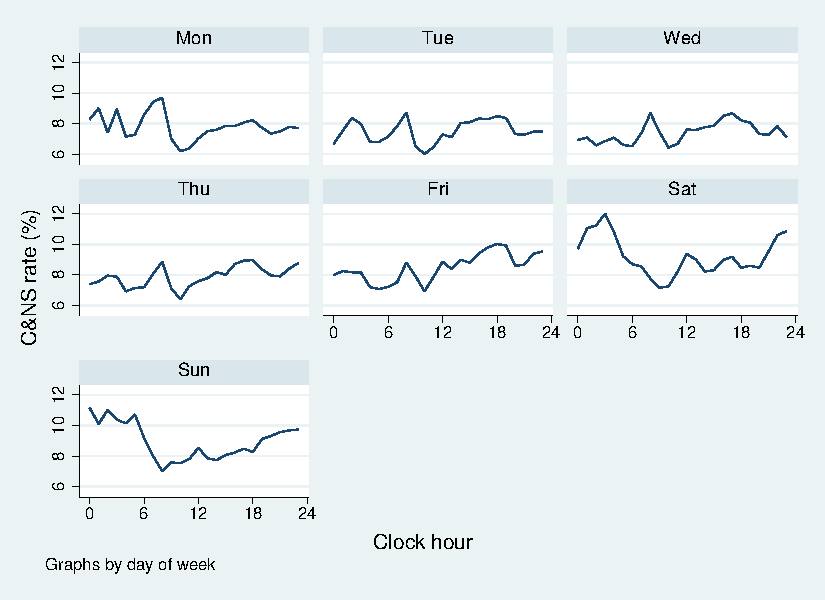
\includegraphics[width=0.8\linewidth]{./fg/cns_pct_dow.pdf}
% 	\caption{Percentage of cancellations and no-shows over total hourly bookings by day of week and hour of day}
% 	\label{fg:cancellations}
% \end{figure}

\begin{figure}
	{\centering
		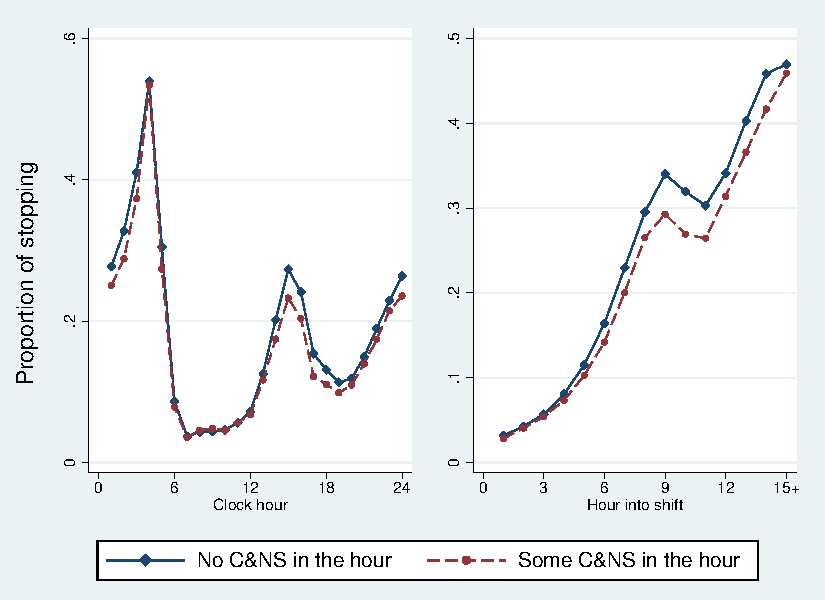
\includegraphics[width=0.75\textwidth]{./fg/modelfree_quit_vert.pdf}
		\caption{Proportion of drivers who stop work: with and without C\&NS}
		\label{fg:quitbyhour}
	}
%	{\justifying\footnotesize\emph{Notes:} The top panel shows the proportion of drivers who stop work after each hour of the day over the total number of drivers who work in that hour. The bottom panel shows the proportion of drivers who stop work after a certain number of hours into the shift over the total number of drivers who for at least that number of hours into the shift. The solid lines are for driver-hours in which there are no C\&NS. The dashed lines are for driver-hours in which there are some C\&NS.}
% \end{figure}

% \begin{figure}
	{\centering
		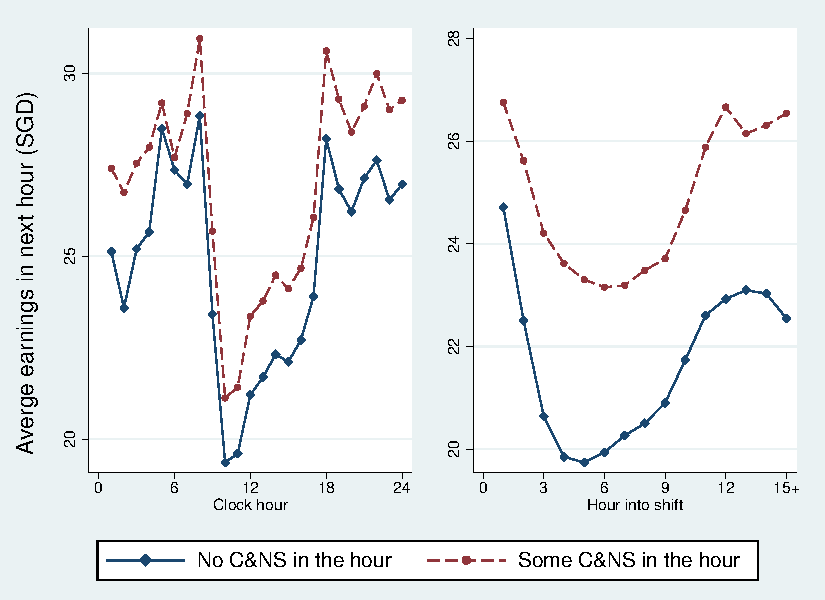
\includegraphics[width=0.75\textwidth]{./fg/modelfree_earnings_vert.pdf}
		\caption{Average hourly earnings in next: with and without C\&NS}
		\label{fg:earningsbyhour}
	}
%	{\justifying\footnotesize\emph{Notes:} The figure shows drivers' average earnings in the immediate hour following each hour of day (top panel) and hour into shift (bottom panel). The solid lines are for driver-hours in which there are no C\&NS. The dashed lines are for driver-hours in which there are some C\&NS.}
\end{figure}

\FloatBarrier

\begin{appendices}
	
\setcounter{figure}{0}
\renewcommand\thefigure{A\arabic{figure}}
\setcounter{table}{0}
\renewcommand\thetable{A\arabic{table}}

\FloatBarrier

\newpage

\section{Data cleaning}
\label{apx:DataCleaning}
The data cleaning process includes the following steps
\begin{itemize}[noitemsep,nolistsep]
	\item failed bookings (bookings for which the system failed to assign a taxi; 2.65\% of total observations)
	\item cancellations before confirmation (bookings that were cancelled before the system could assign a taxi; 2.00\%)
	\item observations with missing vehicle information (30 observations)
	\item observations with start date before December 1, 2016 or end time before start time (0.01\%)
	\item observations with trip duration shorter than 1 minutes or longer than 2 hours (0.25\%)
	\item observations with trip fare of value less than 3.2 SGD or more than 100 SGD (0.13\%)%\footnote{100 SGD is the 99.9725 percentile of the original trip fare distribution.}
	\item observations with trip distance shorter than 100 m or longer than 100 km (1.19\%)%\footnote{100 SGD is the 99.9725 percentile of the original trip fare distribution.}
	\item observations in a shift with shift duration less than 1 hour or more than 24 hours (1.82\%)
	\item observations in a shift with shift earnings less than 10 SGD or more than 1,000 SGD (0.01\%)%\footnote{1000 SGD is the 99.9725 percentile of the original shift income distribution.}
	\item duplicate trips/bookings, i.e., trips/bookings with the same start time and driver (0.3\%)
\end{itemize}

\section{Number of taxi trips and C\&NS rate by day of week and hour of day}
\FloatBarrier
\begin{figure}[!ht]
	\centering
	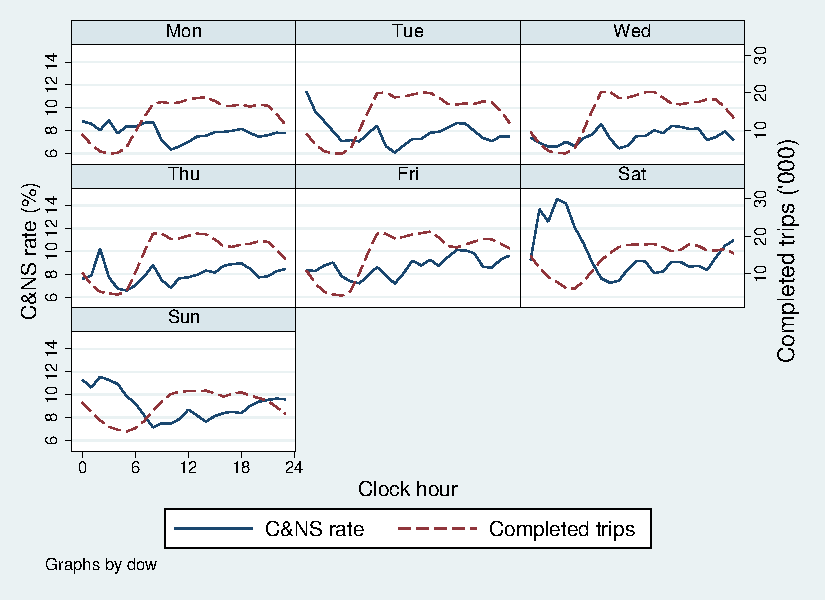
\includegraphics[width=0.8\textwidth]{./fg/dowplot.pdf}
	\caption{Average number of completed trips and rate of C\&NS by day of week and hour of day}
	\label{fg:trips}
\end{figure}


\FloatBarrier

\section{Proofs}
\label{apx:proofs}
\paragraph{Proof of Proposition~\ref{prop:unanticipated}} The net utility of continuing work
\[\Delta = V^{work} - V^{stop} = \begin{cases} 
(1+\lambda\eta)a_2 - c_2 + \epsilon_2 & \hbox{ if } u < t - a_1 - a_2 \\
(1+\eta)a_2 - (\lambda-1)\eta(a_1 + u - t) - c_2 + \epsilon_2 & \hbox{ if } t-a_1 \leq u < t - a_1 \\ 
(1+\eta)a_2 - c_2 + \epsilon_2 & \hbox{ if } u \geq t - a_1
\end{cases}\]
\[P(stop) = P(\Delta < 0) = P\left(\epsilon_2 < \begin{cases} 
c_2 - (1+\lambda\eta)a_2 & \hbox{ if } u < t - a_1 - a_2 \\
c_2 - (1+\eta)a_2 + (\lambda-1)\eta(a_1 + u - t) & \hbox{ if } t-a_1 \leq u < t - a_1 \\ 
c_2 - (1+\eta)a_2 & \hbox{ if } u \geq t - a_1\\
\end{cases}\right) 
\]
which is increasing in $u$. QED.

\paragraph{Proof of Proposition~\ref{prop:unanticipated}} Let $d^*(u) = 0$ if the driver stop when unanticipated earnings is $u$ and  $d^*(u) = 1$ when he/she continues.

The expected earnings under $d^*$ and parameter sets $(a_1, a_2, c_1, c_2)$ are 
\[t^* = E[a_1 + a_2d^*(u) + u]\]

The expected earnings under $d^*$ and parameter sets $(a_1+\delta, a_2, c_1, c_2)$ are
\[t' = E[a_1 + \delta + a_2d^*(u) + u] = \delta +E[a_1  + a_2d^*(u) + u] = t^* + \delta\]

Thus, $t^* + \delta$ is equal to the expected earnings under the decision $d^*$ and parameter set $(a_1+\delta, a_2, c_1, c_2)$.

Under the target $t^*$ and parameter set $(a_1, a_2, c_1, c_2)$, if the unanticipated earnings are $u$, net utility of working is 
\[\Delta(u|a_1, a_2, c_1, c_2, t^*) = a_2 - c_2 + l(a_1 + a_2 + u - t^*) -  l(a_1 + u - t^*) + \epsilon_2 \]


Under the target $t^*+\delta$ and parameter set $(a_1+\delta, a_2, c_1, c_2)$, if the unanticipated earnings are $u$, net utility of working is 
\[\Delta(u|a_1+\delta, a_2, c_1, c_2, t^*+\delta) = a_2  - c_2 + l(a_1 \delta + a_2 + u - (t^*+\delta)) -  l(a_1 + \delta + u - (t^*+\delta)) + \epsilon_2 \]

It is easy to see that \(\Delta(u|a_1, a_2, c_1, c_2, t^*)  = \Delta(u|a_1+\delta, a_2, c_1, c_2, t^*+\delta)\). Thus, if $d^*$ is optimal for \(\Delta(u|a_1, a_2, c_1, c_2, t^*) \), it must also be optimal for \(\Delta(u|a_1+\delta, a_2, c_1, c_2, t^*+\delta) \).


\paragraph{Proof of Proposition \ref{prop:effort}} The marginal cost of spending effort in the second period is 
\[MC = \frac{\partial c(e_1, e_2)}{\partial e_2} = c_2(e_1, e_2)\]
The marginal benefit of spending effort in the second period 
\[MB = \begin{cases}\eta &\hbox{ if } e_1+e_2+u > t\\\lambda\eta &\hbox{ if } e_1+e_2+u < t\end{cases}\]
Let $e_2^l$ and $e_2^h$ be the effort level such that $c_2(e_1, e_2^l) = \eta$ and $c_2(e_1, e_2^h) = \lambda\eta$. Since $c(e_1, e_2)$ is convex in $e_2$, $c_2(e_1, e_2)$ is increasing in $e_2$ and $e_2^h > e_2^l$.  The optimal level of effort in the second period is :
\[e_2^* = \begin{cases} e_1^l &\hbox{ if } t-e_1-u < e_2^l \\ t-e_1-u &\hbox{ if } e_2^l \leq t-e_1-u < e_2^h \\ e_2^h &\hbox{ if } t-e_1-u \geq e_2^h \end{cases}\]
which is decreasing in $u$


\paragraph{Proof of Proposition \ref{prop:ols1}}
OLS of $y$ on $i$ is
\[(i'i)^{-1}(i'y) = \frac{i'y/N}{i'i/N} \to \frac{Cov(i,y)}{V(i)} = \frac{Cov(u+a,\beta u + \epsilon)}{V(u+a)} = \beta\frac{V(u)}{V(u) + V(a)}\]

OLS of $y$ on $x$ is
\[(x'x)^{-1}(x'y) = \frac{x'y/N}{x'x/N} \to \frac{Cov(x,y)}{V(x)} = \frac{Cov(x,\beta (\gamma x + \omega) + \epsilon)}{V(x)} = \beta\gamma\]

OLS of $y$ on $x$ and $i$ is
\[\left(\begin{bmatrix}x\\i\end{bmatrix}'\begin{bmatrix}x\\i\end{bmatrix}\right)^{-1}\begin{bmatrix}x\\i\end{bmatrix}'y = \left(\begin{bmatrix}x'x & x'i \\ i'x & i'i\end{bmatrix}\right)^{-1}\begin{bmatrix} x'y\\i'y\end{bmatrix}=\frac{1}{(x'x)(i'i) - (x'i)^2)}\begin{bmatrix} (i'i)(x'y) - (x'i)(i'y)\\(x'x)(i'y)-(i'x)(x'y)\end{bmatrix}\] 

The first element converges to 
\[\frac{V(i)Cov(x,y) - Cov(x,i)Cov(i,y)}{V(x)V(i) - Cov(x,i)^2} = \beta\gamma\frac{V(a)}{V(a)+V(\omega)}\]

The second element converges to 
\[\frac{V(x)Cov(i,y) - Cov(x,i)Cov(x,y)}{V(x)V(i) - Cov(x,i)^2} = \beta\frac{V(\omega)}{V(a)+V(\omega)}\]

%\begin{center}
%	[Insert Table \ref{tb:robustmins} here]
%\end{center}

\newpage
\section{Effects of C\&NS on the remaining working time and the remaining idle percentage}
 	\begin{table}
 		\centering
 		\caption{Remaining work time (mins)}
 		\label{tb:robustmins}
            \setlength{\tabcolsep}{5pt}
 			\footnotesize
% 			{
\def\sym#1{\ifmmode^{#1}\else\(^{#1}\)\fi}
\begin{tabular}{l*{8}{S}}
\toprule
                    &\multicolumn{1}{c}{(1)}         &\multicolumn{1}{c}{(2)}         &\multicolumn{1}{c}{(3)}         &\multicolumn{1}{c}{(4)}         &\multicolumn{1}{c}{(5)}         &\multicolumn{1}{c}{(6)}         &\multicolumn{1}{c}{(7)}         &\multicolumn{1}{c}{(8)}         \\
\midrule
Cancellation (dummy)&      13.730\sym{***}&       4.825\sym{***}&       4.873\sym{***}&       5.597\sym{***}&       4.808\sym{***}&       5.560\sym{***}&       4.258\sym{***}&       4.792\sym{***}\\
                    &     (0.267)         &     (0.261)         &     (0.266)         &     (0.272)         &     (0.270)         &     (0.271)         &     (0.269)         &     (0.272)         \\
\addlinespace
No-show (dummy)     &      11.178\sym{***}&       4.863\sym{***}&       4.918\sym{***}&       5.711\sym{***}&       4.849\sym{***}&       5.585\sym{***}&       4.649\sym{***}&       6.419\sym{***}\\
                    &     (0.421)         &     (0.398)         &     (0.403)         &     (0.403)         &     (0.403)         &     (0.406)         &     (0.415)         &     (0.418)         \\
\addlinespace
Cumulative hours    &     -37.472\sym{***}&     -26.740\sym{***}&     -26.723\sym{***}&     -26.680\sym{***}&     -26.198\sym{***}&     -26.642\sym{***}&     -26.561\sym{***}&     -26.053\sym{***}\\
                    &     (0.162)         &     (0.203)         &     (0.203)         &     (0.203)         &     (0.203)         &     (0.203)         &     (0.206)         &     (0.206)         \\
\addlinespace
Cumulative income ('00 SGD)&     -34.899\sym{***}&     -42.529\sym{***}&     -42.546\sym{***}&     -42.436\sym{***}&     -52.237\sym{***}&     -42.432\sym{***}&     -42.428\sym{***}&     -52.298\sym{***}\\
                    &     (0.582)         &     (0.566)         &     (0.567)         &     (0.567)         &     (0.623)         &     (0.567)         &     (0.570)         &     (0.626)         \\
\addlinespace
Demand density      &       7.770\sym{***}&       4.549\sym{***}&      13.759\sym{***}&       8.262\sym{***}&       7.577\sym{***}&       8.306\sym{***}&       8.178\sym{***}&       7.780\sym{***}\\
                    &     (0.187)         &     (0.112)         &     (0.372)         &     (0.173)         &     (0.172)         &     (0.175)         &     (0.173)         &     (0.174)         \\
\addlinespace
Previous bookings (count)&                     &                     &                     &                     &       4.530\sym{***}&                     &                     &       4.625\sym{***}\\
                    &                     &                     &                     &                     &     (0.087)         &                     &                     &     (0.088)         \\
\addlinespace
Vehicles within 500m ('000)&                     &                     &                     &                     &                     &     -13.015\sym{***}&                     &      -4.893\sym{***}\\
                    &                     &                     &                     &                     &                     &     (1.219)         &                     &     (1.222)         \\
\addlinespace
Distance to pickup (km)&                     &                     &                     &                     &                     &                     &       0.143         &      -0.661\sym{***}\\
                    &                     &                     &                     &                     &                     &                     &     (0.173)         &     (0.177)         \\
\addlinespace
On-call duration (mins)&                     &                     &                     &                     &                     &                     &       0.304\sym{***}&      -0.335\sym{***}\\
                    &                     &                     &                     &                     &                     &                     &     (0.030)         &     (0.031)         \\
\addlinespace
Driver FE           &       {Yes}         &       {Yes}         &       {Yes}         &       {Yes}         &       {Yes}         &       {Yes}         &       {Yes}         &       {Yes}         \\
\addlinespace
Date FE           &       {-}         &       {Yes}         &       {Yes}         &       {Yes}         &       {Yes}         &       {Yes}         &       {Yes}         &       {Yes}         \\
\addlinespace
Hour\(\times\)day of week FE&         {-}         &       {Yes}         &       {Yes}         &         {-}         &         {-}         &         {-}         &         {-}         &         {-}         \\
\addlinespace
Postal code FE      &         {-}         &         {-}         &       {Yes}         &         {-}         &         {-}         &         {-}         &         {-}         &         {-}         \\
\addlinespace
Hour\(\times\)day of week\(\times\)Zone FE&         {-}         &         {-}         &         {-}         &       {Yes}         &       {Yes}         &       {Yes}         &       {Yes}         &       {Yes}         \\
\midrule
Observations        &\num{31563560}         &\num{31563560}         &\num{28528407}         &\num{28510154}         &\num{28510154}         &\num{28192061}         &\num{28118335}         &\num{27805742}         \\
$R^2$             &     {0.596}         &     {0.634}         &     {0.636}         &     {0.636}         &     {0.636}         &     {0.635}         &     {0.637}         &     {0.637}         \\
\bottomrule
\end{tabular}
}

            {
            \def\sym#1{\ifmmode^{#1}\else\(^{#1}\)\fi}
            \begin{tabular}{l*{8}{S}}
            \toprule
            \toprule
                                &\multicolumn{1}{c}{(1)}         &\multicolumn{1}{c}{(2)}         &\multicolumn{1}{c}{(3)}         &\multicolumn{1}{c}{(4)}         &\multicolumn{1}{c}{(5)}         &\multicolumn{1}{c}{(6)}         &\multicolumn{1}{c}{(7)}         &\multicolumn{1}{c}{(8)}         \\
            \midrule
            Cancellation (dummy)&      11.66&       4.04&       4.40&       4.70&       4.21&       4.61&       3.62&       4.24\\
                                &     (0.26)         &     (0.26)         &     (0.26)         &     (0.27)         &     (0.27)         &     (0.27)         &     (0.27)         &     (0.27)         \\
            \addlinespace
            No-show (dummy)     &       9.17&       3.93&       4.26&       4.70&       4.18&       4.63&       4.13&       5.93\\
                                &     (0.42)         &     (0.39)         &     (0.40)         &     (0.40)         &     (0.40)         &     (0.40)         &     (0.41)         &     (0.42)         \\
            \addlinespace
            Cumulative hours    &     -36.96&     -26.33&     -26.33&     -26.28&     -25.91&     -26.24&     -26.16&     -25.77\\
                                &     (0.17)         &     (0.20)         &     (0.20)         &     (0.20)         &     (0.20)         &     (0.20)         &     (0.21)         &     (0.21)         \\
            \addlinespace
            Cumulative income ('00 SGD)&     -37.79&     -44.88&     -44.78&     -44.70&     -53.54&     -44.68&     -44.66&     -53.61\\
                                &     (0.60)         &     (0.58)         &     (0.58)         &     (0.58)         &     (0.63)         &     (0.58)         &     (0.58)         &     (0.63)         \\
            \addlinespace
            Demand density      &       4.59&       3.12&       6.12&       3.60&       3.11&       3.65&       3.63&       3.34\\
                                &     (0.18)         &     (0.11)         &     (0.35)         &     (0.16)         &     (0.16)         &     (0.16)         &     (0.16)         &     (0.16)         \\
            \addlinespace
            Previous bookings (count)&                     &                     &                     &                     &       4.29&                     &                     &       4.39\\
                                &                     &                     &                     &                     &     (0.09)         &                     &                     &     (0.09)         \\
            \addlinespace
            Vehicles within 500m ('000)&                     &                     &                     &                     &                     &      -8.89&                     &      -4.40\\
                                &                     &                     &                     &                     &                     &     (1.18)         &                     &     (1.19)         \\
            \addlinespace
            Distance to pickup (km)&                     &                     &                     &                     &                     &                     &      -0.14         &      -0.80\\
                                &                     &                     &                     &                     &                     &                     &     (0.17)         &     (0.18)         \\
            \addlinespace
            Oncall duration (mins)&                     &                     &                     &                     &                     &                     &       0.21&      -0.37\\
                                &                     &                     &                     &                     &                     &                     &     (0.03)         &     (0.03)         \\
            \addlinespace
            Driver FE           &       {Yes}         &       {Yes}         &       {Yes}         &       {Yes}         &       {Yes}         &       {Yes}         &       {Yes}         &       {Yes}         \\
            \addlinespace
            Hour\(\times\)day of week FE&         {-}         &       {Yes}         &       {Yes}         &         {-}         &         {-}         &         {-}         &         {-}         &         {-}         \\
            \addlinespace
            Postal code FE      &         {-}         &         {-}         &       {Yes}         &         {-}         &         {-}         &         {-}         &         {-}         &         {-}         \\
            \addlinespace
            Hour\(\times\)day of week\(\times\)Zone FE&         {-}         &         {-}         &         {-}         &       {Yes}         &       {Yes}         &       {Yes}         &       {Yes}         &       {Yes}         \\
            \addlinespace
            date                &       {Yes}         &       {Yes}         &       {Yes}         &       {Yes}         &       {Yes}         &       {Yes}         &       {Yes}         &       {Yes}         \\
            \midrule
            Observations        &\num{31108572}         &\num{31108572}         &\num{28087962}         &\num{28069984}         &\num{28069984}         &\num{27757937}         &\num{27683044}         &\num{27375698}         \\
            \(R^2\)             &     {0.601}         &     {0.636}         &     {0.638}         &     {0.638}         &     {0.638}         &     {0.637}         &     {0.639}         &     {0.639}         \\
            \bottomrule
            \end{tabular}
            }
 			\begin{tablenotes}
 				Each column is a separate regression. An observation is a trip or a booking. The dependent variable for all columns is the remaining work time in  minutes, i.e., the number of minutes from the end of the trip/booking to the end of the respective shift. Standard errors clustered by drivers in parentheses. 
 			\end{tablenotes}
 	\end{table}



%\begin{center}
%	[Insert Table \ref{tb:robustidle} here]
%\end{center}
\FloatBarrier

%\begin{landscape}
	\begin{table}[h]
 		\centering
 		\caption{Idle percentage after a trip/booking (\%)}
 		\label{tb:robustidle}
		
 		% \begin{threeparttable}
 			\footnotesize
 			\setlength{\tabcolsep}{2pt}
 			% {
\def\sym#1{\ifmmode^{#1}\else\(^{#1}\)\fi}
\begin{tabular}{l*{8}{S}}
\toprule
                    &\multicolumn{1}{c}{(1)}         &\multicolumn{1}{c}{(2)}         &\multicolumn{1}{c}{(3)}         &\multicolumn{1}{c}{(4)}         &\multicolumn{1}{c}{(5)}         &\multicolumn{1}{c}{(6)}         &\multicolumn{1}{c}{(7)}         &\multicolumn{1}{c}{(8)}         \\
\midrule
Cancellation (dummy)&      -1.515\sym{***}&      -1.161\sym{***}&      -1.218\sym{***}&      -0.894\sym{***}&      -0.897\sym{***}&      -0.746\sym{***}&      -0.772\sym{***}&      -0.724\sym{***}\\
                    &     (0.023)         &     (0.022)         &     (0.022)         &     (0.022)         &     (0.022)         &     (0.022)         &     (0.023)         &     (0.023)         \\
\addlinespace
No-show (dummy)     &      -0.704\sym{***}&      -0.225\sym{***}&      -0.313\sym{***}&       0.052         &       0.049         &       0.200\sym{***}&       0.312\sym{***}&       0.334\sym{***}\\
                    &     (0.036)         &     (0.035)         &     (0.035)         &     (0.035)         &     (0.035)         &     (0.035)         &     (0.036)         &     (0.036)         \\
\addlinespace
Cumulative hours    &      -1.616\sym{***}&      -1.209\sym{***}&      -1.185\sym{***}&      -1.177\sym{***}&      -1.176\sym{***}&      -1.182\sym{***}&      -1.156\sym{***}&      -1.158\sym{***}\\
                    &     (0.012)         &     (0.011)         &     (0.011)         &     (0.011)         &     (0.011)         &     (0.011)         &     (0.011)         &     (0.011)         \\
\addlinespace
Cumulative income ('00 SGD)&       5.812\sym{***}&       4.329\sym{***}&       4.234\sym{***}&       4.208\sym{***}&       4.168\sym{***}&       4.215\sym{***}&       4.091\sym{***}&       4.054\sym{***}\\
                    &     (0.049)         &     (0.046)         &     (0.046)         &     (0.046)         &     (0.046)         &     (0.046)         &     (0.045)         &     (0.045)         \\
\addlinespace
Demand density      &      -2.315\sym{***}&      -1.677\sym{***}&      -3.760\sym{***}&      -1.537\sym{***}&      -1.540\sym{***}&      -1.569\sym{***}&      -1.545\sym{***}&      -1.591\sym{***}\\
                    &     (0.016)         &     (0.012)         &     (0.029)         &     (0.018)         &     (0.018)         &     (0.019)         &     (0.018)         &     (0.019)         \\
\addlinespace
Previous bookings (count)&                     &                     &                     &                     &       0.018\sym{**} &                     &                     &       0.018\sym{**} \\
                    &                     &                     &                     &                     &     (0.008)         &                     &                     &     (0.008)         \\
\addlinespace
Vehicles within 500m ('000)&                     &                     &                     &                     &                     &       9.606\sym{***}&                     &       9.337\sym{***}\\
                    &                     &                     &                     &                     &                     &     (0.098)         &                     &     (0.099)         \\
\addlinespace
Distance to pickup (km)&                     &                     &                     &                     &                     &                     &      -0.328\sym{***}&      -0.225\sym{***}\\
                    &                     &                     &                     &                     &                     &                     &     (0.015)         &     (0.014)         \\
\addlinespace
On-call duration (mins)&                     &                     &                     &                     &                     &                     &      -0.051\sym{***}&      -0.030\sym{***}\\
                    &                     &                     &                     &                     &                     &                     &     (0.003)         &     (0.003)         \\
\addlinespace
Driver FE           &       {Yes}         &       {Yes}         &       {Yes}         &       {Yes}         &       {Yes}         &       {Yes}         &       {Yes}         &       {Yes}         \\
\addlinespace
Date FE           &       {-}         &       {Yes}         &       {Yes}         &       {Yes}         &       {Yes}         &       {Yes}         &       {Yes}         &       {Yes}         \\
\addlinespace
Hour\(\times\)day of week FE&         {-}         &       {Yes}         &       {Yes}         &         {-}         &         {-}         &         {-}         &         {-}         &         {-}         \\
\addlinespace
Postal code FE      &         {-}         &         {-}         &       {Yes}         &         {-}         &         {-}         &         {-}         &         {-}         &         {-}         \\
\addlinespace
Hour\(\times\)day of week\(\times\)Zone FE&         {-}         &         {-}         &         {-}         &       {Yes}         &       {Yes}         &       {Yes}         &       {Yes}         &       {Yes}         \\
\midrule
Observations        &\num{26511775}         &\num{26511775}         &\num{23821515}         &\num{23808266}         &\num{23808266}         &\num{23543680}         &\num{23469766}         &\num{23209593}         \\
$R^2$             &     {0.320}         &     {0.365}         &     {0.372}         &     {0.373}         &     {0.373}         &     {0.373}         &     {0.374}         &     {0.374}         \\
\bottomrule
\end{tabular}
}

				{
				\def\sym#1{\ifmmode^{#1}\else\(^{#1}\)\fi}
				\begin{tabular}{l*{8}{S}}
				\toprule
				\toprule
				                    &\multicolumn{1}{c}{(1)}         &\multicolumn{1}{c}{(2)}         &\multicolumn{1}{c}{(3)}         &\multicolumn{1}{c}{(4)}         &\multicolumn{1}{c}{(5)}         &\multicolumn{1}{c}{(6)}         &\multicolumn{1}{c}{(7)}         &\multicolumn{1}{c}{(8)}         \\
				\midrule
				Cancellation (dummy)&      -1.515&      -1.161&      -1.218&      -0.894&      -0.897&      -0.746&      -0.772&      -0.724\\
				                    &     (0.023)         &     (0.022)         &     (0.022)         &     (0.022)         &     (0.022)         &     (0.022)         &     (0.023)         &     (0.023)         \\
				\addlinespace
				No-show (dummy)     &      -0.704&      -0.225&      -0.313&       0.052         &       0.049         &       0.200&       0.312&       0.334\\
				                    &     (0.036)         &     (0.035)         &     (0.035)         &     (0.035)         &     (0.035)         &     (0.035)         &     (0.036)         &     (0.036)         \\
				\addlinespace
				Cumulative hours    &      -1.616&      -1.209&      -1.185&      -1.177&      -1.176&      -1.182&      -1.156&      -1.158\\
				                    &     (0.012)         &     (0.011)         &     (0.011)         &     (0.011)         &     (0.011)         &     (0.011)         &     (0.011)         &     (0.011)         \\
				\addlinespace
				Cumulative income ('00 SGD)&       5.812&       4.329&       4.234&       4.208&       4.168&       4.215&       4.091&       4.054\\
				                    &     (0.049)         &     (0.046)         &     (0.046)         &     (0.046)         &     (0.046)         &     (0.046)         &     (0.045)         &     (0.045)         \\
				\addlinespace
				Demand density      &      -2.315&      -1.677&      -3.760&      -1.537&      -1.540&      -1.569&      -1.545&      -1.591\\
				                    &     (0.016)         &     (0.012)         &     (0.029)         &     (0.018)         &     (0.018)         &     (0.019)         &     (0.018)         &     (0.019)         \\
				\addlinespace
				Previous bookings (count)&                     &                     &                     &                     &       0.018 &                     &                     &       0.018 \\
				                    &                     &                     &                     &                     &     (0.008)         &                     &                     &     (0.008)         \\
				\addlinespace
				Vehicles within 500m ('000)&                     &                     &                     &                     &                     &       9.606&                     &       9.337\\
				                    &                     &                     &                     &                     &                     &     (0.098)         &                     &     (0.099)         \\
				\addlinespace
				Distance to pickup (km)&                     &                     &                     &                     &                     &                     &      -0.328&      -0.225\\
				                    &                     &                     &                     &                     &                     &                     &     (0.015)         &     (0.014)         \\
				\addlinespace
				On-call duration (mins)&                     &                     &                     &                     &                     &                     &      -0.051&      -0.030\\
				                    &                     &                     &                     &                     &                     &                     &     (0.003)         &     (0.003)         \\
				\addlinespace
				Driver FE           &       {Yes}         &       {Yes}         &       {Yes}         &       {Yes}         &       {Yes}         &       {Yes}         &       {Yes}         &       {Yes}         \\
				\addlinespace
				Date FE           &       {-}         &       {Yes}         &       {Yes}         &       {Yes}         &       {Yes}         &       {Yes}         &       {Yes}         &       {Yes}         \\
				\addlinespace
				Hour\(\times\)day of week FE&         {-}         &       {Yes}         &       {Yes}         &         {-}         &         {-}         &         {-}         &         {-}         &         {-}         \\
				\addlinespace
				Postal code FE      &         {-}         &         {-}         &       {Yes}         &         {-}         &         {-}         &         {-}         &         {-}         &         {-}         \\
				\addlinespace
				Hour\(\times\)day of week\(\times\)Zone FE&         {-}         &         {-}         &         {-}         &       {Yes}         &       {Yes}         &       {Yes}         &       {Yes}         &       {Yes}         \\
				%\midrule
				\addlinespace
				Observations        &\num{26511775}         &\num{26511775}         &\num{23821515}         &\num{23808266}         &\num{23808266}         &\num{23543680}         &\num{23469766}         &\num{23209593}         \\
				$R^2$             &     {0.320}         &     {0.365}         &     {0.372}         &     {0.373}         &     {0.373}         &     {0.373}         &     {0.374}         &     {0.374}         \\
				\bottomrule
				\end{tabular}
				}
 			\begin{tablenotes}
 				Each column is a separate regression. An observation is a trip or a booking. The dependent variable for all columns is the remaining idle percentage, i.e., percentage of time a driver is with a passenger during the remaining time (i.e., from the end of the trip/booking to the end of the shift). Standard errors clustered by drivers in parentheses. 
 			\end{tablenotes}
 		% \end{threeparttable}
 	\end{table}
% \end{landscape}
\FloatBarrier

\section{Instrumental-variable regression}
\label{apx:iv}
Due to the fact that customers pay no penalties for C\&NS, one of the common reasons for C\&NS 
is passengers hailing a random taxicab that just happens to pass by while waiting for the booked driver to arrive. 
Since the drivers do not coordinate with each other, the chance of a passenger seeing a random
free taxicab can be considered as exogenous to the the booked driver' labor decisions.
As a result, we can use the number of nearby free taxi vehicles around the time of 
booking as a valid instrumental variable for the occurrence of C\&NS.
Specifically, we will use the number of free taxi vehicles within 3 minutes after booking, 
within 100-m radius and within 200-m radius from the pickup location as the instrumental
variables. We control for postal code by hour-of-day by day-of-week fixed effects as
well as the number of vehicles within 500 m and 1 km to absorb the spatiotemporal distribution
taxi supply over the city. Thus, the variation of C\&NS that we use here is the change in C\&NS
due to free taxicabs moving around locally, keeping the broader market supply at 500 m and 1 km 
radius constant. 

Table \ref{tb:iv} reports the results. Since the difference in magnitude of the cancellation effect
and the no-show effect on the hazard rate of stopping is small, 
and to increase the power of the IV estimates, we create
a common dummy variable for C\&NS. We also limit our sample to bookings, because the construction
of free vehicle count at booking time is not well defined for street hail trips.
Column (1) reports the OLS estimates using this new
independent variable, and the estimated effect, at $-0.199$ (s.e. $0.0003$) is similar 
to previous results.
Column (2) and (3) report the first-stage and second-stage estimates of the IV regression.
Column (2) shows that the number of free vehicles within 100-m and 200-m radius from 
the pickup location increases the chance of C\&NS, consistent with the story that
passengers cancel and fail to show up because of random free taxicab passing by.
The estimates are significant at 1\% level, indicating strong relationship between
the instrumental variables and the independent variable.
Column (3) shows that C\&NS  which are due to free taxicabs nearby the pickup location
tend to decreases the hazard of stopping work for the booked driver by 3.8 ppts (s.e. 1.8).
The IV estimate is larger in magnitude than the OLS estimate, but less precise.
The exogeneity test, with p-value of 0.24, fails to reject the hypothesis that
the independent variables is exogenous.
The F-statistics of weak-identification test is 888, strongly rejecting the hypothesis
the the instrumental variables are weak.


\FloatBarrier
\begin{table}
    \centering
    \footnotesize
    \caption{Hazard rate of stopping work: IV regression}
    \label{tb:iv}
{
\def\sym#1{\ifmmode^{#1}\else\(^{#1}\)\fi}
\begin{tabularx}{\textwidth}{l@{\extracolsep{\fill}}*{3}{S}} 
%\begin{tabular}{l*{3}{c}}
\toprule
\toprule
            &\multicolumn{1}{c}{OLS} &\multicolumn{2}{c}{2SLS}\\
            \cmidrule(lr){2-2} \cmidrule(lr){3-4}
            &\multicolumn{1}{c}{(1)}&\multicolumn{1}{c}{(2)}&\multicolumn{1}{c}{(3)}\\
\textit{Dependent variable} &\multicolumn{1}{c}{Quit}&\multicolumn{1}{c}{C\&NS}&\multicolumn{1}{c}{Quit}\\
\midrule
C\&NS (dummy)&     -0.0199\sym{***}&                     &     -0.0389\sym{**} \\
            &    (0.0003)         &                     &    (0.0176)         \\
\addlinespace
Free vehicle within 100 m (count)&                     &      0.0028\sym{***}&                     \\
            &                     &    (0.0001)         &                     \\
\addlinespace
Free vehicle within 200 m (count)&                     &      0.0004\sym{***}&                     \\
            &                     &    (0.0001)         &                     \\
\midrule
Observations&\num{6103669}         &\num{6103669}         &\num{6103669}         \\
\(R^2\)     &       0.283         &       0.277         &       0.050         \\
Weak-identification F-statistic&                     &                     &         888         \\
Exogeneity test \(\chi^2\)-statistic&                     &                     &       1.377         \\
            &                     &                     &     [0.241]         \\
\bottomrule
\end{tabularx}
}

 			\begin{tablenotes}
 			 An observation is a booking. All regressions include driver fixed effects, date fixed effects, hour$\times$day-of-week$\times$postal-code fixed effects, demand, free vehicle count within 500 m and 1 km radius from pickup location, and a cubic function of cumulative hours. Standard errors clustered by drivers in parentheses. p-value of tests in bracket.
 			\end{tablenotes}

\end{table}

\end{appendices}


\end{document}

